\chapter{分治}
\label{ch:dc}

% 本章的圖共用的樣式（名稱都以 dc 開頭，避免和其他章衝突）
\tikzset{
    dc-cell/.style={draw=black!55, minimum width=0.8cm, minimum height=0.62cm, inner sep=0pt, font=\small},
    dc-run/.style={dc-cell, fill=coreFill, draw=coreStroke},
    dc-ghost/.style={dc-cell, draw=black!30, dashed, text=black!45},
    dc-arr/.style={-{Stealth[length=1.8mm]}, draw=black!65},
    dc-tn/.style={draw=black!55, rounded corners=2pt, inner sep=2.5pt, font=\scriptsize, align=center, fill=white},
    dc-tnw/.style={dc-tn, draw=memStroke, thick, fill=memFill},
    dc-leaf/.style={draw=black!40, rounded corners=2pt, inner sep=2pt, font=\scriptsize, minimum width=0.75cm, align=center},
    dc-edge/.style={draw=black!55},
    dc-pt/.style={circle, fill=black!80, inner sep=0pt, minimum size=4.2pt},
    dc-ptlab/.style={font=\scriptsize, inner sep=1.5pt},
    dc-ray/.style={draw=black!35, dashed},
    dc-rayq/.style={-{Stealth[length=1.8mm]}, dashed, draw=optStroke},
    dc-vec/.style={-{Stealth[length=2mm]}, thick, draw=black!75},
    dc-seg/.style={thick, draw=black!80},
    dc-seg2/.style={thick, draw=coreStroke},
}

夜市一個飲料攤把開張以來每天的盈虧記在本子上，賺錢記正數，賠錢記負數。 老闆想找
出「連續幾天加起來賺最多」的那一段，回頭看那幾天做對了什麼。 一年有三百多天，每
一段都加加看，要試五萬多段。 如果先把這一年從中間切成上半年和下半年，賺最多的那
一段只可能落在哪幾種地方？ 每一種地方各要花多少工夫才找得到？ 往下讀之前，先想
一想。

第~14~章的合併排序把陣列切成兩半，兩半各自排好，再合併起來。 這種做法叫
\textbf{分治法}（divide and conquer），每一層遞迴都做三件事：

\begin{enumerate}
\item \textbf{分}（divide）：把問題切成幾個同類型、規模比較小的子問題。
\item \textbf{治}（conquer）：用同樣的方法遞迴解每個子問題；規模夠小時直接解。
\item \textbf{合}（combine）：把子問題的答案組合成原問題的答案。
\end{enumerate}

切成 $a$ 個規模 $n/b$ 的子問題、分和合一共花 $f(n)$ 時，執行時間是
$T(n) = aT(n/b) + f(n)$，用第~2~章的遞迴樹或主定理（定理~\ref{thm:rec-master}）就能解。 這個式子
也告訴我們，想讓分治法變快，有兩個方向：讓 $f(n)$ 變小（合得更省），或讓 $a$ 變
小（少解幾個子問題）。 這一章的前五節分別示範幾種情形，第六節是計算幾何入門。

\begin{itemize}
\item 第~\ref{sec:dc-bsearch}~節的二分搜尋和快速冪只需要解\textbf{一個}子問題，
$a = 1$。
\item 第~\ref{sec:dc-maxsub}~節的最大子陣列，難的是「合」：最好的一段可能跨過切
開的地方。 這一節最後會用一個線性時間的做法和分治版對照。
\item 第~\ref{sec:dc-mult}~節的 Karatsuba 大數乘法和 Strassen 矩陣乘法，靠代數把
子問題的個數從 $4$ 減成 $3$、從 $8$ 減成 $7$，指數就跟著變小。
\item 第~\ref{sec:dc-closest}~節的平面最近點對，「合」的步驟要靠一個幾何的論證，
才能在線性時間內完成。
\item 第~\ref{sec:dc-inv}~節的逆序數計數，把計數藏在合併排序的合併步驟裡。
\item 第~\ref{sec:dc-geom}~節是計算幾何入門：用外積判斷轉向、線段相交、點在多邊形內，
以及凸包。 凸包的分治做法和最近點對同一個結構；它的 $\Omega(n \lg n)$ 下界則是把排序
歸約到凸包得到的。
\end{itemize}

子問題如果彼此重疊，同一個子問題會被解很多次，分治法就不划算了，這時要改用第~18~
章的動態規劃。

這一章用到第~1~章的迴圈不變量和逆序對、第~2~章的遞迴式和主定理、第~14~章的合併；
最後一節還用到第~3~章的聚合法、第~6~章的堆疊和第~15~章的排序下界。
C 程式用到《C 程式設計基礎》第~9~章的指標參數、第~14~章的結構、第~15~章的遞迴、第~18~章
的 \texttt{qsort} 和第~19~章的 \texttt{malloc}；遞迴在第~2~章複習過，其他的用到時先在框
裡複習。

\section{二分搜尋與快速冪}
\label{sec:dc-bsearch}

分治不一定要把每一份都解。 如果比一次就能判斷答案只可能在哪一份，另一份就整個丟
掉，遞迴式變成 $T(n) = T(n/b) + f(n)$。 有些書把這種只留一個子問題的情形叫做「減
而治之」（decrease and conquer）。 這一節的兩個例子都屬於這一類。

\subsection{找一個值}

輸入是由小到大排好（允許相等）的 $A[1..n]$ 和一個數 $x$。 如果 $x$ 在裡面，回傳
一個位置 $i$ 使 $A[i] = x$；不在就回傳 \NIL。 第~2~章的虛擬碼~\ref{alg:rec-search} 是遞迴版：看中
間那一格，相等就回答，比 $x$ 小就到右半邊找，比 $x$ 大就到左半邊找。 遞迴呼叫是
函式的最後一步（第~6~章的尾遞迴），所以可以直接改成迴圈，用 $\mathit{lo}$、
$\mathit{hi}$ 記住還要找的範圍 $A[\mathit{lo}..\mathit{hi}]$。

\begin{pseudo}[label=alg:dc-bsearch]{二分搜尋（閉區間）}
\Function{Binary-Search}{$A, n, x$}
    \State $\mathit{lo} \gets 1$；$\mathit{hi} \gets n$
    \While{$\mathit{lo} \le \mathit{hi}$}
        \State $\mathit{mid} \gets \lfloor (\mathit{lo} + \mathit{hi}) / 2 \rfloor$
        \If{$A[\mathit{mid}] = x$}
            \State \Return $\mathit{mid}$
        \ElsIf{$A[\mathit{mid}] < x$}
            \State $\mathit{lo} \gets \mathit{mid} + 1$
        \Else
            \State $\mathit{hi} \gets \mathit{mid} - 1$
        \EndIf
    \EndWhile
    \State \Return \NIL
\EndFunction
\end{pseudo}

\textbf{不變量}：每次檢查第 3 行的條件時，$A[1..\mathit{lo}-1]$ 的每個數都小於
$x$，$A[\mathit{hi}+1..n]$ 的每個數都大於 $x$。 照第~\ref{sec:ana-invariant}~節的三步來證。

\begin{itemize}
\item \textbf{初始}：$\mathit{lo} = 1$、$\mathit{hi} = n$，兩段都是空的，敘述成立。
\item \textbf{維持}：迴圈裡 $\mathit{lo} \le \mathit{mid} \le \mathit{hi}$，所以
$A[\mathit{mid}]$ 存在。 如果 $A[\mathit{mid}] = x$，程序直接回傳，不必維持。 如
果 $A[\mathit{mid}] < x$，因為陣列排好了，$A[\mathit{lo}..\mathit{mid}]$ 都不大於
$A[\mathit{mid}]$，也就都小於 $x$；第 8 行把 $\mathit{lo}$ 改成 $\mathit{mid} +
1$ 之後，$A[1..\mathit{lo}-1]$ 仍然都小於 $x$。 $A[\mathit{mid}] > x$ 的情形對稱，
$A[\mathit{mid}..\mathit{hi}]$ 都大於 $x$，第 10 行之後第二段仍然成立。
\item \textbf{結束}：如果是第 6 行回傳，$A[\mathit{mid}] = x$，答案正確。 否則迴
圈停在 $\mathit{lo} = \mathit{hi} + 1$（每一輪 $\mathit{lo}$ 最多跳到
$\mathit{hi} + 1$，$\mathit{hi}$ 最少降到 $\mathit{lo} - 1$），代進不變量：
$A[1..\mathit{hi}]$ 都小於 $x$，$A[\mathit{hi}+1..n]$ 都大於 $x$，整個陣列沒有一
個等於 $x$，回傳 \NIL{} 正確。
\end{itemize}

\textbf{一定會停，而且很快}。 令 $k = \mathit{hi} - \mathit{lo} + 1$ 是還要找的
格數。 中間那格左邊剩 $\mathit{mid} - \mathit{lo} = \lfloor (k-1)/2 \rfloor$ 格，
右邊剩 $\mathit{hi} - \mathit{mid} = \lceil (k-1)/2 \rceil = \lfloor k/2 \rfloor$
格，所以每一輪之後 $k$ 最多剩 $\lfloor k/2 \rfloor$。 $t$ 輪之後
$k \le \lfloor n / 2^t \rfloor$；$t = \lfloor \lg n \rfloor + 1$ 時 $n / 2^t < 1$，
範圍已經是空的。 所以迴圈最多跑 $\lfloor \lg n \rfloor + 1$ 輪，每一輪 $\Theta(1)$，
最壞情況 $\Theta(\lg n)$。 這和第~2~章算出的遞迴版一致。

\subsection{第一個大於等於、第一個大於}

用 $A = \langle 12, 15, 15, 15, 23, 31, 31, 40 \rangle$ 找 $x = 15$：第一輪
$\mathit{mid} = 4$，$A[4] = 15$，馬上回傳 $4$。 $15$ 出現在第 $2$、$3$、$4$ 格，
\proc{Binary-Search} 回傳的是\textbf{其中一個}，不一定是第一個。 很多問題要的是
邊界：第一個 $15$ 在哪裡、$15$ 有幾個、比 $20$ 小的最後一個數在哪裡。 這時改用兩
個「找邊界」的版本：

\begin{itemize}
\item \proc{Lower-Bound}$(A, n, x)$：第一個滿足 $A[i] \ge x$ 的位置 $i$；全部都小
於 $x$ 時回傳 $n + 1$。
\item \proc{Upper-Bound}$(A, n, x)$：第一個滿足 $A[i] > x$ 的位置 $i$；全部都不大
於 $x$ 時回傳 $n + 1$。
\end{itemize}

\proc{Lower-Bound} 的虛擬碼和正確性證明在第~1~章觀念題第~\ref{ana-q-lower-bound}~題。 它用的是
\textbf{半開區間}：答案一定在 $\mathit{lo}..\mathit{hi}$ 之間（可能等於
$\mathit{hi}$），$\mathit{hi}$ 從 $n + 1$ 開始，迴圈條件是 $\mathit{lo} <
\mathit{hi}$，往左縮時寫 $\mathit{hi} \gets \mathit{mid}$。 \proc{Upper-Bound} 只
差一個比較符號：

\begin{pseudo}[label=alg:dc-upper]{第一個大於 $x$ 的位置（半開區間）}
\Function{Upper-Bound}{$A, n, x$}
    \State $\mathit{lo} \gets 1$；$\mathit{hi} \gets n + 1$
    \While{$\mathit{lo} < \mathit{hi}$}
        \State $\mathit{mid} \gets \lfloor (\mathit{lo} + \mathit{hi}) / 2 \rfloor$
        \If{$A[\mathit{mid}] \le x$}
            \State $\mathit{lo} \gets \mathit{mid} + 1$
        \Else
            \State $\mathit{hi} \gets \mathit{mid}$
        \EndIf
    \EndWhile
    \State \Return $\mathit{lo}$
\EndFunction
\end{pseudo}

不變量換成：$A[1..\mathit{lo}-1]$ 都不大於 $x$，$A[\mathit{hi}..n]$ 都大於 $x$。
證明和第~1~章那一題逐字相同，只要把「小於 $x$」換成「不大於 $x$」、「大於等於
$x$」換成「大於 $x$」。 每一輪 $\mathit{hi} - \mathit{lo}$ 從 $k$ 變成
$\lfloor k/2 \rfloor$ 或 $\lceil k/2 \rceil - 1$，都不超過 $\lfloor k/2 \rfloor$，
所以迴圈最多跑 $\lfloor \lg n \rfloor + 1$ 輪。 兩個版本在找不到時都不必另外處
理，這是半開區間寫法的好處。

用上面的陣列手算。 每一列是一輪迴圈開始時的 $\mathit{lo}$、$\mathit{hi}$，以及這
一輪的 $\mathit{mid}$ 和改了哪一邊。

\begin{center}
\begin{tabular}{cccccl}
\toprule
& $\mathit{lo}$ & $\mathit{hi}$ & $\mathit{mid}$ & $A[\mathit{mid}]$ & 動作 \\
\midrule
\proc{Lower-Bound}$(A, 8, 15)$ & 1 & 9 & 5 & 23 & $23 \ge 15$，$\mathit{hi} \gets 5$ \\
& 1 & 5 & 3 & 15 & $15 \ge 15$，$\mathit{hi} \gets 3$ \\
& 1 & 3 & 2 & 15 & $15 \ge 15$，$\mathit{hi} \gets 2$ \\
& 1 & 2 & 1 & 12 & $12 < 15$，$\mathit{lo} \gets 2$ \\
& 2 & 2 & & & 停，回傳 $2$ \\
\midrule
\proc{Upper-Bound}$(A, 8, 15)$ & 1 & 9 & 5 & 23 & $23 > 15$，$\mathit{hi} \gets 5$ \\
& 1 & 5 & 3 & 15 & $15 \le 15$，$\mathit{lo} \gets 4$ \\
& 4 & 5 & 4 & 15 & $15 \le 15$，$\mathit{lo} \gets 5$ \\
& 5 & 5 & & & 停，回傳 $5$ \\
\bottomrule
\end{tabular}
\end{center}

$15$ 佔了第 $2$ 到第 $4$ 格，下界 $2$ 指到第一個 $15$，上界 $5$ 指到最後一個 $15$
的下一格，$5 - 2 = 3$ 正好是 $15$ 的個數。

\begin{center}
\begin{minipage}{\linewidth}
\centering
\begin{tikzpicture}
\foreach \v [count=\k] in {12,15,15,15,23,31,31,40} {
    \ifnum\k>1 \ifnum\k<5
        \node[dc-run] (c\k) at (\k*0.9, 0) {\v};
    \else
        \node[dc-cell] (c\k) at (\k*0.9, 0) {\v};
    \fi \else
        \node[dc-cell] (c\k) at (\k*0.9, 0) {\v};
    \fi
    \node[idxlbl] at (\k*0.9, 0.48) {\k};
}
\node[dc-ghost] (c9) at (8.1, 0) {};
\node[idxlbl] at (8.1, 0.48) {9};
\draw[dc-arr] (0.9, -1.25) node[left, font=\scriptsize] {\proc{Lower-Bound}$(15) = 2$} -- (c2.south);
\draw[dc-arr] (6.0, -1.25) node[right, font=\scriptsize] {\proc{Upper-Bound}$(15) = 5$} -- (c5.south);
\draw[dc-arr] (3.6, 1.5) node[left, font=\scriptsize] {\proc{Lower-Bound}$(31) = 6$} -- ($(c6.north)+(0,0.36)$);
\draw[dc-arr] (8.6, 1.5) node[right, font=\scriptsize] {\proc{Upper-Bound}$(31) = 8$} -- ($(c8.north)+(0,0.36)$);
\end{tikzpicture}
\diagcaption{兩個邊界版本的回傳值。 藍底是 $15$ 佔的範圍，$5 - 2 = 3$ 格；第 $9$ 格是虛線，表示
「超過最後一格」的 $n + 1$。}
\label{fig:dc-bounds}
\end{minipage}
\end{center}

有了這兩個函式，常見的邊界問題都可以直接寫出來：

\begin{center}
\begin{tabular}{ll}
\toprule
要找的 & 寫法 \\
\midrule
$x$ 出現幾次 & \proc{Upper-Bound}$(x) - {}$\proc{Lower-Bound}$(x)$ \\
第一個 $x$ 的位置 & $i = {}$\proc{Lower-Bound}$(x)$，還要檢查 $i \le n$ 且 $A[i] = x$ \\
最後一個 $x$ 的位置 & $i = {}$\proc{Upper-Bound}$(x) - 1$，還要檢查 $i \ge 1$ 且 $A[i] = x$ \\
最後一個小於 $x$ 的位置 & \proc{Lower-Bound}$(x) - 1$（$0$ 表示沒有）\\
最後一個不大於 $x$ 的位置 & \proc{Upper-Bound}$(x) - 1$（$0$ 表示沒有）\\
落在 $[u, v]$ 裡的個數 & \proc{Upper-Bound}$(v) - {}$\proc{Lower-Bound}$(u)$（$u \le v$）\\
\bottomrule
\end{tabular}
\end{center}

兩個版本其實是同一件事。 位置 $1, 2, \ldots, n$ 上有一個條件 $P(i)$，前面一段都不
成立、後面一段都成立（叫做\textbf{單調}的條件），要找第一個成立的位置。
\proc{Lower-Bound} 的 $P(i)$ 是「$A[i] \ge x$」，\proc{Upper-Bound} 的是
「$A[i] > x$」。 只要條件是單調的，即使沒有陣列，例如「容量 $c$ 夠不夠裝下所有
貨物」，同一個迴圈也能找出最小的可行值，每一輪只要能判斷一次 $P(\mathit{mid})$。

\subsection{邊界的三個陷阱}
\label{sec:dc-traps}

二分搜尋的程式很短，卻很容易寫錯。 錯誤幾乎都出在邊界，下面三種最常見。

\textbf{區間的寫法要一致}。 閉區間 $[\mathit{lo}, \mathit{hi}]$ 配
$\mathit{lo} \le \mathit{hi}$ 和 $\mathit{hi} \gets \mathit{mid} - 1$；半開區間
$[\mathit{lo}, \mathit{hi})$ 配 $\mathit{lo} < \mathit{hi}$ 和
$\mathit{hi} \gets \mathit{mid}$。 混用就會出事：如果條件寫成
$\mathit{lo} \le \mathit{hi}$，卻用 $\mathit{hi} \gets \mathit{mid}$，那麼範圍縮到
只剩一格、而且 $A[\mathit{mid}] \ge x$ 時，$\mathit{lo} = \mathit{hi} =
\mathit{mid}$，$\mathit{hi} \gets \mathit{mid}$ 什麼都沒改，迴圈永遠不停。

\textbf{往右縮成 $\mathit{lo} \gets \mathit{mid}$ 時，中點要取天花板}。 例如要找
「最後一個不大於 $x$ 的位置」，有人寫成：$A[\mathit{mid}] \le x$ 就
$\mathit{lo} \gets \mathit{mid}$，否則 $\mathit{hi} \gets \mathit{mid} - 1$。 範圍
只剩兩格（$\mathit{hi} = \mathit{lo} + 1$）時，$\lfloor (\mathit{lo} + \mathit{hi})
/ 2 \rfloor = \mathit{lo}$，如果 $A[\mathit{lo}] \le x$，$\mathit{lo}$ 原地不動，
又是無窮迴圈。 改成 $\mathit{mid} \gets \lceil (\mathit{lo} + \mathit{hi}) / 2
\rceil$ 就保證 $\mathit{mid} > \mathit{lo}$。 更簡單的做法是不要自己寫這一種，直接
用表上的 \proc{Upper-Bound}$(x) - 1$。

\textbf{C 的 $\mathit{lo} + \mathit{hi}$ 會溢位}。 虛擬碼裡的數不會溢位，C 的
\texttt{int} 會。 下標接近 $2^{31}$ 時，\texttt{(lo + hi) / 2} 先算出一個超過
\texttt{INT\_MAX} 的和，這是未定義行為。 改寫成 \texttt{lo + (hi - lo) / 2}，算出
來的值相同，中間值卻不會超過 \texttt{hi}。

檢查一個二分搜尋寫得對不對，最有效的是手算幾個小例子：$n = 1$、$n = 2$；$x$ 比全
部都小、比全部都大；$x$ 等於第一格、等於最後一格；$x$ 出現好幾次。 兩格的例子特
別能抓出無窮迴圈。

\begin{examnote}
二分搜尋的題目先看清楚三件事：位置從 $0$ 還是從 $1$ 開始；找不到時要回傳什麼
（$-1$、\NIL、$n$ 還是 $n + 1$）；有重複時要第一個、最後一個還是任一個。 不同課本
的「上界」「下界」定義不完全一樣，照題目的定義寫。 作答時把迴圈不變量寫在程式旁
邊，再用「只剩兩格」的情況自己代一次，確認迴圈會停。
\end{examnote}

\subsection{C 程式}

C 版只寫兩個邊界版本，對上面的陣列做幾個查詢，印出下界、上界、出現次數、第一個
$x$ 的位置（沒有就印 $-1$）和最後一個不大於 $x$ 的位置，後兩個照上表的寫法算。 C 的
下標從 $0$ 開始，所以 \texttt{lower\_bound} 回傳的是虛擬碼的 \proc{Lower-Bound} 減
一，全部都小於 $x$ 時回傳 \texttt{n}；次數是兩者相減，不受影響。

\begin{example}[label=ex:dc-bsearch]{c}{(bsearch\_bounds.c) 兩個邊界版本的二分搜尋}
#include <stdio.h>

// 半開區間 [lo, hi)：第一個 >= x 的位置，全部都 < x 時回傳 n。
int lower_bound(const int *a, int n, int x)
{
    int lo = 0, hi = n;
    while (lo < hi) {
        int mid = lo + (hi - lo) / 2;      // 不寫 (lo + hi) / 2，避免溢位
        if (a[mid] < x) {
            lo = mid + 1;
        } else {
            hi = mid;
        }
    }
    return lo;
}

// 第一個 > x 的位置，全部都 <= x 時回傳 n。只有比較的方向不同。
int upper_bound(const int *a, int n, int x)
{
    int lo = 0, hi = n;
    while (lo < hi) {
        int mid = lo + (hi - lo) / 2;
        if (a[mid] <= x) {
            lo = mid + 1;
        } else {
            hi = mid;
        }
    }
    return lo;
}

int main(void)
{
    int a[] = {12, 15, 15, 15, 23, 31, 31, 40};
    int q[] = {15, 31, 20, 5, 12, 40, 41};
    printf("x lower upper count first last_le\n");
    for (int k = 0; k < 7; k++) {
        int lb = lower_bound(a, 8, q[k]), ub = upper_bound(a, 8, q[k]);
        int first = (lb < 8 && a[lb] == q[k]) ? lb : -1;    // 第一個 x 的位置
        printf("%d %d %d %d %d %d\n", q[k], lb, ub, ub - lb, first, ub - 1);
    }
    return 0;
}
\end{example}
\iosample{}{x lower upper count first last\_le \\ 15 1 4 3 1 3 \\ 31 5 7 2 5 6 \\ 20 4 4 0 -1 3 \\ 5 0 0 0 -1 -1 \\ 12 0 1 1 0 0 \\ 40 7 8 1 7 7 \\ 41 8 8 0 -1 7}

$20$ 不在陣列裡，下界和上界都是 $4$：$20$ 要插進去的話應該放在 C 的位置 $4$，也就
是 $23$ 的前面，而最後一個不大於 $20$ 的是位置 $3$ 的 $15$。 $5$ 比全部都小，最後一
欄是 $-1$，表示沒有。

\subsection{快速冪}
\label{sec:dc-power}

第二個例子是算 $x^n$，$n$ 是非負整數。 從 $1$ 開始乘 $n$ 次 $x$ 要做 $n$ 次乘法
（第一次乘 $1$ 可以省掉，是 $n - 1$ 次）。 分治的想法是先算一半：
\[
x^n = \begin{cases}
\left(x^{\lfloor n/2 \rfloor}\right)^2, & n \text{ 是偶數}, \\[2pt]
\left(x^{\lfloor n/2 \rfloor}\right)^2 \cdot x, & n \text{ 是奇數}.
\end{cases}
\]
$x^{\lfloor n/2 \rfloor}$ 只要算一次，平方是把它和自己相乘，不必再遞迴第二次。

\begin{pseudo}[label=alg:dc-power]{快速冪（遞迴）}
\Function{Power}{$x, n$}
    \If{$n = 0$}
        \State \Return $1$
    \EndIf
    \If{$n = 1$}
        \State \Return $x$
    \EndIf
    \State $h \gets$ \Call{Power}{$x, \lfloor n/2 \rfloor$}
    \State $r \gets h \cdot h$
    \If{$n$ 是奇數}
        \State $r \gets r \cdot x$
    \EndIf
    \State \Return $r$
\EndFunction
\end{pseudo}

每次呼叫只往下呼叫一次，規模減半，呼叫以外做常數件事，所以
$T(n) = T(\lfloor n/2 \rfloor) + \Theta(1) = \Theta(\lg n)$，就是第~2~章主定理表格
裡 $T(n/2) + 1$ 那一列。 乘法次數可以算得更精確。 把 $n$ 寫成二進位：$n \ge 2$
時，$\lfloor n/2 \rfloor$ 的二進位就是 $n$ 去掉最右邊一位。 遞迴從 $n$ 一路去掉最
低位，直到只剩最高位的 $1$（$n = 1$），途中每去掉一位做一次平方（第 7 行），去掉
的那一位是 $1$ 時再多乘一次 $x$（第 9 行）。 令 $\nu(n)$ 是 $n$ 的二進位裡 $1$ 的
個數，$n$ 有 $\lfloor \lg n \rfloor + 1$ 位，所以
\[
\text{乘法次數} = \lfloor \lg n \rfloor + (\nu(n) - 1) \le 2 \lfloor \lg n \rfloor
\qquad (n \ge 1).
\]
例如 $n = 45 = 101101_2$，$\lfloor \lg 45 \rfloor = 5$，$\nu(45) = 4$，共 $8$ 次乘
法，比連乘的 $44$ 次少很多。

遞迴是從最高位往下處理的。 也可以從最低位往上，寫成迴圈，不用遞迴堆疊：

\begin{pseudo}[label=alg:dc-power-iter]{快速冪（迴圈，從最低位開始）}
\Function{Power-Iter}{$x, n$}
    \State $r \gets 1$；$b \gets x$；$e \gets n$
    \While{$e > 0$}
        \If{$e$ 是奇數}
            \State $r \gets r \cdot b$
        \EndIf
        \State $e \gets \lfloor e/2 \rfloor$
        \If{$e > 0$}
            \State $b \gets b \cdot b$
        \EndIf
    \EndWhile
    \State \Return $r$
\EndFunction
\end{pseudo}

\textbf{不變量}：每次檢查第 3 行的條件時，$r \cdot b^e = x^n$。

\begin{itemize}
\item \textbf{初始}：$r = 1$、$b = x$、$e = n$，$1 \cdot x^n = x^n$。
\item \textbf{維持}：設這一輪開始時 $r b^e = x^n$。 若 $e = 2k + 1$ 是奇數，
$r b^e = (r b) \cdot (b^2)^k$；第 5 行把 $r$ 換成 $rb$，第 6 行把 $e$ 換成 $k$，第
8 行把 $b$ 換成 $b^2$（$k = 0$ 時不換，但這時 $b^k = 1$，換不換都一樣），所以新的
$r b^e$ 仍然是 $x^n$。 若 $e = 2k$ 是偶數，$r b^e = r (b^2)^k$，同樣成立。
\item \textbf{結束}：迴圈停在 $e = 0$，代進不變量得 $r \cdot b^0 = r = x^n$。
\end{itemize}

$e$ 每一輪去掉一個二進位位數，迴圈跑 $\lfloor \lg n \rfloor + 1$ 輪。 第 5 行做
$\nu(n)$ 次，第 8 行做 $\lfloor \lg n \rfloor$ 次，合計比遞迴版多一次，多的那次是
一開始的 $1 \cdot b$。

實際應用時 $x^n$ 大得存不下，通常要的是 $x^n$ 除以某個 $m$ 的餘數。 因為
\[
(u \cdot v) \bmod m = \bigl((u \bmod m)(v \bmod m)\bigr) \bmod m,
\]
每次乘完就取餘數，結果不變，而且所有中間值都小於 $m$。 C 程式要注意的只剩一件事：
兩個小於 $m$ 的數相乘，最大接近 $m^2$，必須放得進 \texttt{long long}，所以 $m$ 不
能超過 $\sqrt{2^{63} - 1} \approx 3.04 \times 10^9$。

用 $x = 7$、$n = 45$、$m = 1000$ 手算 \proc{Power-Iter}，每一列是一輪開始時的值。
$45 = 101101_2$，從最右邊一位讀起。

\begin{center}
\begin{tabular}{ccccl}
\toprule
$e$ & $e$ 的二進位 & $r$ & $b$ & 這一輪做的事（都取除以 $1000$ 的餘數）\\
\midrule
45 & 101101 & 1 & 7 & 奇數：$r = 1 \cdot 7 = 7$；$b = 7^2 = 49$ \\
22 & 10110 & 7 & 49 & 偶數；$b = 49^2 = 2401 \to 401$ \\
11 & 1011 & 7 & 401 & 奇數：$r = 7 \cdot 401 = 2807 \to 807$；$b = 401^2 \to 801$ \\
5 & 101 & 807 & 801 & 奇數：$r = 807 \cdot 801 \to 407$；$b = 801^2 \to 601$ \\
2 & 10 & 407 & 601 & 偶數；$b = 601^2 \to 201$ \\
1 & 1 & 407 & 201 & 奇數：$r = 407 \cdot 201 \to 807$；$e$ 變成 $0$，不再平方 \\
\bottomrule
\end{tabular}
\end{center}

答案是 $7^{45} \bmod 1000 = 807$，共 $\nu(45) + \lfloor \lg 45 \rfloor = 4 + 5 = 9$
次乘法。

快速冪是第~\ref{sec:ana-input-size}~節那個區別的好例子。 輸入的 $n$ 只有 $\lg n$ 個位元。 連乘 $n$
次是位元數的指數；快速冪只要 $\Theta(\lg n)$ 次乘法，是位元數的多項式。

同一個演算法只用到「乘法有結合律」，所以把數換成矩陣也可以。 例如費氏數列
$F_0 = 0$、$F_1 = 1$、$F_{k} = F_{k-1} + F_{k-2}$，對 $n \ge 1$ 歸納可以證明
\[
\begin{pmatrix} 1 & 1 \\ 1 & 0 \end{pmatrix}^{n}
= \begin{pmatrix} F_{n+1} & F_n \\ F_n & F_{n-1} \end{pmatrix},
\]
（$n = 1$ 時兩邊相等；乘上一次左邊的矩陣，右邊的每一格正好變成下一項。）所以
$F_n \bmod m$ 只要 $\Theta(\lg n)$ 次 $2 \times 2$ 矩陣乘法，每次 $8$ 次數的乘
法。 第~25~章的所有點對最短路徑也會用到這種「反覆平方」。

\subsection{C 程式}

\begin{cbookrecap}[第~9~章 9.2 節]
函式只能回傳一個值。 \texttt{power\_mod} 另外用指標參數 \texttt{int *mults} 把乘
法次數帶回去：函式裡的 \texttt{(*mults)++} 改的是呼叫端的變數，呼叫時傳 \texttt{\&c}。
\end{cbookrecap}

C 版只寫迴圈版，每次乘完就取餘數。 測資裡
$1000000007$ 是質數。 數論的\textbf{費馬小定理}說：$p$ 是質數、$a$ 不是 $p$ 的倍數時，
$a^{p-1} \bmod p = 1$。 所以 $5^{1000000006} \bmod 1000000007$ 一定是 $1$，可以拿來檢
查。 最後一組 $m = 1$：任何數除以 $1$ 的餘數都是 $0$，所以 $e = 0$ 時要回傳
\texttt{1 \% m}，不是 \texttt{1}。

\begin{example}[label=ex:dc-power]{c}{(power\_mod.c) 快速冪取餘數}
#include <stdio.h>

// 回傳 b^e mod m。要求 1 <= m <= 3037000499，兩個小於 m 的數相乘才不會溢位。
// 不變量：每一輪開始時，r * b^e 除以 m 的餘數就是答案。*mults 是乘法次數。
long long power_mod(long long b, long long e, long long m, int *mults)
{
    long long r = 1 % m;
    b %= m;
    *mults = 0;
    while (e > 0) {
        if (e % 2 == 1) {
            r = r * b % m;
            (*mults)++;
        }
        e /= 2;
        if (e > 0) {                    // 最後一輪不必再平方
            b = b * b % m;
            (*mults)++;
        }
    }
    return r;
}

int main(void)
{
    long long t[][3] = {{7, 45, 1000}, {5, 1000000006, 1000000007},
                        {123456789, 987654321987LL, 998244353}, {10, 0, 1}};
    for (int k = 0; k < 4; k++) {
        int c;
        long long r = power_mod(t[k][0], t[k][1], t[k][2], &c);
        printf("%lld %lld %lld -> %lld (%d mults)\n", t[k][0], t[k][1], t[k][2], r, c);
    }
    return 0;
}
\end{example}
\iosample{}{7 45 1000 -> 807 (9 mults) \\ 5 1000000006 1000000007 -> 1 (44 mults) \\ 123456789 987654321987 998244353 -> 125393818 (62 mults) \\ 10 0 1 -> 0 (0 mults)}

乘法次數和公式 $\nu(e) + \lfloor \lg e \rfloor$ 一致：$987654321987$ 有 $40$ 個位
元，其中 $23$ 個是 $1$，共 $23 + 39 = 62$ 次；連乘要將近 $10^{12}$ 次。

\section{最大子陣列}
\label{sec:dc-maxsub}

回到章首的飲料攤。 把每天的盈虧依序放進 $A[1..n]$，要找的是\textbf{最大子陣列}
（maximum subarray）：一段連續、至少有一個數的 $A[i..j]$，讓
$A[i] + A[i+1] + \cdots + A[j]$ 最大。 至少要有一個數，是為了全部都賠錢的時候，
答案是賠最少的那一天，而不是「什麼都不選」的 $0$。 下面用 $S(i..j)$ 表示
$A[i..j]$ 的和。

最直接的做法是每一段都算。 固定開頭 $i$，讓結尾 $j$ 從 $i$ 往右走，邊走邊累加，
每一段只要多加一個數，總共 $n(n+1)/2$ 段，$\Theta(n^2)$。 （每一段都從頭加起是
$\Theta(n^3)$。）$n$ 到幾十萬時，$n^2$ 已經太慢。

\subsection{分治：左半、右半、跨過中點}

取中點 $q = \lfloor (p + r)/2 \rfloor$，把 $A[p..r]$ 切成 $A[p..q]$ 和
$A[q+1..r]$。 任何一段 $A[i..j]$ 一定是下面三種之一：

\begin{enumerate}
\item 整段在左半：$p \le i \le j \le q$。
\item 整段在右半：$q + 1 \le i \le j \le r$。
\item 跨過中點：$i \le q < j$，也就是同時包含 $A[q]$ 和 $A[q+1]$。
\end{enumerate}

前兩種是規模減半的同一個問題，遞迴去解。 第三種不是同一個問題（它多了「一定要包
含中點兩側」的限制），但它好解：

\begin{lemma}
\label{lem:dc-crossing}
跨過中點的段裡，和最大的是「結尾在 $q$ 的最佳段」接上「開頭在 $q+1$ 的最佳段」：
\[
\max_{p \le i \le q < j \le r} S(i..j)
= \max_{p \le i \le q} S(i..q) + \max_{q+1 \le j \le r} S(q+1..j).
\]
\end{lemma}

\begin{proof}
跨過中點的段都可以拆成 $S(i..j) = S(i..q) + S(q+1..j)$，左邊只和 $i$ 有關，右邊只
和 $j$ 有關，而 $i$、$j$ 可以各自任選（$i$ 在 $p..q$、$j$ 在 $q+1..r$）。 兩項互不
影響，所以和的最大值等於兩項各自的最大值相加。
\end{proof}

結尾在 $q$ 的最佳段，從 $A[q]$ 往左一格一格加就找得到；開頭在 $q+1$ 的最佳段，從
$A[q+1]$ 往右加。 兩邊合起來只看過 $A[p..r]$ 每一格一次，$\Theta(n)$。

\begin{pseudo}[label=alg:dc-crossing]{跨過中點的最佳段，回傳（開頭、結尾、和）}
\Function{Max-Crossing}{$A, p, q, r$}
    \State $s \gets 0$；$\mathit{left} \gets -\infty$
    \For{$i \gets q$ \DownTo $p$}
        \State $s \gets s + A[i]$
        \If{$s > \mathit{left}$}
            \State $\mathit{left} \gets s$；$i^* \gets i$
        \EndIf
    \EndFor
    \State $s \gets 0$；$\mathit{right} \gets -\infty$
    \For{$j \gets q + 1$ \To $r$}
        \State $s \gets s + A[j]$
        \If{$s > \mathit{right}$}
            \State $\mathit{right} \gets s$；$j^* \gets j$
        \EndIf
    \EndFor
    \State \Return $(i^*, j^*, \mathit{left} + \mathit{right})$
\EndFunction
\end{pseudo}

\begin{pseudo}[label=alg:dc-maxsub]{最大子陣列（分治），回傳（開頭、結尾、和）}
\Function{Max-Subarray}{$A, p, r$}
    \If{$p = r$}
        \State \Return $(p, p, A[p])$
    \EndIf
    \State $q \gets \lfloor (p + r)/2 \rfloor$
    \State $L \gets$ \Call{Max-Subarray}{$A, p, q$}
    \State $R \gets$ \Call{Max-Subarray}{$A, q + 1, r$}
    \State $C \gets$ \Call{Max-Crossing}{$A, p, q, r$}
    \State $\mathit{best} \gets L$
    \If{$C.\mathit{sum} > \mathit{best}.\mathit{sum}$}
        \State $\mathit{best} \gets C$
    \EndIf
    \If{$R.\mathit{sum} > \mathit{best}.\mathit{sum}$}
        \State $\mathit{best} \gets R$
    \EndIf
    \State \Return $\mathit{best}$
\EndFunction
\end{pseudo}

兩個程序都回傳三個值。 虛擬碼把它們當成一個物件的三個欄位：開頭、結尾、和；依第~1~章
$x.\mathit{key}$ 的寫法，第 9 行的 $C.\mathit{sum}$ 就是 $C$ 的「和」這一欄。

\textbf{正確性}：對 $n = r - p + 1$ 用強歸納法。 $n = 1$ 時唯一的一段就是
$A[p..p]$。 $n \ge 2$ 時兩半的規模都比 $n$ 小，由歸納假設 $L$、$R$ 分別是兩半的最
佳段；由引理~\ref{lem:dc-crossing}，$C$ 是跨中點的最佳段。 每一段都屬於三種之一，
所以三者中和最大的就是整個 $A[p..r]$ 的最佳段。

\textbf{執行時間}：兩次遞迴各是一半的規模，\proc{Max-Crossing} 和其他步驟
$\Theta(n)$：
\[
T(n) = 2T(n/2) + \Theta(n) = \Theta(n \lg n),
\]
和合併排序同一個遞迴式（主定理情況 2）。

\textbf{平手的規則}。 \proc{Max-Crossing} 用嚴格的 $>$，所以往左、往右都停在第一
次達到最大值的地方，也就是取最短的那一段。 \proc{Max-Subarray} 的第 9、11 行也用
$>$，三者一樣大時依序取左半、跨中點、右半。 和只有一個，但達到最大和的段可能不只
一段，題目要你寫出「哪一段」時，回答會受這些規則影響。

\begin{examnote}
最大子陣列有兩個地方各書不同：允不允許空的子陣列（允許時全部是負數的答案是
$0$），以及好幾段一樣大時回答哪一段。 作答時先照題目決定這兩件事，寫在答案開頭。
跨中點的段要寫出「往左累加」「往右累加」兩列和它們的最大值，不能只寫結果；這一段
一定同時包含 $A[q]$ 和 $A[q+1]$，往左、往右都至少取一格。
\end{examnote}

\subsection{手算：八天的盈虧}

飲料攤某八天的盈虧（單位：千元）是
\[
A = \langle 4, -6, 3, 5, -2, 7, -9, 6 \rangle .
\]
最上層 $p = 1$、$r = 8$、$q = 4$。 跨中點的部分這樣算：

\begin{center}
\begin{tabular}{l*{8}{c}}
\toprule
第幾天 & 1 & 2 & 3 & 4 & 5 & 6 & 7 & 8 \\
$A$ & 4 & $-6$ & 3 & 5 & $-2$ & 7 & $-9$ & 6 \\
\midrule
從第 4 天往左累加 & 6 & 2 & \textbf{8} & 5 & & & & \\
從第 5 天往右累加 & & & & & $-2$ & \textbf{5} & $-4$ & 2 \\
\bottomrule
\end{tabular}
\end{center}

往左的最大值是 $8$（第 3 到 4 天），往右的最大值是 $5$（第 5 到 6 天），跨中點的最
佳段是第 3 到 6 天，和 $13$。 左半 $\langle 4, -6, 3, 5 \rangle$ 遞迴算出來的最佳
段是第 3 到 4 天（$8$），右半 $\langle -2, 7, -9, 6 \rangle$ 是第 6 天（$7$），三者
取最大，答案是第 3 到 6 天，賺 $13$ 千元。 整棵遞迴樹如下，每個節點寫出它的範圍和
回傳的段，以及這一段來自三種情形的哪一種。

\begin{center}
\begin{minipage}{\linewidth}
\centering
\begin{tikzpicture}[x=1.75cm, y=1.35cm]
\foreach \v [count=\k] in {4,-6,3,5,-2,7,-9,6} {
    \node[dc-leaf] (l\k) at (\k, -3) {$\v$};
}
\node[dc-tn] (m1) at (1.5,-2) {第 1--2 天\\左半 1--1：4};
\node[dc-tn] (m2) at (3.5,-2) {第 3--4 天\\跨中點 3--4：8};
\node[dc-tn] (m3) at (5.5,-2) {第 5--6 天\\右半 6--6：7};
\node[dc-tn] (m4) at (7.5,-2) {第 7--8 天\\右半 8--8：6};
\node[dc-tn] (h1) at (2.5,-1) {第 1--4 天\\右半 3--4：8};
\node[dc-tn] (h2) at (6.5,-1) {第 5--8 天\\左半 6--6：7};
\node[dc-tnw] (t) at (4.5,0) {第 1--8 天\\跨中點 3--6：13};
\foreach \a/\b in {t/h1, t/h2, h1/m1, h1/m2, h2/m3, h2/m4, m1/l1, m1/l2, m2/l3, m2/l4, m3/l5, m3/l6, m4/l7, m4/l8} {
    \draw[dc-edge] (\a) -- (\b);
}
\end{tikzpicture}
\diagcaption{\proc{Max-Subarray} 在八天盈虧上的遞迴樹。 最下面一列是每天的盈虧，
其他節點寫「範圍、最佳段的來源、最佳段：和」。}
\label{fig:dc-maxsub-tree}
\end{minipage}
\end{center}

\subsection{線性的做法}
\label{sec:dc-kadane}

分治版每一層都重新把跨中點的和加一次，其實浪費了。 換一個角度：令
\[
E[i] = \text{結尾\textbf{剛好}在第 } i \text{ 天的段裡，最大的和}.
\]
任何一段都有一個結尾，所以答案是 $\max_{1 \le i \le n} E[i]$。 $E[i]$ 可以從
$E[i-1]$ 算出來：結尾在 $i$ 的段，要嘛只有 $A[i]$ 一天，要嘛是某個結尾在 $i - 1$
的段再接上 $A[i]$。 後一種的和是（結尾在 $i-1$ 的某段的和）$+ A[i]$，最大是
$E[i-1] + A[i]$。 所以
\[
E[1] = A[1], \qquad E[i] = A[i] + \max(E[i-1], 0) \quad (i \ge 2).
\]
白話是：前面那段如果是負的，接上它只會更差，不如從今天重新開始。 這個做法通常稱
為 \textbf{Kadane 演算法}。 每個 $E[i]$ 只用到 $E[i-1]$，所以只要一個變數
$\mathit{cur}$ 記住它。

\begin{pseudo}[label=alg:dc-kadane]{最大子陣列（線性），回傳（開頭、結尾、和）}
\Function{Max-Subarray-Linear}{$A, n$}
    \State $\mathit{cur} \gets A[1]$；$\mathit{start} \gets 1$
    \State $\mathit{best} \gets (1, 1, A[1])$
    \For{$i \gets 2$ \To $n$}
        \If{$\mathit{cur} < 0$}
            \State $\mathit{cur} \gets A[i]$；$\mathit{start} \gets i$
        \Else
            \State $\mathit{cur} \gets \mathit{cur} + A[i]$
        \EndIf
        \If{$\mathit{cur} > \mathit{best}.\mathit{sum}$}
            \State $\mathit{best} \gets (\mathit{start}, i, \mathit{cur})$
        \EndIf
    \EndFor
    \State \Return $\mathit{best}$
\EndFunction
\end{pseudo}

\textbf{不變量}：外層迴圈每一輪開始時（$i$ 是這一輪的值），$\mathit{cur} =
E[i-1] = S(\mathit{start}..i-1)$，而 $\mathit{best}$ 是 $A[1..i-1]$ 裡的最佳段。
初始時 $i = 2$，$\mathit{cur} = A[1] = E[1]$，$A[1..1]$ 只有一段，成立。 維持：第
5--8 行正是 $E[i] = A[i] + \max(E[i-1], 0)$（$E[i-1] = 0$ 時接上或不接一樣，程式選
擇接上），第 9--10 行把 $\mathit{best}$ 更新成 $A[1..i]$ 的最佳段，因為
$A[1..i]$ 裡的段不是在 $A[1..i-1]$ 裡，就是結尾在 $i$，後者最大是 $E[i]$。 結束時
$i = n + 1$，$\mathit{best}$ 是整個陣列的最佳段。 時間 $\Theta(n)$，額外空間
$\Theta(1)$。

同一組八天的數字，一天一列：

\begin{center}
\begin{tabular}{ccccl}
\toprule
$i$ & $A[i]$ & 上一輪的 $\mathit{cur}$ & 這一輪的 $\mathit{cur} = E[i]$ & $\mathit{best}$ \\
\midrule
1 & 4 & & 4 & 1--1：4 \\
2 & $-6$ & 4 & $4 - 6 = -2$ & 1--1：4 \\
3 & 3 & $-2$ & 重新開始：3 & 1--1：4 \\
4 & 5 & 3 & 8 & 3--4：8 \\
5 & $-2$ & 8 & 6 & 3--4：8 \\
6 & 7 & 6 & 13 & 3--6：13 \\
7 & $-9$ & 13 & 4 & 3--6：13 \\
8 & 6 & 4 & 10 & 3--6：13 \\
\bottomrule
\end{tabular}
\end{center}

兩種做法得到同一段。 線性做法其實是第~18~章動態規劃的第一個例子：$E[i]$ 是一個子
問題，它的答案從上一個子問題的答案直接算出來，每個子問題只算一次。 分治版慢在
「合」：每一層都從中點往兩邊重新加一次。 觀念題第~\ref{dc-q-four}~題會讓分治版每
次多回傳幾個值，把「合」變成 $\Theta(1)$，分治版也能做到 $\Theta(n)$。

\subsection{C 程式}

\begin{cbookrecap}[第~14~章 14.2、14.4、14.6 節]
\texttt{typedef struct} 定義的結構可以整個當成回傳值，也可以用 \texttt{=} 整個複
製，\texttt{best = C;} 會把三個欄位一起抄過去。 用結構 \texttt{Range} 把「開頭、結
尾、和」包在一起，就不必用三個指標參數帶回三個值。
\end{cbookrecap}

程式在八天的資料上跑分治版，每處理完一個長度大於一的範圍印一行（後序），再跑線性
版。 天數從 $1$ 開始印。 \texttt{max\_crossing} 把 $\mathit{left}$、
$\mathit{right}$ 的初值設成 \texttt{a[mid]}、\texttt{a[mid + 1]}，而不是 $-\infty$：
C 的整數沒有 $-\infty$，而這兩格本來就一定要取，效果和虛擬碼相同。 金額用
\texttt{long long}。

\begin{example}[label=ex:dc-maxsub]{c}{(max\_subarray.c) 最大子陣列的分治版與線性版}
#include <stdio.h>

typedef struct {
    int lo, hi;                         // 區段 a[lo..hi]
    long long sum;
} Range;

// 跨過中點的最佳段：一定包含 a[mid] 和 a[mid+1]。
Range max_crossing(const long long *a, int lo, int mid, int hi)
{
    Range r = {mid, mid + 1, 0};
    long long s = 0, left = a[mid], right = a[mid + 1];
    for (int i = mid; i >= lo; i--) {   // 結尾固定在 mid 的最佳段
        s += a[i];
        if (s > left) {
            left = s;
            r.lo = i;
        }
    }
    s = 0;
    for (int j = mid + 1; j <= hi; j++) { // 開頭固定在 mid+1 的最佳段
        s += a[j];
        if (s > right) {
            right = s;
            r.hi = j;
        }
    }
    r.sum = left + right;
    return r;
}

// 分治：平手時依序取左半、跨中點、右半。每處理完一段印一行（天數從 1 開始）。
Range max_subarray(const long long *a, int lo, int hi)
{
    if (lo == hi) {
        Range r = {lo, hi, a[lo]};
        return r;
    }
    int mid = lo + (hi - lo) / 2;
    Range L = max_subarray(a, lo, mid);
    Range R = max_subarray(a, mid + 1, hi);
    Range C = max_crossing(a, lo, mid, hi);
    Range best = L;
    if (C.sum > best.sum) {
        best = C;
    }
    if (R.sum > best.sum) {
        best = R;
    }
    printf("days %d-%d: left %d-%d (%lld) cross %d-%d (%lld) right %d-%d (%lld)\n",
           lo + 1, hi + 1, L.lo + 1, L.hi + 1, L.sum, C.lo + 1, C.hi + 1, C.sum,
           R.lo + 1, R.hi + 1, R.sum);
    return best;
}

// 線性做法：cur 是結尾在第 i 天的最佳和。
Range max_subarray_linear(const long long *a, int n)
{
    Range best = {0, 0, a[0]};
    long long cur = a[0];
    int start = 0;
    for (int i = 1; i < n; i++) {
        if (cur < 0) {                  // 前面那段是負的，從今天重新開始
            cur = a[i];
            start = i;
        } else {
            cur += a[i];
        }
        if (cur > best.sum) {
            best.lo = start;
            best.hi = i;
            best.sum = cur;
        }
    }
    return best;
}

int main(void)
{
    long long day[] = {4, -6, 3, 5, -2, 7, -9, 6};
    Range r1 = max_subarray(day, 0, 7);
    Range r2 = max_subarray_linear(day, 8);
    printf("divide: %d-%d (%lld)\n", r1.lo + 1, r1.hi + 1, r1.sum);
    printf("linear: %d-%d (%lld)\n", r2.lo + 1, r2.hi + 1, r2.sum);
    return 0;
}
\end{example}
\iosample{}{days 1-2: left 1-1 (4) cross 1-2 (-2) right 2-2 (-6) \\ days 3-4: left 3-3 (3) cross 3-4 (8) right 4-4 (5) \\ days 1-4: left 1-1 (4) cross 1-4 (6) right 3-4 (8) \\ days 5-6: left 5-5 (-2) cross 5-6 (5) right 6-6 (7) \\ days 7-8: left 7-7 (-9) cross 7-8 (-3) right 8-8 (6) \\ days 5-8: left 6-6 (7) cross 6-8 (4) right 8-8 (6) \\ days 1-8: left 3-4 (8) cross 3-6 (13) right 6-6 (7) \\ divide: 3-6 (13) \\ linear: 3-6 (13)}

第 3 行的 \texttt{cross 1-4 (6)} 說明跨中點的段不一定好：第 1 到 4 天跨過中點最多
只有 $6$，比右半的 $8$ 小。 輸出和圖~\ref{fig:dc-maxsub-tree} 的每個節點一致。

\section{大數乘法與矩陣乘法}
\label{sec:dc-mult}

前兩節的分治法，子問題的個數都是題目本身決定的。 這一節的兩個例子不一樣：直接切
開會得到 $4$ 個（或 $8$ 個）子問題，但用一點代數，可以少算一個。 子問題少一個，
主定理裡的 $\log_b a$ 就變小，整個演算法換了一級。

兩個 $n$ 位數相乘，小學的直式乘法把一個數的每一位乘上另一個數的每一位，共 $n^2$ 次
一位乘一位，再做 $\Theta(n^2)$ 次加法和進位，時間 $\Theta(n^2)$。 這裡的輸入大小
是位數 $n$，不是數值本身（第~\ref{sec:ana-input-size}~節）：密碼學裡的整數動輒上千位，一次乘法不
能當成一步。

設 $x$、$y$ 都是 $n$ 位數，$m = \lfloor n/2 \rfloor$，把每個數切成高位和低位：
\[
x = a \cdot 10^m + b, \qquad y = c \cdot 10^m + d,
\]
$b$、$d$ 是最後 $m$ 位，$a$、$c$ 是前面 $n - m$ 位。 乘開得到
\[
xy = ac \cdot 10^{2m} + (ad + bc) \cdot 10^m + bd .
\]
乘上 $10$ 的次方只是在後面補 $0$，加法是 $\Theta(n)$，所以真正費工的是
$ac$、$ad$、$bc$、$bd$ 四次半長的乘法：
\[
T(n) = 4T(n/2) + \Theta(n).
\]
$n^{\log_2 4} = n^2$ 比 $n$ 大了多項式倍，主定理情況 1 給出 $\Theta(n^2)$，和直式乘
法一樣。 切開本身沒有省到任何東西。

\subsection{Karatsuba：三次就夠}

關鍵在中間那一項只要 $ad + bc$ 的\textbf{和}，不需要 $ad$ 和 $bc$ 各自的值。 注意
\[
(a + b)(c + d) = ac + ad + bc + bd,
\]
所以
\[
ad + bc = (a + b)(c + d) - ac - bd .
\]
$ac$ 和 $bd$ 本來就要算，再多算一次 $(a+b)(c+d)$，就能得到中間項。 三次乘法加上
幾次加減，這是 1960 年代初 Karatsuba 提出的方法。

\begin{pseudo}[label=alg:dc-karatsuba]{Karatsuba 乘法，$x$、$y$ 是非負整數}
\Function{Karatsuba}{$x, y$}
    \If{$x < 10$ \OR $y < 10$}
        \State \Return $x \cdot y$ \Comment{有一個是一位數，直接乘}
    \EndIf
    \State $n \gets$ $x$、$y$ 中比較長的位數；$m \gets \lfloor n/2 \rfloor$
    \State $a \gets \lfloor x / 10^m \rfloor$；$b \gets x \bmod 10^m$
    \State $c \gets \lfloor y / 10^m \rfloor$；$d \gets y \bmod 10^m$
    \State $z_2 \gets$ \Call{Karatsuba}{$a, c$}
    \State $z_0 \gets$ \Call{Karatsuba}{$b, d$}
    \State $z_1 \gets$ \Call{Karatsuba}{$a + b, c + d$} $- z_2 - z_0$
    \State \Return $z_2 \cdot 10^{2m} + z_1 \cdot 10^m + z_0$
\EndFunction
\end{pseudo}

第 2 行處理一位數乘任何數，那是 $\Theta(n)$ 的直式乘法，不再遞迴。 遞迴一定會停：
$n \ge 2$ 時 $m \ge 1$，而 $x - (a + b) = a(10^m - 1)$、$y - (c + d) = c(10^m -
1)$，$a$、$c$ 至少有一個不是 $0$，所以每一次呼叫的 $x + y$ 都比上一層小。

\textbf{執行時間}。 $a$、$c$ 最多 $n - m = \lceil n/2 \rceil$ 位，$b$、$d$ 最多
$m$ 位，$a + b$、$c + d$ 可能進位多一位，最多 $\lceil n/2 \rceil + 1$ 位。 第 5、
6、9、10 行的拆開、移位、加減都是 $\Theta(n)$。 所以
\[
T(n) \le 3T(\lceil n/2 \rceil + 1) + \Theta(n).
\]
多出來的 $+1$ 用第~2~章的換變數處理：令 $S(n) = T(n + 2)$，因為
$\lceil (n+2)/2 \rceil + 1 = \lceil n/2 \rceil + 2$，得到
$S(n) \le 3S(\lceil n/2 \rceil) + \Theta(n)$，這正是第~2~章圖~\ref{fig:rec-tree-3half} 算過的
$3T(n/2) + n$，解是 $\Theta(n^{\lg 3})$。 所以 $T(n) = S(n-2) = O(n^{\lg 3})$，
$\lg 3 \approx 1.585$。 $n = 1000$ 時 $n^2 = 10^6$，$n^{\lg 3}$ 只有大約
$5.7 \times 10^4$。

\subsection{手算：\texorpdfstring{$4726 \times 1853$}{4726 × 1853}}

$n = 4$，$m = 2$，$a = 47$、$b = 26$、$c = 18$、$d = 53$。

\begin{center}
\begin{tabular}{lll}
\toprule
乘積 & 算式 & 值 \\
\midrule
$z_2 = ac$ & $47 \times 18$ & $846$ \\
$z_0 = bd$ & $26 \times 53$ & $1378$ \\
$(a + b)(c + d)$ & $73 \times 71$ & $5183$ \\
$z_1$ & $5183 - 846 - 1378$ & $2959$ \\
\midrule
$xy$ & $846 \times 10^4 + 2959 \times 10^2 + 1378$ & $8757278$ \\
\bottomrule
\end{tabular}
\end{center}

$8460000 + 295900 + 1378 = 8757278$，可以用直式乘法驗算。 三個兩位數的乘法再各自
用同樣的方法拆一次，例如 $73 \times 71$：$a = 7$、$b = 3$、$c = 7$、$d = 1$，
$ac = 49$、$bd = 3$、$(a+b)(c+d) = 10 \times 8 = 80$，中間項 $80 - 49 - 3 = 28$，
$49 \times 100 + 28 \times 10 + 3 = 5183$。 這裡 $a + b = 10$ 進位成兩位數，但另一
個因數 $8$ 只有一位，第 2 行直接乘。

遞迴樹每往下一層，節點數乘以 $3$、規模減半，這個例子最下層是 $9$ 次一位數的乘法；$n = 2^k$ 時最下層有 $3^k = n^{\lg 3}$ 個節點，直式
乘法要 $4^k = n^2$ 次。 $n = 4$ 時是 $9$ 比 $16$，差距不大；位數越多差得越多，而且
每一層還有加減和進位的 $\Theta(n)$ 成本，所以實際的程式在位數少時改用直式乘法，只
有夠長才遞迴。

\subsection{C 程式}

\proc{Karatsuba} 的虛擬碼可以直接翻成 C，只要乘積放得進 \texttt{long long}（$18$ 位
以內）。 真正的大數程式要把數字存成位數的陣列，拆開、相加、移位都在陣列上做，結構
和下面完全相同。 程式先印出 $4726 \times 1853$ 每一次（不是一位數的）呼叫的三個乘
積，順序是遞迴的後序；再對幾組數驗算，並數最下層直接乘的次數。

\begin{example}[label=ex:dc-karatsuba]{c}{(karatsuba.c) Karatsuba 乘法}
#include <stdio.h>

long long leaf_mults;                   // 遞迴停下來時直接做的乘法次數
int trace;                              // 1：每次呼叫做完印一行

int digits(long long v)                 // v 的十進位位數（0 算一位）
{
    int d = 1;
    while (v >= 10) {
        v /= 10;
        d++;
    }
    return d;
}

// x、y 是非負整數，乘積不超過 long long。
long long karatsuba(long long x, long long y)
{
    if (x < 10 || y < 10) {             // 有一個是一位數：直接乘
        leaf_mults++;
        return x * y;
    }
    int n = digits(x) > digits(y) ? digits(x) : digits(y);
    long long p = 1;                    // p = 10^m，m = n / 2
    for (int i = 0; i < n / 2; i++) {
        p *= 10;
    }
    long long a = x / p, b = x % p, c = y / p, d = y % p;
    long long z2 = karatsuba(a, c);
    long long z0 = karatsuba(b, d);
    long long z1 = karatsuba(a + b, c + d) - z2 - z0;
    long long r = z2 * p * p + z1 * p + z0;
    if (trace) {
        printf("%lld * %lld: z2=%lld z1=%lld z0=%lld -> %lld\n", x, y, z2, z1, z0, r);
    }
    return r;
}

int main(void)
{
    trace = 1;
    long long r = karatsuba(4726, 1853);
    printf("leaf mults: %lld (school: 16)\n", leaf_mults);
    trace = 0;
    long long xs[][2] = {{4726, 1853}, {31415926, 27182818}, {99999999, 99999999},
                         {123456789, 987654321}};
    for (int k = 0; k < 4; k++) {
        leaf_mults = 0;
        r = karatsuba(xs[k][0], xs[k][1]);
        printf("%lld * %lld = %lld %s, leaf mults %lld\n", xs[k][0], xs[k][1], r,
               r == xs[k][0] * xs[k][1] ? "ok" : "WRONG", leaf_mults);
    }
    return 0;
}
\end{example}
\iosample{}{47 * 18: z2=4 z1=39 z0=56 -> 846 \\ 26 * 53: z2=10 z1=36 z0=18 -> 1378 \\ 73 * 71: z2=49 z1=28 z0=3 -> 5183 \\ 4726 * 1853: z2=846 z1=2959 z0=1378 -> 8757278 \\ leaf mults: 9 (school: 16) \\ 4726 * 1853 = 8757278 ok, leaf mults 9 \\ 31415926 * 27182818 = 853973398759468 ok, leaf mults 33 \\ 99999999 * 99999999 = 9999999800000001 ok, leaf mults 63 \\ 123456789 * 987654321 = 121932631112635269 ok, leaf mults 45}

前四行是遞迴樹的四個內部節點。 後面三組是八、九位數，最下層
各做 $33$、$63$、$45$ 次乘法，同樣位數的直式乘法要 $64$、$64$、$81$ 次。
$99999999 \times 99999999$ 幾乎沒省到：每一層的 $a + b$ 都進位多一位（$9999 +
9999 = 19998$），子問題比一半大，最下層的乘法也變多。 這就是分析裡那個「$+1$」，漸
近上不影響，常數上卻看得到。 實際的程式會把基礎情況放大（例如幾十位以下就用直式乘
法），並用更大的進位制（例如每格存 $10^9$），減少遞迴的層數。


\subsection{Strassen 矩陣乘法}
\label{sec:dc-strassen}

兩個 $n \times n$ 矩陣相乘，$C = AB$，定義是
$c_{ij} = \sum_{k=1}^{n} a_{ik} b_{kj}$。 $n^2$ 個元素各要 $n$ 次乘法，共 $n^3$ 次，
三層迴圈 $\Theta(n^3)$。

設 $n$ 是 $2$ 的次方，把每個矩陣切成四塊 $\frac{n}{2} \times \frac{n}{2}$ 的子矩
陣：
\[
\begin{pmatrix} C_{11} & C_{12} \\ C_{21} & C_{22} \end{pmatrix}
= \begin{pmatrix} A_{11} & A_{12} \\ A_{21} & A_{22} \end{pmatrix}
\begin{pmatrix} B_{11} & B_{12} \\ B_{21} & B_{22} \end{pmatrix},
\]
\[
\begin{aligned}
C_{11} &= A_{11} B_{11} + A_{12} B_{21}, & C_{12} &= A_{11} B_{12} + A_{12} B_{22}, \\
C_{21} &= A_{21} B_{11} + A_{22} B_{21}, & C_{22} &= A_{21} B_{12} + A_{22} B_{22}.
\end{aligned}
\]
分塊的乘法規則和 $2 \times 2$ 的數字矩陣一模一樣，只是每個元素換成子矩陣。 這要 $8$
次半大的矩陣乘法和 $4$ 次矩陣加法（每次 $\Theta(n^2)$）：
\[
T(n) = 8T(n/2) + \Theta(n^2) = \Theta(n^3),
\]
主定理情況 1（$n^{\log_2 8} = n^3$）。 一樣沒省到。

1969 年 Strassen 發現 $7$ 次乘法就夠。 先算七個乘積：
\[
\begin{aligned}
M_1 &= (A_{11} + A_{22})(B_{11} + B_{22}), &
M_2 &= (A_{21} + A_{22})\,B_{11}, \\
M_3 &= A_{11}\,(B_{12} - B_{22}), &
M_4 &= A_{22}\,(B_{21} - B_{11}), \\
M_5 &= (A_{11} + A_{12})\,B_{22}, &
M_6 &= (A_{21} - A_{11})(B_{11} + B_{12}), \\
M_7 &= (A_{12} - A_{22})(B_{21} + B_{22}),
\end{aligned}
\]
再組合：
\[
C_{11} = M_1 + M_4 - M_5 + M_7, \quad
C_{12} = M_3 + M_5, \quad
C_{21} = M_2 + M_4, \quad
C_{22} = M_1 - M_2 + M_3 + M_6 .
\]
算 $M_1$ 到 $M_7$ 的括號裡有 $10$ 次子矩陣加減，組合 $C$ 又有 $8$ 次，共 $18$ 次，
每次 $\Theta(n^2)$。 所以
\[
T(n) = 7T(n/2) + \Theta(n^2).
\]
$\log_2 7 \approx 2.807$，$n^2 = O(n^{\log_2 7 - 0.8})$，主定理情況 1：
$T(n) = \Theta(n^{\lg 7}) \approx \Theta(n^{2.81})$。 加法從 $4$ 次變成 $18$ 次，
只影響 $f(n)$ 的常數；少掉的那一次乘法卻讓遞迴樹每一層少分出一個分支，改變了葉節
點的個數 $7^{\lg n} = n^{\lg 7}$。

\begin{whybox}[\texorpdfstring{$C_{11} = M_1 + M_4 - M_5 + M_7$}{C11 = M1 + M4 - M5 + M7} 的驗證]
把四個乘積展開（子矩陣的乘法不能交換，但有分配律，展開時保持左右順序）：
\[
\begin{aligned}
M_1 &= A_{11}B_{11} + A_{11}B_{22} + A_{22}B_{11} + A_{22}B_{22}, \\
M_4 &= A_{22}B_{21} - A_{22}B_{11}, \\
-M_5 &= -A_{11}B_{22} - A_{12}B_{22}, \\
M_7 &= A_{12}B_{21} + A_{12}B_{22} - A_{22}B_{21} - A_{22}B_{22}.
\end{aligned}
\]
相加時 $A_{11}B_{22}$、$A_{22}B_{11}$、$A_{22}B_{22}$、$A_{22}B_{21}$、$A_{12}B_{22}$
都一正一負消掉，只剩 $A_{11}B_{11} + A_{12}B_{21}$，正是 $C_{11}$。 其他三塊用同樣
的方法展開驗證，例如 $M_3 + M_5 = A_{11}B_{12} - A_{11}B_{22} + A_{11}B_{22} +
A_{12}B_{22} = C_{12}$。 整個推導只用到加法、減法和分配律，所以子矩陣的元素是整
數、實數或任何可以相減的數都適用。
\end{whybox}

\textbf{手算}。 考卷上常見的是 $2 \times 2$ 的數字矩陣，每一塊都是一個數。 取
\[
A = \begin{pmatrix} 2 & 5 \\ 3 & -1 \end{pmatrix}, \qquad
B = \begin{pmatrix} 4 & 1 \\ -2 & 6 \end{pmatrix}.
\]

\begin{center}
\begin{tabular}{lll}
\toprule
乘積 & 代入 & 值 \\
\midrule
$M_1 = (a_{11} + a_{22})(b_{11} + b_{22})$ & $(2 + (-1))(4 + 6) = 1 \times 10$ & $10$ \\
$M_2 = (a_{21} + a_{22})\,b_{11}$ & $(3 + (-1)) \times 4$ & $8$ \\
$M_3 = a_{11}\,(b_{12} - b_{22})$ & $2 \times (1 - 6)$ & $-10$ \\
$M_4 = a_{22}\,(b_{21} - b_{11})$ & $(-1) \times (-2 - 4)$ & $6$ \\
$M_5 = (a_{11} + a_{12})\,b_{22}$ & $(2 + 5) \times 6$ & $42$ \\
$M_6 = (a_{21} - a_{11})(b_{11} + b_{12})$ & $(3 - 2)(4 + 1)$ & $5$ \\
$M_7 = (a_{12} - a_{22})(b_{21} + b_{22})$ & $(5 - (-1))(-2 + 6) = 6 \times 4$ & $24$ \\
\bottomrule
\end{tabular}
\end{center}

組合起來：
\[
\begin{aligned}
c_{11} &= M_1 + M_4 - M_5 + M_7 = 10 + 6 - 42 + 24 = -2, &
c_{12} &= M_3 + M_5 = -10 + 42 = 32, \\
c_{21} &= M_2 + M_4 = 8 + 6 = 14, &
c_{22} &= M_1 - M_2 + M_3 + M_6 = -3.
\end{aligned}
\]
其中 $c_{22} = 10 - 8 - 10 + 5$。 直接乘驗算：$c_{11} = 2 \cdot 4 + 5 \cdot (-2) = -2$，$c_{12} = 2 \cdot 1 + 5 \cdot 6 =
32$，$c_{21} = 3 \cdot 4 + (-1)(-2) = 14$，$c_{22} = 3 \cdot 1 + (-1) \cdot 6 = -3$，
全部相符。

\begin{examnote}
Strassen 的七個乘積在不同課本裡的編號和寫法不一樣，有的書先定義十個和差
$S_1, \ldots, S_{10}$ 再定義乘積 $P_1, \ldots, P_7$，組合的式子也跟著不同。 題目
給了式子就照題目的式子算；題目沒給，先把你用的七個定義和四個組合式寫出來，再代數
字。 每個乘積寫成「式子、代入、值」三段，最後一定要用一般的乘法驗算 $C$，代錯一
個正負號，驗算馬上看得出來。
\end{examnote}

\textbf{實務上的幾點}。 $n$ 不是 $2$ 的次方時補零補到 $2$ 的次方，時間只差常數倍。
Strassen 的常數比三層迴圈大，浮點數的捨入誤差也比較大，所以實際的程式在子矩陣夠小
時改回一般的乘法。 它還需要「減法」：第~25~章把最短路徑寫成類似矩陣乘法的運算時，
加法換成取最小值，沒有對應的減法，Strassen 就用不上。

\section{最近點對}
\label{sec:dc-closest}

平面上有 $n$ 個點，要找出距離最近的兩個點，距離是一般的直線距離
$\mathit{dist}(p, q) = \sqrt{(p.x - q.x)^2 + (p.y - q.y)^2}$。 兩兩比較要算
$\binom{n}{2}$ 次距離，$\Theta(n^2)$。 這一節用分治做到 $\Theta(n \lg n)$。

一維的情形很簡單：點都在數線上時，排好之後最近的兩點一定相鄰，掃一次相鄰的差就
好。 用分治的眼光看，把排好的點切成左右兩半，跨兩半的點對裡最近的一定是左半最右
邊和右半最左邊那一對。 二維沒有這種「相鄰」，依 $x$ 排好之後，最近的兩點在 $x$ 的順
序上可以相隔很遠。 二維的分治法一樣是切兩半、遞迴、再處理跨兩半的點對，難在最後
一步怎麼不必把左右所有的點兩兩比較。 平面上其他常考的問題（轉向、線段相交、凸包、
最遠點對）在第~\ref{sec:dc-geom}~節。

\subsection{演算法}

先把所有點依 $x$ 排序（$x$ 相同時依 $y$），放在 $P[1..n]$。 遞迴程序
\proc{Closest}$(P, p, r)$ 處理 $P[p..r]$ 這 $n = r - p + 1$ 個點，回傳它們之間的
最近距離 $\delta$。 為了不在每一層重新排序，它還做一件事：進來時 $P[p..r]$ 依
$x$ 排好，回去時改成依 $y$ 排好（$y$ 相同時依 $x$）。 這和合併排序一樣，兩半各自
排好以後合併就好。

\begin{pseudo}[label=alg:dc-closest]{最近點對，$P[p..r]$ 進來時依 $x$ 排好，回去時依 $y$ 排好}
\Function{Closest}{$P, p, r$}
    \If{$r - p + 1 \le 3$}
        \State $\delta \gets P[p..r]$ 兩兩比較的最小距離
        \State 把 $P[p..r]$ 依 $y$ 排好
        \State \Return $\delta$
    \EndIf
    \State $q \gets \lfloor (p + r)/2 \rfloor$
    \State $x_m \gets P[q].x$ \Comment{遞迴會重排 $P$，先記下分界}
    \State $\delta \gets \min($\Call{Closest}{$P, p, q$}$,\ $\Call{Closest}{$P, q + 1, r$}$)$
    \State 依 $y$ 合併 $P[p..q]$ 和 $P[q+1..r]$ \Comment{虛擬碼~\ref{alg:so-merge}，鍵換成 $y$}
    \State $S \gets P[p..r]$ 裡 $|x - x_m| < \delta$ 的點，保持依 $y$ 的順序；$k \gets |S|$
    \For{$i \gets 1$ \To $k - 1$}
        \State $j \gets i + 1$
        \While{$j \le k$ \AND $S[j].y - S[i].y < \delta$}
            \State $\delta \gets \min(\delta, \mathit{dist}(S[i], S[j]))$
            \State $j \gets j + 1$
        \EndWhile
    \EndFor
    \State \Return $\delta$
\EndFunction
\end{pseudo}

第 2--5 行處理三個點以內的範圍，所以遞迴永遠不會碰到只有一個點、沒有距離可言的範
圍。 其他幾行的重點：

\begin{itemize}
\item 第 6--8 行：以第 $q$ 個點的 $x$ 座標當分界。 左半 $L = P[p..q]$ 的點都滿足
$x \le x_m$，右半 $R = P[q+1..r]$ 的點都滿足 $x \ge x_m$（$x$ 相同的點可能分在兩
邊，這不影響後面的論證）。 $x_m$ 一定要在遞迴\textbf{之前}讀：遞迴回來以後
$P[p..q]$ 已經依 $y$ 重排，$P[q]$ 不再是左半 $x$ 最大的點。
\item 第 10 行：第 8 行之後，$\delta$ 是兩點同在一半的最近距離。 如果 $u \in L$、$v \in R$ 而且 $\mathit{dist}(u, v) < \delta$，那麼
$x_m - u.x \le v.x - u.x \le \mathit{dist}(u, v) < \delta$，同理 $v.x - x_m < \delta$，
所以兩點都在以分界線為中心、寬 $2\delta$ 的\textbf{帶狀區域}裡。 帶狀區域以外的點
不可能參與更近的點對。
\item 第 11--15 行：帶狀區域裡的點依 $y$ 排好了。 每個點往後看，直到 $y$ 差不小於
$\delta$ 為止，因為再往後的點 $y$ 差只會更大，距離不可能小於 $\delta$。
\end{itemize}

第 13 行的迴圈看起來可能跑很多次，下面的引理說它最多跑 $7$ 次。

\subsection{帶狀區域裡最多看 7 個點}

\begin{lemma}
\label{lem:dc-seven}
在 $n \ge 4$ 的一次呼叫裡，令 $\delta_0$ 是第 8 行算出的 $\delta$。 對每一個 $i$，
第 13 行的 \textbf{while} 迴圈主體最多執行 $7$ 次。
\end{lemma}

\begin{proof}
$\delta_0 = 0$ 時沒有點滿足 $|x - x_m| < 0$，$S$ 是空的，沒有什麼要證。 以下設
$\delta_0 > 0$。

固定 $i$，令 $y_0 = S[i].y$。 迴圈主體執行時的 $j$ 都滿足 $S[j].y - y_0 < \delta
\le \delta_0$（$\delta$ 在迴圈裡只會變小）。 $S$ 依 $y$ 排好，所以
$S[i], S[i+1], \ldots, S[j]$ 的 $y$ 座標都在 $[y_0, y_0 + \delta_0]$ 裡；它們又在帶
狀區域裡，$x$ 座標在 $(x_m - \delta_0, x_m + \delta_0)$。 因此這些點全都落在長方形
\[
\mathcal{R} = [x_m - \delta_0,\ x_m + \delta_0] \times [y_0,\ y_0 + \delta_0]
\]
裡。 只要證明 $\mathcal{R}$ 裡最多有 $8$ 個 $S$ 的點，就有 $j - i \le 7$，迴圈主體最
多 $7$ 次。

把 $\mathcal{R}$ 的左半 $[x_m - \delta_0, x_m] \times [y_0, y_0 + \delta_0]$ 用四個
邊長 $\delta_0/2$ 的\textbf{閉}正方形蓋滿（圖~\ref{fig:dc-cp-box}）。 $\mathcal{R}$ 裡
屬於 $L$ 的點都滿足 $x \le x_m$，所以都在左半，也就都在某一個正方形裡（落在邊上的
點可能同時屬於兩個正方形，沒有關係）。 同一個閉正方形裡的兩點，距離不超過對角線
$\delta_0 / \sqrt{2} < \delta_0$；但 $L$ 裡任兩點的距離都至少是 $L$ 的最近距離，而
那個距離不小於 $\delta_0 = \min(\delta_L, \delta_R)$。 所以每個正方形最多一個 $L$
的點，$\mathcal{R}$ 裡最多 $4$ 個 $L$ 的點。 右半同理，最多 $4$ 個 $R$ 的點。 合計最
多 $8$ 個，包括 $S[i]$ 自己。
\end{proof}

\begin{center}
\begin{minipage}{\linewidth}
\centering
\begin{tikzpicture}[scale=1]
\def\d{2.6}
\fill[coreFill] (-\d,0) rectangle (\d,\d);
\draw[black!45] (-\d/2,0) -- (-\d/2,\d) (\d/2,0) -- (\d/2,\d) (-\d,\d/2) -- (\d,\d/2);
\draw[thick, black!70] (-\d,0) rectangle (\d,\d);
\draw[very thick, dashed, memStroke] (0,-0.5) -- (0,\d+0.5) node[above, font=\small] {$x = x_m$};
\node[dc-pt, label={[font=\scriptsize]below:$S[i]$}] at (-0.75,0) {};
\node[dc-pt] at (-2.3,0.95) {};
\node[dc-pt] at (-0.25,1.7) {};
\node[dc-pt] at (-1.5,2.45) {};
\node[dc-pt] at (0.35,0.5) {};
\node[dc-pt] at (2.2,0.2) {};
\node[dc-pt] at (1.0,2.05) {};
\node[dc-pt] at (2.45,1.95) {};
\draw[|<->|, black!60] (-\d,-0.75) -- (0,-0.75) node[midway, below, font=\scriptsize] {$\delta_0$};
\draw[|<->|, black!60] (0,-0.75) -- (\d,-0.75) node[midway, below, font=\scriptsize] {$\delta_0$};
\draw[|<->|, black!60] (\d+0.3,0) -- (\d+0.3,\d) node[midway, right, font=\scriptsize] {$\delta_0$};
\draw[|<->|, black!60] (-\d-0.3,0) -- (-\d-0.3,\d/2) node[midway, left, font=\scriptsize] {$\delta_0/2$};
\node[font=\small] at (-\d/2, \d+0.3) {左半 $L$};
\node[font=\small] at (\d/2, \d+0.3) {右半 $R$};
\end{tikzpicture}
\diagcaption{引理~\ref{lem:dc-seven} 的長方形 $\mathcal{R}$：寬 $2\delta_0$、高
$\delta_0$，底邊通過 $S[i]$。 左右各切成四個邊長 $\delta_0/2$ 的正方形，同一邊的兩
點距離至少 $\delta_0$，每個正方形最多一個點，所以 $\mathcal{R}$ 裡最多 $8$ 個點。}
\label{fig:dc-cp-box}
\end{minipage}
\end{center}

\begin{theorem}
\label{thm:dc-closest}
$P[p..r]$ 至少有兩個點、依 $x$ 排好時，\proc{Closest}$(P, p, r)$ 回傳 $P[p..r]$ 的最
近距離，並把 $P[p..r]$ 改成依 $y$ 排好。 先排序再呼叫 \proc{Closest}$(P, 1, n)$，
總時間 $\Theta(n \lg n)$。
\end{theorem}

\begin{proof}
對 $n = r - p + 1$ 用強歸納法。 $n = 2, 3$ 時第 2--5 行直接比完所有點對，也排好了
$y$。

$n \ge 4$ 時，兩半各有 $\lceil n/2 \rceil \ge 2$ 和 $\lfloor n/2 \rfloor \ge 2$ 個
點，由歸納假設，兩次遞迴分別回傳兩半的最近距離 $\delta_L$、$\delta_R$，並把兩半各
自依 $y$ 排好，第 9 行的合併因此得到依 $y$ 排好的 $P[p..r]$。 設 $\delta^*$ 是
$P[p..r]$ 真正的最近距離，$\delta_0 = \min(\delta_L, \delta_R) \ge \delta^*$。 第
14 行只會把 $\delta$ 換成某兩點的實際距離，所以 $\delta$ 永遠 $\ge \delta^*$；只
要證明程序結束時 $\delta \le \delta^*$。

如果最近的一對在同一半，$\delta_0 = \delta^*$，成立。 否則最近的一對是 $u \in L$、
$v \in R$，$\mathit{dist}(u, v) = \delta^* < \delta_0$。 由第 10 行的說明，$u$、$v$
都在 $S$ 裡；設它們在 $S$ 裡的位置是 $a < b$。 考慮外層迴圈 $i = a$ 那一輪。 如果
這一輪開始時 $\delta$ 已經等於 $\delta^*$，就不必再證。 否則 $\delta > \delta^*$，
而對 $a < j \le b$，$S[j].y - S[a].y \le S[b].y - S[a].y \le \mathit{dist}(u, v) =
\delta^* < \delta$，所以第 13 行的條件一路成立到 $j = b$（中途 $\delta$ 如果已經降到 $\delta^*$，也已
經證完），第 14 行算到 $\mathit{dist}(S[a], S[b]) = \delta^*$，$\delta$ 變成
$\delta^*$。

時間：第 9、10 行 $\Theta(n)$；由引理~\ref{lem:dc-seven}，第 11--15 行最多算
$7k \le 7n$ 次距離，也是 $O(n)$。 所以 $T(n) = 2T(n/2) + \Theta(n) = \Theta(n \lg n)$，
加上一開始排序的 $\Theta(n \lg n)$，合計 $\Theta(n \lg n)$。
\end{proof}

如果不讓遞迴順便依 $y$ 排好，改成每一層重新排序帶狀區域，時間會多一個 $\lg n$ 的
因子（觀念題第~\ref{dc-q-tf}~題 (e)）。

\subsection{手算：十個點}

十個點依 $x$ 排好，名字依序是 A 到 J：
\[
\begin{gathered}
A(2, 10),\ B(4, 6),\ C(5, 11),\ D(9, 14),\ E(11, 8), \\
F(12, 5),\ G(13, 9),\ H(14, 14),\ I(16, 1),\ J(18, 5).
\end{gathered}
\]
座標都是整數，所以下面一律寫距離的平方，比較大小時不必開根號：$\delta^2$ 和
$(x \text{ 差})^2$、$(y \text{ 差})^2$ 比。 帶狀區域的條件 $|x - x_m| < \delta$ 也
寫成 $(x - x_m)^2 < \delta^2$。

\begin{center}
\begin{minipage}{\linewidth}
\centering
\begin{tikzpicture}[x=0.62cm, y=0.48cm]
\fill[coreFill] (7.838,0) rectangle (14.162,15.3);
\draw[-{Stealth[length=2mm]}, black!60] (0,0) -- (19.6,0) node[right, font=\small] {$x$};
\draw[-{Stealth[length=2mm]}, black!60] (0,0) -- (0,15.6) node[above, font=\small] {$y$};
\foreach \t in {5,10,15} { \draw[black!60] (\t,0) -- (\t,-0.25) node[below, font=\scriptsize] {\t}; }
\foreach \t in {5,10,15} { \draw[black!60] (0,\t) -- (-0.2,\t) node[left, font=\scriptsize] {\t}; }
\draw[very thick, dashed, memStroke] (11,0) -- (11,15.3) node[above, font=\scriptsize] {$x_m = 11$};
\draw[dashed, black!45] (2,10) -- (5,11);
\draw[dashed, black!45] (12,5) -- (13,9);
\draw[very thick, optStroke] (11,8) -- (13,9);
\foreach \n/\x/\y/\pos in {A/2/10/left, B/4/6/left, C/5/11/above, D/9/14/above, E/11/8/left, F/12/5/below, G/13/9/right, H/14/14/above, I/16/1/right, J/18/5/right} {
    \node[dc-pt, label={[dc-ptlab]\pos:\n}] at (\x,\y) {};
}
\end{tikzpicture}
\diagcaption{十個點。 藍底是最上層的帶狀區域 $|x - 11| < \sqrt{10}$；虛線是左右兩
半各自的最近點對（AC、FG），紅色粗線是答案 EG。}
\label{fig:dc-cp-points}
\end{minipage}
\end{center}

遞迴依後序展開，每一列是一次呼叫做完時的結果。 帶狀區域裡的點依 $y$ 排列；「比
較」一欄列出第 14 行實際算過距離的點對和它們的距離平方。

\begin{center}
\small
\begin{tabular}{lccc>{\raggedright\arraybackslash}p{0.22\linewidth}>{\raggedright\arraybackslash}p{0.27\linewidth}c}
\toprule
範圍 & $x_m$ & $\delta_L^2$ & $\delta_R^2$ & 帶狀區域（依 $y$） & 比較 & 結果 $\delta^2$ \\
\midrule
A--C & & & & & AB 20、AC 10、BC 26 & 10 \\
D--E & & & & & DE 40 & 40 \\
A--E & 5 & 10 & 40 & B, A, C & AC 10 & 10 \\
F--H & & & & & FG 17、FH 85、GH 26 & 17 \\
I--J & & & & & IJ 20 & 20 \\
F--J & 14 & 17 & 20 & I, F, J, G, H & IF 32、IJ 20、FJ 36、FG 17、JG 41 & 17 \\
A--J & 11 & 10 & 17 & F, E, G, D, H & FE 10、EG 5、DH 25 & 5 \\
\bottomrule
\end{tabular}
\end{center}

最上層的帶狀區域依 $y$ 排是 F(5)、E(8)、G(9)、D(14)、H(14)。 FE 的距離平方剛好是
$10$，不比 $\delta^2$ 小，不更新；EG 是 $4 + 1 = 5$，$\delta^2$ 變成 $5$；接著 G 往後
看 D，$y$ 差 $5$，$25 \ge 5$，停；D 和 H 的 $y$ 差是 $0$，算一次 DH。 F 和 J 的 $y$
都是 $5$，依 $x$ 排，F 在前。

答案是 E、G 兩點，距離 $\sqrt{5} \approx 2.24$。 它們分在分界線的兩邊，只看左半
或只看右半都找不到。 整個過程算了 $17$ 次距離，兩兩比較要 $45$ 次。

\subsection{C 程式}

\begin{cbookrecap}[第~18~章 18.6 節、第~19~章 19.3 節]
\texttt{qsort(p, n, sizeof *p, cmp\_x)} 用比較函式 \texttt{cmp\_x} 排序 \texttt{p} 指
到的 \texttt{n} 個元素。 比較函式收到兩個 \texttt{const void *}，先轉回
\texttt{const Point *} 再比；回傳負數、$0$、正數分別表示第一個應該排在前面、一樣、排
在後面。 不要寫成 \texttt{p->x - q->x}，兩個很大的整數相減會溢位，本書第~\ref{sec:so-compare}~節
有例子；這裡用 \texttt{(a > b) - (a < b)}。 暫存陣列 \texttt{tmp} 用
\texttt{malloc} 一次要 $n$ 格，整個遞迴共用，最後 \texttt{free}。
\end{cbookrecap}

程式全部用整數算距離的平方，不用 \texttt{sqrt}，沒有浮點誤差；座標的差先轉成
\texttt{long long} 再平方，不會溢位。 \texttt{best} 的初值 \texttt{LLONG\_MAX} 代表
「還沒找到」，只拿來比大小，不做加減。 點故意以打亂的順序給，先用 \texttt{qsort}
依 $x$ 排好；三個點以內的範圍也用 \texttt{qsort} 依 $y$ 排。 每處理完一個不是基礎
情況的範圍，印出 $x_m$、兩半的結果、帶狀區域的點數和這一層的答案。

\begin{example}[label=ex:dc-closest]{c}{(closest\_pair.c) 平面最近點對}
#include <stdio.h>
#include <stdlib.h>
#include <string.h>
#include <limits.h>

typedef struct {
    int x, y;
} Point;

int dist_calls;                         // 算了幾次距離

long long dist2(Point p, Point q)       // 距離的平方，全部用整數算
{
    long long dx = (long long)p.x - q.x, dy = (long long)p.y - q.y;
    dist_calls++;
    return dx * dx + dy * dy;
}

int cmp_x(const void *pa, const void *pb)   // 先比 x 再比 y，不用相減
{
    const Point *p = pa, *q = pb;
    if (p->x != q->x) {
        return (p->x > q->x) - (p->x < q->x);
    }
    return (p->y > q->y) - (p->y < q->y);
}

int cmp_y(const void *pa, const void *pb)   // 先比 y 再比 x
{
    const Point *p = pa, *q = pb;
    if (p->y != q->y) {
        return (p->y > q->y) - (p->y < q->y);
    }
    return (p->x > q->x) - (p->x < q->x);
}

// p[lo..hi] 進來時依 x 排好，出去時依 y 排好；回傳最近距離的平方。
long long closest(Point *p, Point *tmp, int lo, int hi)
{
    long long best = LLONG_MAX;
    if (hi - lo + 1 <= 3) {             // 三個點以內：兩兩比較，再依 y 排
        for (int i = lo; i <= hi; i++) {
            for (int j = i + 1; j <= hi; j++) {
                long long d = dist2(p[i], p[j]);
                best = d < best ? d : best;
            }
        }
        qsort(p + lo, hi - lo + 1, sizeof *p, cmp_y);
        return best;
    }
    int mid = lo + (hi - lo) / 2;
    int xm = p[mid].x;                  // 遞迴會依 y 重排 p，先記下分界
    long long dl = closest(p, tmp, lo, mid);
    long long dr = closest(p, tmp, mid + 1, hi);
    best = dl < dr ? dl : dr;
    memcpy(tmp + lo, p + lo, (hi - lo + 1) * sizeof *p);   // 依 y 合併兩半
    for (int k = lo, i = lo, j = mid + 1; k <= hi; k++) {
        if (i <= mid && (j > hi || cmp_y(&tmp[i], &tmp[j]) <= 0)) {
            p[k] = tmp[i++];
        } else {
            p[k] = tmp[j++];
        }
    }
    int k = 0;                          // 帶狀區域依 y 的順序放進 s[0..k-1]
    Point *s = tmp + lo;
    for (int t = lo; t <= hi; t++) {
        long long dx = (long long)p[t].x - xm;
        if (dx * dx < best) {
            s[k++] = p[t];
        }
    }
    for (int a = 0; a < k; a++) {
        for (int b = a + 1; b < k; b++) {
            long long dy = (long long)s[b].y - s[a].y;
            if (dy * dy >= best) {      // y 差不小於 delta，後面的更遠
                break;
            }
            long long d = dist2(s[a], s[b]);
            best = d < best ? d : best;
        }
    }
    printf("n=%d xm=%d dL2=%lld dR2=%lld strip=%d d2=%lld\n",
           hi - lo + 1, xm, dl, dr, k, best);
    return best;
}

int main(void)
{
    Point p[] = {{12, 5}, {2, 10}, {16, 1}, {9, 14}, {13, 9},
                 {4, 6}, {18, 5}, {11, 8}, {5, 11}, {14, 14}};
    int n = 10;
    Point *tmp = malloc(n * sizeof *tmp);
    if (tmp == NULL) {
        return 1;
    }
    qsort(p, n, sizeof *p, cmp_x);
    long long d2 = closest(p, tmp, 0, n - 1);
    printf("answer d2=%lld, %d distances (all pairs: %d)\n", d2, dist_calls,
           n * (n - 1) / 2);
    free(tmp);
    return 0;
}
\end{example}
\iosample{}{n=5 xm=5 dL2=10 dR2=40 strip=3 d2=10 \\ n=5 xm=14 dL2=17 dR2=20 strip=5 d2=17 \\ n=10 xm=11 dL2=10 dR2=17 strip=5 d2=5 \\ answer d2=5, 17 distances (all pairs: 45)}

三行追蹤依序是上表的 A--E、F--J、A--J 三列，共算了 $17$ 次距離。 點數多時差距更明
顯：隨機的點上，帶狀區域裡的點通常只往後看一兩個點就停，算距離的次數和 $n$ 同一
級，兩兩比較卻是 $n^2/2$。

\section{逆序數}
\label{sec:dc-inv}

第~1~章定義過\textbf{逆序對}：$i < j$ 而 $A[i] > A[j]$。 逆序對的個數（逆序數）量
的是一個序列離「由小到大」有多遠：排好的序列是 $0$，完全相反的是
$\binom{n}{2}$。 第~1~章證明了插入排序的挪動次數等於逆序數，第~14~章說明氣泡排序
的交換次數也是。 所以這兩種排序都能用來數逆序數，但它們最壞要 $\Theta(n^2)$；兩兩
檢查也是 $\Theta(n^2)$。 這一節用合併排序在 $\Theta(n \lg n)$ 內數完。

\subsection{在合併時順便數}

把 $A[p..r]$ 從 $q$ 切開，逆序對分成三種：兩個數都在左半、都在右半、一個在左一個在
右（叫\textbf{跨兩半}的逆序對）。 前兩種遞迴去數。 第三種只和「左半有哪些數、右半
有哪些數」有關，和兩半內部的順序無關：把左半或右半各自重新排列，跨兩半的數對還是
那些，大小關係也不變。 所以可以先讓遞迴把兩半各自排好，再數跨兩半的，而兩段排好
的序列正是第~14~章 \proc{Merge} 的輸入。

\begin{pseudo}[label=alg:dc-merge-count]{合併 $A[p..q]$ 和 $A[q+1..r]$，回傳跨兩半的逆序對個數}
\Function{Merge-Count}{$A, B, p, q, r$}
    \For{$k \gets p$ \To $r$}
        \State $B[k] \gets A[k]$
    \EndFor
    \State $i \gets p$；$j \gets q + 1$；$c \gets 0$
    \For{$k \gets p$ \To $r$}
        \If{$i \le q$ \AND ($j > r$ \OR $B[i] \le B[j]$)}
            \State $A[k] \gets B[i]$；$i \gets i + 1$
        \Else
            \State $A[k] \gets B[j]$；$j \gets j + 1$
            \State $c \gets c + (q - i + 1)$ \Comment{左半還沒拿的都比它大}
        \EndIf
    \EndFor
    \State \Return $c$
\EndFunction
\end{pseudo}

\begin{pseudo}[label=alg:dc-sort-count]{排序並回傳 $A[p..r]$ 的逆序數}
\Function{Sort-Count}{$A, B, p, r$}
    \If{$p \ge r$}
        \State \Return $0$
    \EndIf
    \State $q \gets \lfloor (p + r)/2 \rfloor$
    \State $a \gets$ \Call{Sort-Count}{$A, B, p, q$}
    \State $b \gets$ \Call{Sort-Count}{$A, B, q + 1, r$}
    \State \Return $a + b + $\Call{Merge-Count}{$A, B, p, q, r$}
\EndFunction
\end{pseudo}

\proc{Merge-Count} 和虛擬碼~\ref{alg:so-merge} 的 \proc{Merge} 只多了計數器 $c$：第 4 行
設成 $0$，第 10 行累加，第 11 行回傳。

\begin{lemma}
\label{lem:dc-cross}
$B[p..q]$、$B[q+1..r]$ 各自由小到大排好時，\proc{Merge-Count} 回傳的 $c$ 等於滿足
$u$ 在左半、$v$ 在右半、$u > v$ 的數對 $(u, v)$ 的個數。
\end{lemma}

\begin{proof}
看右半的某個數 $v = B[j]$ 被第 9 行放進 $A$ 的那一刻。 這時左半已經拿走的是
$B[p..i-1]$，還沒拿的是 $B[i..q]$。
\begin{itemize}
\item 還沒拿的都比 $v$ 大：如果 $i \le q$，走到第 8 行表示第 6 行的條件不成立，而
$i \le q$、$j \le r$，所以 $B[i] > B[j] = v$；左半排好了，$B[i..q]$ 都不小於
$B[i]$，也就都大於 $v$。
\item 已經拿走的都不比 $v$ 大：每個 $B[i']$（$i' < i$）被拿走時，要嘛
$B[i'] \le B[j']$，$j' \le j$ 是當時右半的位置，右半排好了，所以
$B[i'] \le B[j'] \le v$；要嘛當時 $j' > r$，但 $v$ 還沒被拿，不可能。
\end{itemize}
所以左半裡大於 $v$ 的數剛好是 $B[i..q]$，共 $q - i + 1$ 個，第 10 行加的正是以 $v$
為右端的跨兩半逆序對個數。 右半每個數都被拿一次，加起來就是全部跨兩半的逆序對。
\end{proof}

第 6 行的 $B[i] \le B[j]$ 是關鍵：相等時先拿左邊的。 相等的兩個數不算逆序；如果改成
$<$，相等時先拿右邊，左半那個相等的數還沒被拿，就會被多算進去。 這和第~14~章合併
排序要穩定時的規則是同一條。

由引理和前面的討論，對 $n = r - p + 1$ 歸納可得 \proc{Sort-Count} 回傳
$A[p..r]$ 的逆序數，並把它排好。 \proc{Merge-Count} 是 $\Theta(n)$，所以
$T(n) = 2T(n/2) + \Theta(n) = \Theta(n \lg n)$。

\subsection{手算}

用 $A = \langle 6, 2, 9, 4, 4, 1, 8, 3 \rangle$。 下面兩層的六次合併各數到 $1$ 個（例如
$\langle 6 \rangle$ 和 $\langle 2 \rangle$ 合併時數到 $(6, 2)$），左半
$\langle 6, 2, 9, 4 \rangle$ 共 $3$ 個，右半 $\langle 4, 1, 8, 3 \rangle$ 也是
$3$ 個。 最上層合併 $\langle 2, 4, 6, 9 \rangle$ 和 $\langle 1, 3, 4, 8 \rangle$：

\begin{center}
\begin{tabular}{cccccl}
\toprule
$k$ & 比較 & 拿 & 左半還沒拿的 & $c$ 增加 & 說明 \\
\midrule
1 & $2$ 對 $1$ & 右 $1$ & $2, 4, 6, 9$ & 4 & $(2,1)$、$(4,1)$、$(6,1)$、$(9,1)$ \\
2 & $2$ 對 $3$ & 左 $2$ & & & \\
3 & $4$ 對 $3$ & 右 $3$ & $4, 6, 9$ & 3 & \\
4 & $4$ 對 $4$ & 左 $4$ & & & 相等，先拿左邊 \\
5 & $6$ 對 $4$ & 右 $4$ & $6, 9$ & 2 & 左半的 $4$ 已經拿走，不算 \\
6 & $6$ 對 $8$ & 左 $6$ & & & \\
7 & $9$ 對 $8$ & 右 $8$ & $9$ & 1 & \\
8 & 右半用完 & 左 $9$ & & & \\
\midrule
& & & & 10 & \\
\bottomrule
\end{tabular}
\end{center}

總共 $3 + 3 + 10 = 16$ 個逆序對。 第 5 步如果改成相等時先拿右邊，那時左半還沒拿的
是 $4, 6, 9$，會加 $3$ 而不是 $2$，把 $(4, 4)$ 算成逆序，答案多一。

逆序數的一個用途是比較兩份排名：兩位評審替同一群人排名次，依第一位的順序寫下第二位給
的名次，這個序列的逆序數就是兩人意見相反的配對數。

C 程式只要在第~14~章範例 \texttt{merge\_sort.c} 的 \texttt{merge} 裡，從右半拿數的那
一個分支加上 \texttt{cross += mid - i + 1;}，再讓遞迴函式回傳三個計數的和。 $n$ 個數
最多有 $n(n-1)/2$ 個逆序對，$n = 10^5$ 時接近 $5 \times 10^9$，超過 \texttt{int}，計
數要用 \texttt{long long}。


\section{計算幾何入門}
\label{sec:dc-geom}

第~\ref{sec:dc-closest}~節的最近點對是本章第一個平面上的問題。 研究所舊卷還常考另外幾
個平面問題：三個點是左轉還是右轉、兩條線段有沒有相交、一個點在不在多邊形裡面，以
及把一群點用最小的凸多邊形圍起來的\textbf{凸包}。 這一節依序講這幾個問題。 凸包有
兩種 $\Theta(n \lg n)$ 的做法，一種靠排序加堆疊，一種靠分治；最後用第~15~章的排序
下界說明 $n \lg n$ 已經不能再少。

這一節的點都用整數座標，點 $p$ 的座標寫成 $p.x$、$p.y$。 所有判斷都只用加、減、乘，
不用除法、斜率或角度，所以整數座標算出來的答案是精確的。

\subsection{外積與轉向}
\label{sec:dc-orient}

從 $p$ 走到 $q$，接著要走到 $r$，在 $q$ 要左轉還是右轉？ 後面每一個演算法都要問這
個問題。 令 $q - p = (u_x, u_y)$、$r - p = (v_x, v_y)$，定義
\[
\proc{Orient}(p, q, r) = u_x v_y - u_y v_x
= (q.x - p.x)(r.y - p.y) - (q.y - p.y)(r.x - p.x).
\]
它就是二階行列式 $\left|\begin{smallmatrix} u_x & v_x \\ u_y & v_y
\end{smallmatrix}\right|$，也叫兩個向量的\textbf{外積}（cross product；嚴格說是三維
外積的 $z$ 分量）。 高中數學說過，它的絕對值是兩個向量張成的平行四邊形面積，也就是
三角形 $pqr$ 面積的兩倍。 正負號表示方向：

\begin{itemize}
\item $\proc{Orient}(p, q, r) > 0$：$r$ 在有向直線 $p \to q$ 的左邊，$p \to q \to r$
是\textbf{左轉}（逆時針）。
\item $\proc{Orient}(p, q, r) < 0$：$r$ 在右邊，是\textbf{右轉}（順時針）。
\item $\proc{Orient}(p, q, r) = 0$：三點\textbf{共線}。
\end{itemize}

哪個符號是左轉，代最簡單的例子就記得住：$p = (0, 0)$、$q = (1, 0)$、$r = (0, 1)$，
$r$ 在 $x$ 軸正方向的左邊，$\proc{Orient} = 1 \cdot 1 - 0 \cdot 0 = 1 > 0$。

\begin{pseudo}[label=alg:dc-orient]{三點的轉向（外積）}
\Function{Orient}{$p, q, r$}
    \State \Return $(q.x - p.x)(r.y - p.y) - (q.y - p.y)(r.x - p.x)$
\EndFunction
\end{pseudo}

例如 $p = (1, 1)$、$q = (5, 2)$，$q - p = (4, 1)$：

\begin{itemize}
\item $r = (3, 6)$：$4 \cdot 5 - 1 \cdot 2 = 18 > 0$，左轉。
\item $r = (6, 0)$：$4 \cdot (-1) - 1 \cdot 5 = -9 < 0$，右轉。
\item $r = (9, 3)$：$4 \cdot 2 - 1 \cdot 8 = 0$，共線；$r - p = (8, 2)$ 正好是
$q - p$ 的兩倍。
\end{itemize}

\begin{center}
\begin{minipage}{\linewidth}
\centering
\begin{tikzpicture}[x=0.44cm, y=0.44cm]
\begin{scope}
\draw[dc-ray] (1,1) -- (10.2,3.3);
\draw[dc-vec] (1,1) -- (5,2);
\draw[dc-vec] (5,2) -- (3,6);
\node[dc-pt, label={[dc-ptlab]below:$p$}] at (1,1) {};
\node[dc-pt, label={[dc-ptlab]below right:$q$}] at (5,2) {};
\node[dc-pt, label={[dc-ptlab]above:$r$}] at (3,6) {};
\node[font=\scriptsize] at (5,-0.6) {$\proc{Orient} = 18$，左轉};
\end{scope}
\begin{scope}[xshift=5.3cm]
\draw[dc-ray] (1,1) -- (10.2,3.3);
\draw[dc-vec] (1,1) -- (5,2);
\draw[dc-vec] (5,2) -- (6,0);
\node[dc-pt, label={[dc-ptlab]above left:$p$}] at (1,1) {};
\node[dc-pt, label={[dc-ptlab]above:$q$}] at (5,2) {};
\node[dc-pt, label={[dc-ptlab]right:$r$}] at (6,0) {};
\node[font=\scriptsize] at (5,-0.6) {$\proc{Orient} = -9$，右轉};
\end{scope}
\begin{scope}[xshift=10.6cm]
\draw[dc-ray] (1,1) -- (10.2,3.3);
\draw[dc-vec] (1,1) -- (5,2);
\draw[dc-vec] (5,2) -- (9,3);
\node[dc-pt, label={[dc-ptlab]above left:$p$}] at (1,1) {};
\node[dc-pt, label={[dc-ptlab]above:$q$}] at (5,2) {};
\node[dc-pt, label={[dc-ptlab]above:$r$}] at (9,3) {};
\node[font=\scriptsize] at (5,-0.6) {$\proc{Orient} = 0$，共線};
\end{scope}
\end{tikzpicture}
\diagcaption{同一個 $p \to q$，三種 $r$。 灰色虛線是直線 $pq$。}
\label{fig:dc-orient}
\end{minipage}
\end{center}

後面會用到兩個性質，都可以直接展開驗證：把 $q$、$r$ 對調，外積變號；把三個點輪換，
外積不變：
\[
\proc{Orient}(p, q, r) = \proc{Orient}(q, r, p) = \proc{Orient}(r, p, q)
= -\proc{Orient}(p, r, q).
\]
上面的例子 $\proc{Orient}(q, r, p) = (-2)(-1) - 4 \cdot (-4) = 18$，和
$\proc{Orient}(p, q, r)$ 相同。

\textbf{為什麼不用斜率}。 比較斜率要做除法；鉛直線的斜率不存在，要另外處理；浮點數
還有捨入誤差，三點幾乎共線時可能判斷錯。 外積只有乘法和減法，整數座標算出來是精確
的。 C 程式只要注意溢位：座標在 $\pm 10^9$ 以內時，座標差在 $2 \times 10^9$ 以內，
乘積在 $4 \times 10^{18}$ 以內，兩個乘積相減不超過 $8 \times 10^{18}$，放得進
\texttt{long long}（上限約 $9.22 \times 10^{18}$），放不進 \texttt{int}。 座標差要
先轉成 \texttt{long long} 再乘。

\textbf{凸多邊形的判斷}。 一個\textbf{簡單多邊形}是邊和邊除了相鄰兩邊在頂點相接以外
都不相交的多邊形。 把它的頂點依序列成 $v_1, v_2, \ldots, v_n$，它是凸多邊形若且唯若
每三個連續頂點 $v_i, v_{i+1}, v_{i+2}$（下標超過 $n$ 就繞回 $1$）的 \proc{Orient}
全部同號：逆時針列出時全部為正，順時針時全部為負。 掃一次 $\Theta(n)$。 「簡單」這
個條件不能少：把正五邊形的頂點每隔一個連起來，得到五角星，每個轉彎都同一個方向，
但它和自己相交，不是凸多邊形。 有某個外積是 $0$ 表示有三個連續頂點共線，算不算凸照題
目的定義。

\subsection{線段相交}
\label{sec:dc-segint}

給兩條線段 $\overline{p_1 p_2}$、$\overline{p_3 p_4}$，判斷它們有沒有共同點，端點碰到
也算。 先算四個外積：
\[
\begin{aligned}
d_1 &= \proc{Orient}(p_3, p_4, p_1), & d_2 &= \proc{Orient}(p_3, p_4, p_2), \\
d_3 &= \proc{Orient}(p_1, p_2, p_3), & d_4 &= \proc{Orient}(p_1, p_2, p_4).
\end{aligned}
\]
$d_1$、$d_2$ 說明 $p_1$、$p_2$ 各在直線 $p_3 p_4$ 的哪一邊。 $d_1 d_2 < 0$ 表示
$p_1$、$p_2$ 在直線 $p_3 p_4$ 的兩側，這時說線段 $\overline{p_1 p_2}$ \textbf{跨過}
直線 $p_3 p_4$。 $d_3$、$d_4$ 同理。 兩條線段互相跨過對方所在的直線，就一定相交；麻
煩的是有某個 $d$ 等於 $0$ 的情形，要另外檢查那個端點是不是真的落在另一條線段上，而
不只是落在它的延長線上。

\begin{pseudo}[label=alg:dc-onseg]{已知 $r$ 在直線 $pq$ 上，判斷 $r$ 是否在線段 $\overline{pq}$ 上}
\Function{On-Segment}{$p, q, r$}
    \State $a \gets (\min(p.x, q.x) \le r.x \le \max(p.x, q.x))$
    \State $b \gets (\min(p.y, q.y) \le r.y \le \max(p.y, q.y))$
    \State \Return $a$ \AND $b$
\EndFunction
\end{pseudo}

\begin{pseudo}[label=alg:dc-segint]{兩條線段是否相交}
\Function{Segments-Intersect}{$p_1, p_2, p_3, p_4$}
    \State $d_1 \gets$ \Call{Orient}{$p_3, p_4, p_1$}；$d_2 \gets$ \Call{Orient}{$p_3, p_4, p_2$}
    \State $d_3 \gets$ \Call{Orient}{$p_1, p_2, p_3$}；$d_4 \gets$ \Call{Orient}{$p_1, p_2, p_4$}
    \If{$d_1 d_2 < 0$ \AND $d_3 d_4 < 0$}
        \State \Return \TRUE \Comment{互相跨過}
    \EndIf
    \If{$d_1 = 0$ \AND \Call{On-Segment}{$p_3, p_4, p_1$}}
        \State \Return \TRUE
    \EndIf
    \If{$d_2 = 0$ \AND \Call{On-Segment}{$p_3, p_4, p_2$}}
        \State \Return \TRUE
    \EndIf
    \If{$d_3 = 0$ \AND \Call{On-Segment}{$p_1, p_2, p_3$}}
        \State \Return \TRUE
    \EndIf
    \If{$d_4 = 0$ \AND \Call{On-Segment}{$p_1, p_2, p_4$}}
        \State \Return \TRUE
    \EndIf
    \State \Return \FALSE
\EndFunction
\end{pseudo}

\proc{On-Segment} 只檢查 $r$ 在不在以 $p$、$q$ 為對角的長方形裡。 這只在已知 $r$ 在
直線 $pq$ 上時才夠：直線和這個長方形的交集正好是線段 $\overline{pq}$。 所以第 6--13
行每一個都先確認 $d = 0$。

\begin{lemma}
\label{lem:dc-segint}
\proc{Segments-Intersect} 回傳 \TRUE{} 若且唯若兩條線段至少有一個共同點。
\end{lemma}

\begin{proof}
\textbf{回傳 \TRUE{} 時真的相交}。 如果是第 6--13 行回傳，某個端點在另一條線段上，
它就是共同點。 如果是第 5 行回傳，$d_1 d_2 < 0$，$p_1$、$p_2$ 在直線 $p_3 p_4$ 的兩
側，線段 $\overline{p_1 p_2}$ 和直線 $p_3 p_4$ 交於一點 $X$。 同理 $d_3 d_4 < 0$，線
段 $\overline{p_3 p_4}$ 和直線 $p_1 p_2$ 交於一點 $Y$。 兩條直線不重合（$d_1 \ne
0$），也不平行（平行時 $p_1$、$p_2$ 會在直線 $p_3 p_4$ 的同一側），所以只交於一
點，$X$ 和 $Y$ 都是這一點，$X = Y$ 同時在兩條線段上。

\textbf{相交時一定回傳 \TRUE}。 設兩條線段有共同點 $X$。 如果第 6--13 行的四個條件有
一個成立就回傳 \TRUE 了，所以只要證明：四個都不成立時，第 4 行的條件成立。
\begin{itemize}
\item 先證 $d_1 \ne 0$。 假設 $d_1 = 0$，$p_1$ 在直線 $p_3 p_4$ 上，但（第 6 行不成
立）不在線段 $\overline{p_3 p_4}$ 上。 如果 $d_2 \ne 0$，兩條直線不同，只交於 $p_1$；
$X$ 在兩條直線上，所以 $X = p_1$，$p_1$ 在線段 $\overline{p_3 p_4}$ 上，矛盾。 如果
$d_2 = 0$，四個點共線，兩條線段是同一條直線上的兩段，有共同點 $X$。 同一條直線上的兩
段重疊時，起點比較後面的那一段，它的起點一定也在另一段裡，所以某個端點在另一條線段
上，第 6--13 行有一個條件成立，矛盾。 同理 $d_2, d_3, d_4$ 都不是 $0$。
\item 再證 $d_1 d_2 < 0$。 如果 $d_1$、$d_2$ 同號，$p_1$、$p_2$ 在直線 $p_3 p_4$ 的同
一側（嚴格），整條線段 $\overline{p_1 p_2}$ 都在那一側，碰不到直線 $p_3 p_4$ 上的
$X$，矛盾。 同理 $d_3 d_4 < 0$。 \qedhere
\end{itemize}
\end{proof}

圖~\ref{fig:dc-segcases} 是四種情形，每一種的四個外積都在下面的表裡（程式算過）。

\begin{center}
\begin{minipage}{\linewidth}
\centering
\begin{tikzpicture}[x=0.36cm, y=0.36cm]
\begin{scope}
\draw[dc-seg] (1,1) -- (7,5);
\draw[dc-seg2] (1,5) -- (6,1);
\foreach \x/\y/\n/\pos in {1/1/1/below, 7/5/2/above, 1/5/3/above, 6/1/4/below} {
    \node[dc-pt, label={[dc-ptlab]\pos:$p_\n$}] at (\x,\y) {};
}
\node[font=\scriptsize] at (4,-1.6) {(a) 互相跨過};
\end{scope}
\begin{scope}[xshift=3.4cm]
\draw[dc-seg] (1,1) -- (4,3);
\draw[dc-seg2] (5,1) -- (7,6);
\draw[dc-ray] (4,3) -- (6.45,4.64);
\foreach \x/\y/\n/\pos in {1/1/1/below, 4/3/2/above, 5/1/3/below, 7/6/4/above} {
    \node[dc-pt, label={[dc-ptlab]\pos:$p_\n$}] at (\x,\y) {};
}
\node[font=\scriptsize] at (4,-1.6) {(b) 只有一邊跨過};
\end{scope}
\begin{scope}[xshift=6.8cm]
\draw[dc-seg] (0,0) -- (6,3);
\draw[dc-seg2] (4,2) -- (5,6);
\foreach \x/\y/\n/\pos in {0/0/1/below, 6/3/2/below, 4/2/3/below, 5/6/4/above} {
    \node[dc-pt, label={[dc-ptlab]\pos:$p_\n$}] at (\x,\y) {};
}
\node[font=\scriptsize] at (3.5,-1.6) {(c) 端點在另一段上};
\end{scope}
\begin{scope}[xshift=10.2cm]
\draw[dc-seg] (0,0) -- (2,1);
\draw[dc-seg2] (4,2) -- (6,3);
\draw[dc-ray] (-0.6,-0.3) -- (6.8,3.4);
\foreach \x/\y/\n/\pos in {0/0/1/below, 2/1/2/below, 4/2/3/below, 6/3/4/below} {
    \node[dc-pt, label={[dc-ptlab]\pos:$p_\n$}] at (\x,\y) {};
}
\node[font=\scriptsize] at (3,-1.6) {(d) 共線但分開};
\end{scope}
\end{tikzpicture}
\diagcaption{線段相交的四種情形。 黑色是 $\overline{p_1 p_2}$，藍色是
$\overline{p_3 p_4}$，灰色虛線是需要看的延長線。}
\label{fig:dc-segcases}
\end{minipage}
\end{center}

\begin{center}
\small
\begin{tabular}{lcccccl}
\toprule
& 座標 & $d_1$ & $d_2$ & $d_3$ & $d_4$ & 結果 \\
\midrule
(a) & $(1,1)$、$(7,5)$、$(1,5)$、$(6,1)$ & $-20$ & $24$ & $24$ & $-20$ & 第 5 行，\TRUE \\
(b) & $(1,1)$、$(4,3)$、$(5,1)$、$(7,6)$ & $20$ & $9$ & $-8$ & $3$ & 第 14 行，\FALSE \\
(c) & $(0,0)$、$(6,3)$、$(4,2)$、$(5,6)$ & $14$ & $-7$ & $0$ & $21$ & 第 11 行，\TRUE \\
(d) & $(0,0)$、$(2,1)$、$(4,2)$、$(6,3)$ & $0$ & $0$ & $0$ & $0$ & 第 14 行，\FALSE \\
\bottomrule
\end{tabular}
\end{center}

(b) 的 $d_3 d_4 < 0$，$\overline{p_3 p_4}$ 跨過直線 $p_1 p_2$；但 $d_1 d_2 > 0$，
$\overline{p_1 p_2}$ 整條在直線 $p_3 p_4$ 的同一側，兩條直線的交點落在
$\overline{p_1 p_2}$ 的延長線上。 (c) 的 $d_3 = 0$，$p_3 = (4, 2)$ 在直線 $p_1 p_2$
上，而且 $0 \le 4 \le 6$、$0 \le 2 \le 3$，在線段上。 (d) 四個外積都是 $0$，四點共線；
四次 \proc{On-Segment} 都不成立（例如 $p_3$ 的 $x = 4$ 不在 $[0, 2]$ 裡），所以不相
交。 如果只看「有某個 $d = 0$ 就算相交」，(d) 就會答錯。

\proc{Segments-Intersect} 只做常數次乘法和比較，$\Theta(1)$。 C 程式裡不要真的算
$d_1 d_2$：兩個外積都可能接近 $8 \times 10^{18}$，相乘一定溢位。 改成比正負號：
\texttt{(d1 > 0 \&\& d2 < 0) || (d1 < 0 \&\& d2 > 0)}。

$n$ 條線段裡有沒有任兩條相交，兩兩檢查要 $\Theta(n^2)$。 用一條鉛直的\textbf{掃描線}
從左往右掃，同時用平衡二元搜尋樹（第~10~章）記住掃描線碰到的線段由下到上的順序，可以
在 $O(n \lg n)$ 內回答（Shamos 和 Hoey，1976）。 本書不展開，延伸閱讀列了參考資料。

\subsection{點在多邊形內：射線法}
\label{sec:dc-pip}

給一個簡單多邊形，頂點依序是 $V[1..n]$（順時針、逆時針都可以），和一個不在邊界上的點
$q$，判斷 $q$ 在多邊形裡面還是外面。

\textbf{射線法}（ray casting）：從 $q$ 往右畫一條水平射線，數它穿過幾條邊。 奇數在裡
面，偶數在外面。 理由是射線走到夠遠的地方一定在多邊形外面，而每穿過邊界一次，裡外就
交換一次；從外面往回數，穿過奇數次才會回到裡面。

麻煩的是射線剛好通過頂點，或沿著一條水平邊走。 下面的規則一次解決：

\begin{quote}
把高度剛好等於 $q.y$ 的頂點都當成在射線\textbf{下方}。 一條邊 $(a, b)$ 只有在
「$a.y > q.y$」和「$b.y > q.y$」恰好一個成立時，才算和射線所在的水平線相交。
\end{quote}

照這個規則，射線通過頂點 $v$ 時有三種情形：

\begin{itemize}
\item $v$ 的兩個相鄰頂點一上一下（射線真的穿過邊界）：$v$ 算在下方，連到上方鄰居的
那條邊算一次，連到下方鄰居的那條邊不算，合計一次。
\item 兩個鄰居都在上方（射線只是從下面碰到 $v$）：兩條邊都算，合計兩次，奇偶不變。
\item 兩個鄰居都在下方（從上面碰到 $v$）：兩條邊都不算，奇偶也不變。
\end{itemize}

水平邊的兩端都算在下方，不會被計算；它兩端連出去的邊照上面三種情形處理。

接著判斷交點是不是在 $q$ 的右邊。 設邊 $(a, b)$ 和水平線 $y = q.y$ 交於 $X$。 把
$\proc{Orient}(a, b, q)$ 減去 $\proc{Orient}(a, b, X)$：因為 $X.y = q.y$，兩式的第一項
都是 $(b.x - a.x)(q.y - a.y)$，相減消掉；又 $X$ 在直線 $ab$ 上，$\proc{Orient}(a, b, X) = 0$。
所以
\[
\proc{Orient}(a, b, q) = (b.y - a.y)(X.x - q.x).
\]
所以交點在 $q$ 右邊（$X.x > q.x$）若且唯若 $\proc{Orient}(a, b, q)$ 和 $b.y - a.y$
同號。 這兩個數都不會是 $0$：邊跨過水平線，$b.y \ne a.y$；$q$ 不在邊界上，
$X \ne q$。 不必算出 $X$，也不必做除法。

\begin{pseudo}[label=alg:dc-pip]{射線法：$q$ 是否在多邊形 $V[1..n]$ 內（$q$ 不在邊界上）}
\Function{Point-In-Polygon}{$V, n, q$}
    \State $c \gets 0$
    \For{$i \gets 1$ \To $n$}
        \State $a \gets V[i]$；$b \gets V[i \bmod n + 1]$
        \If{$a.y > q.y$ 和 $b.y > q.y$ 恰好一個成立}
            \If{\Call{Orient}{$a, b, q$} $\cdot (b.y - a.y) > 0$} \Comment{交點在 $q$ 的右邊}
                \State $c \gets c + 1$
            \EndIf
        \EndIf
    \EndFor
    \State \Return $c$ 是不是奇數
\EndFunction
\end{pseudo}

每條邊看一次，$\Theta(n)$。 多邊形是凸的時候可以更快：從 $V[1]$ 連到其他頂點，把多
邊形切成 $n - 2$ 個扇形，用二分搜尋找 $q$ 落在哪一個扇形，再用一次外積判斷，
$O(\lg n)$。

\textbf{手算}。 多邊形的八個頂點依逆時針是
\[
v_1(2, 1),\ v_2(10, 2),\ v_3(8, 5),\ v_4(12, 9),\ v_5(6, 10),\ v_6(5, 5),\ v_7(3, 8),\ v_8(1, 4).
\]
它在 $v_3$、$v_6$ 各凹進去一塊。 要判斷的點是 $A(3, 5)$、$B(5, 7)$、$C(2, 8)$。

\begin{center}
\begin{minipage}{\linewidth}
\centering
\begin{tikzpicture}[x=0.55cm, y=0.48cm]
\fill[coreFill] (2,1) -- (10,2) -- (8,5) -- (12,9) -- (6,10) -- (5,5) -- (3,8) -- (1,4) -- cycle;
\draw[thick, black!70] (2,1) -- (10,2) -- (8,5) -- (12,9) -- (6,10) -- (5,5) -- (3,8) -- (1,4) -- cycle;
\draw[dc-rayq] (3,5) -- (13.5,5);
\draw[dc-rayq] (5,7) -- (13.5,7);
\draw[dc-rayq] (2,8) -- (13.5,8);
\foreach \n/\x/\y/\pos in {1/2/1/below, 2/10/2/below right, 3/8/5/left, 4/12/9/right, 5/6/10/above, 6/5/5/below, 7/3/8/above, 8/1/4/left} {
    \node[dc-pt, label={[dc-ptlab]\pos:$v_\n$}] at (\x,\y) {};
}
\foreach \n/\x/\y in {A/3/5, B/5/7, C/2/8} {
    \node[circle, draw=optStroke, fill=white, thick, inner sep=0pt, minimum size=5pt,
          label={[dc-ptlab, text=optStroke]left:$\n$}] at (\x,\y) {};
}
\end{tikzpicture}
\diagcaption{射線法。 藍底是多邊形，紅色空心點是要判斷的點，紅色虛線是往右的射線。
$A$ 的射線通過 $v_6$（從下面碰到）和 $v_3$（穿過），$C$ 的射線從上面碰到 $v_7$。}
\label{fig:dc-pip}
\end{minipage}
\end{center}

$A(3, 5)$ 的射線高度是 $5$，$v_3$、$v_6$ 剛好在這個高度，照規則都算在下方。 只列出
跨過 $y = 5$ 的邊：

\begin{center}
\begin{tabular}{lccccl}
\toprule
邊 & $\proc{Orient}(a, b, A)$ & $b.y - a.y$ & 乘積 & 交點 $X.x$ & 計數 \\
\midrule
$v_3 v_4$ & $20$ & $4$ & $80$ & $8$（$v_3$） & $1$ \\
$v_5 v_6$ & $-10$ & $-5$ & $50$ & $5$（$v_6$） & $2$ \\
$v_6 v_7$ & $6$ & $3$ & $18$ & $5$（$v_6$） & $3$ \\
$v_7 v_8$ & $6$ & $-4$ & $-24$ & $1.5$ & 不算，在左邊 \\
\bottomrule
\end{tabular}
\end{center}

$c = 3$ 是奇數，$A$ 在裡面。 $v_6$ 的兩個鄰居 $v_5$、$v_7$ 都在上方，射線只是從下面碰到
$v_6$，兩條邊各算一次；$v_3$ 的鄰居 $v_2$ 在下方、$v_4$ 在上方，射線真的穿過去，只
有 $v_3 v_4$ 算一次。 交點那一欄只是幫忙看圖，程序本身只看乘積的正負號。

$B(5, 7)$ 在 $v_6$ 那個凹口裡。 跨過 $y = 7$ 的四條邊交點在 $x = 10$、$5.4$、$11/3$、
$2.5$，右邊兩個，$c = 2$，在外面。 $C(2, 8)$ 的射線從上面碰到 $v_7$：$v_6 v_7$、
$v_7 v_8$ 的兩端都不在 $y = 8$ 的上方，都不算；只有 $v_3 v_4$（交點 $x = 11$）和
$v_5 v_6$（交點 $x = 5.6$）算，$c = 2$，在外面。

\begin{examnote}
射線法的答案要寫出三件事：射線的方向、怎麼數（奇數在內），以及射線通過頂點或水平邊
時怎麼處理。 最後一件最常被扣分。 本書的寫法是「高度等於 $q.y$ 的頂點算在下方」；
有的課本算在上方，或把射線稍微往上平移一點點，效果相同，選一種寫清楚就好。 題目如果
允許 $q$ 在邊界上，要先用 \proc{Orient} 和 \proc{On-Segment} 逐邊檢查。
\end{examnote}

\subsection{凸包與 Graham 掃描法}
\label{sec:dc-graham}

平面上有限個點的集合 $Q$，它的\textbf{凸包}（convex hull）$\mathrm{CH}(Q)$ 是包含 $Q$ 的
最小凸多邊形。 想像在每個點釘一根釘子，拿一條橡皮筋撐開套住所有釘子再放手，橡皮筋圍
出來的就是凸包。 凸包的頂點一定是 $Q$ 裡的點；凸包演算法要依\textbf{逆時針}順序輸出
這些頂點。 落在凸包的邊上、但不是轉角的點不算頂點，本書不輸出。

\textbf{Graham 掃描法}（Graham scan，Graham 1972）的步驟：

\begin{enumerate}
\item 找 $y$ 座標最小的點（有好幾個時取 $x$ 最小的），叫它 $p_0$。 它一定是凸包的頂
點。
\item 其他點依「繞 $p_0$ 的極角」由小到大排序。 極角是從 $p_0$ 往右的水平方向逆時
針轉到 $p_0 \to p$ 的角度；極角相同時，離 $p_0$ 近的排前面。
\item 依這個順序逐點處理，用一個堆疊記住目前的凸包。 新的點進來時，只要堆疊頂端兩個
點和新的點不是左轉，就把頂端彈掉；然後把新的點推進去。
\end{enumerate}

\textbf{排序不必算角度}。 $p_0$ 是最低的點（同高時是最左的），其他點都在它上方，或
在它右邊的水平線上，所以極角都在 $[0^\circ, 180^\circ)$ 裡。 兩個極角 $\theta_a$、
$\theta_b$ 都在這個範圍時，$\theta_a < \theta_b$ 若且唯若從 $p_0 \to a$ 轉到
$p_0 \to b$ 是逆時針，也就是 $\proc{Orient}(p_0, a, b) > 0$。 所以比較函式寫成：
$\proc{Orient}(p_0, a, b) > 0$ 時 $a$ 在前；等於 $0$（同一個方向）時近的在前。 距離
比平方就好，不必開根號。

\begin{pseudo}[label=alg:dc-graham]{Graham 掃描法，$Q[1..n]$ 至少兩個不同的點}
\Function{Graham-Scan}{$Q, n$}
    \State 把 $y$ 最小的點（$y$ 相同時取 $x$ 最小的）和 $Q[1]$ 交換
    \State $Q[2..n]$ 依繞 $Q[1]$ 的極角由小到大排序，極角相同時離 $Q[1]$ 近的在前
    \State $S[1] \gets Q[1]$；$S[2] \gets Q[2]$；$t \gets 2$ \Comment{$S[1..t]$ 是堆疊}
    \For{$i \gets 3$ \To $n$}
        \While{$t \ge 2$ \AND \Call{Orient}{$S[t-1], S[t], Q[i]$} $\le 0$}
            \State $t \gets t - 1$ \Comment{彈出頂端}
        \EndWhile
        \State $t \gets t + 1$；$S[t] \gets Q[i]$ \Comment{推入}
    \EndFor
    \State \Return $S[1..t]$
\EndFunction
\end{pseudo}

堆疊用陣列 $S[1..t]$ 表示，$S[t]$ 是頂端，$S[t-1]$ 是頂端下面那一個（第~6~章的陣列堆疊）。
第 6 行的條件用 $\le 0$：共線也要彈掉，這樣落在凸包邊上的點不會留在輸出裡。

\textbf{手算}。 十三個點：
\[
\begin{gathered}
A(6, 1),\ B(11, 3),\ C(9, 5),\ D(13, 8),\ E(10, 6),\ F(7, 11),\ G(4, 7), \\
H(2, 9),\ I(3, 4),\ J(1, 2),\ K(8, 7),\ L(11, 9),\ M(4, 3).
\end{gathered}
\]
$y$ 最小的是 $A$，所以 $p_0 = A$。 依繞 $A$ 的極角排序得到
\[
B,\ D,\ E,\ C,\ L,\ K,\ F,\ G,\ H,\ M,\ I,\ J.
\]
例如 $D - A = (7, 7)$、$E - A = (4, 5)$，$\proc{Orient}(A, D, E) = 7 \cdot 5 - 7 \cdot 4
= 7 > 0$，$D$ 在 $E$ 前面。 $M - A = (-2, 2)$ 和 $I - A = (-3, 3)$ 方向相同，外積是
$0$，$M$ 比較近，排在前面。

\begin{center}
\begin{minipage}{\linewidth}
\centering
\begin{tikzpicture}[x=0.6cm, y=0.5cm]
\foreach \x/\y in {11/3, 9/5, 13/8, 10/6, 7/11, 4/7, 2/9, 3/4, 1/2, 8/7, 11/9, 4/3} {
    \draw[black!18] (6,1) -- (\x,\y);
}
\fill[coreFill, fill opacity=0.6] (6,1) -- (11,3) -- (13,8) -- (7,11) -- (2,9) -- (1,2) -- cycle;
\draw[thick, coreStroke] (6,1) -- (11,3) -- (13,8) -- (7,11) -- (2,9) -- (1,2) -- cycle;
\foreach \n/\x/\y/\pos in {A/6/1/below, B/11/3/right, C/9/5/below right, D/13/8/right,
    E/10/6/right, F/7/11/above, G/4/7/above, H/2/9/above left, I/3/4/left, J/1/2/left,
    K/8/7/above, L/11/9/above right, M/4/3/below} {
    \node[dc-pt, label={[dc-ptlab]\pos:\n}] at (\x,\y) {};
}
\end{tikzpicture}
\diagcaption{Graham 掃描法的例子。 灰線從 $p_0 = A$ 連到其他點，排序就是依這些線的方
向逆時針排。 藍色多邊形是凸包 $A, B, D, F, H, J$；$L$ 落在邊 $DF$ 上，$M$ 和 $I$ 在
同一條灰線上。}
\label{fig:dc-graham}
\end{minipage}
\end{center}

掃描的過程如下。 「彈出」欄括號裡是第 6 行判斷時算的外積，「說明」欄是推入之前最後一
次判斷的外積（大於 $0$，所以停止彈出）。

\begin{center}
\begin{tabular}{clll}
\toprule
處理 & 彈出（外積） & 推入後的堆疊（底 $\to$ 頂） & 說明 \\
\midrule
（開始） & & $A, B$ & \\
$D$ & & $A, B, D$ & $\proc{Orient}(A, B, D) = 21 > 0$ \\
$E$ & & $A, B, D, E$ & $\proc{Orient}(B, D, E) = 11$ \\
$C$ & & $A, B, D, E, C$ & $\proc{Orient}(D, E, C) = 1$ \\
$L$ & $C$（$-2$）、$E$（$-7$） & $A, B, D, L$ & $\proc{Orient}(B, D, L) = 12$ \\
$K$ & & $A, B, D, L, K$ & $\proc{Orient}(D, L, K) = 7$ \\
$F$ & $K$（$-14$）、$L$（$0$） & $A, B, D, F$ & $L$ 在 $DF$ 上，共線也彈 \\
$G$ & & $A, B, D, F, G$ & $\proc{Orient}(D, F, G) = 33$ \\
$H$ & $G$（$-14$） & $A, B, D, F, H$ & $\proc{Orient}(D, F, H) = 27$ \\
$M$ & & $A, B, D, F, H, M$ & $\proc{Orient}(F, H, M) = 34$ \\
$I$ & $M$（$-4$） & $A, B, D, F, H, I$ & $\proc{Orient}(F, H, I) = 27$ \\
$J$ & $I$（$-12$） & $A, B, D, F, H, J$ & $\proc{Orient}(F, H, J) = 33$ \\
\bottomrule
\end{tabular}
\end{center}

凸包是 $A, B, D, F, H, J$（逆時針）。 共推入 $13$ 次（含一開始的兩個），彈出 $7$ 次。
處理 $L$ 時連續彈了兩個點：$E \to C \to L$ 右轉，$C$ 不可能是頂點；彈掉之後
$D \to E \to L$ 還是右轉，$E$ 也彈掉；$B \to D \to L$ 左轉，停。

\begin{whybox}[彈掉的點一定不是頂點]
設處理 $p = Q[i]$ 時，頂端 $s = S[t]$、下面是 $r = S[t-1]$，而 $\proc{Orient}(r, s, p)
\le 0$。 堆疊裡的點是依極角的順序推進去的，所以 $s$ 的極角介於 $r$ 和 $p$ 之間，$s$ 在
以 $p_0$ 為頂點、兩邊是射線 $p_0 r$ 和 $p_0 p$ 的角形區域裡。 另一方面，由輪換和對調
的性質，$\proc{Orient}(r, p, s) = -\proc{Orient}(r, s, p) \ge 0$，$s$ 在有向直線
$r \to p$ 的左邊或線上；$\proc{Orient}(r, p, p_0) = \proc{Orient}(p_0, r, p) > 0$（$r$
的極角比 $p$ 小），$p_0$ 也在左邊。 所以 $s$ 落在三角形 $p_0 r p$ 裡面或邊上。 三角形
的三個頂點都是點集裡的點，$s$ 在它裡面，就不可能是凸包的轉角。 （$r$、$p$ 極角相同時，三點都在從
$p_0$ 出發的同一條射線上，排序讓 $s$ 夾在 $r$、$p$ 之間，同樣不是轉角。）
\end{whybox}

\textbf{正確性}。 不變量：第 5 行每一輪開始時，$S[1..t]$ 依逆時針順序正是
$Q[1..i-1]$ 的凸包頂點。 一開始只有 $Q[1]$、$Q[2]$ 兩點，成立。 處理 $p = Q[i]$ 時，
$p$ 的極角是目前最大的（同方向時是最遠的），所以 $p$ 一定是 $Q[1..i]$ 凸包的頂點；被
彈掉的點由上面的方框都不是頂點；停下來時 $S[t-1] \to S[t] \to p$ 是左轉，堆疊裡原
本的轉彎都還是左轉，$p \to p_0$ 和 $p_0 \to S[2]$ 兩處也是左轉（極角的順序保證），
所以推入 $p$ 後的堆疊圍成一個每個轉角都左轉的凸多邊形。 它包含原來的凸包和 $p$，被彈
掉的點也都在它裡面，頂點又全部是點集裡的點，所以它就是 $Q[1..i]$ 的凸包。 迴圈結束時
$i = n + 1$，回傳的就是全部的凸包。 完整的證明見延伸閱讀。

\textbf{時間}。 第 2 行找最低點 $\Theta(n)$，第 3 行排序 $\Theta(n \lg n)$（用合併排
序或堆積排序，比較函式每次 $\Theta(1)$）。 第 6--7 行的 \textbf{while} 迴圈看起來可能
一次彈很多個，但每個點只推入一次，被彈出最多一次，所以整個 \textbf{for} 迴圈裡第 7 行
合計最多執行 $n$ 次，第 6 行的檢查最多 $(n - 2) + n$ 次（每輪最後一次不成立的檢查加上
成立的次數）。 這就是第~3~章的聚合法：單獨一輪可能很貴，總和是 $O(n)$。 全部合起來
\[
T(n) = \Theta(n) + \Theta(n \lg n) + \Theta(n) = \Theta(n \lg n),
\]
時間花在排序上；掃描那一段不管輸入長什麼樣都是 $O(n)$。 如果點已經依極角排好（例如
直接給一個凸多邊形的頂點順序），整個只要 $\Theta(n)$。

\begin{examnote}
寫 Graham 掃描法的追蹤，先寫出 $p_0$ 和排序後的順序，再一列一列寫「處理哪一點、彈出
哪些點、堆疊變成什麼」。 有三個細節各書不同，作答時先寫你用哪一種：$p_0$ 同高時取最
左還是最右；極角相同時近的在前還是遠的在前（有的書只留最遠的那一個）；共線的點要不要
輸出（本書第 6 行用 $\le 0$，不輸出）。 題目問複雜度時，答 $O(n \lg n)$，並說明排序
是瓶頸、掃描是 $O(n)$（每點最多進出堆疊各一次）。
\end{examnote}

\subsection{C 程式}

程式照虛擬碼~\ref{alg:dc-graham} 寫，點的名字用一個字元。 \texttt{qsort} 的比較函式只
收兩個指標，拿不到 $p_0$，所以把 $p_0$ 放在一個檔案範圍的變數裡，排序前設好。 堆疊直接
用輸出陣列 \texttt{hull}，\texttt{h} 是堆疊裡的點數。 點以打亂的順序給，每處理一個點印
出彈掉的點（括號裡是外積）和堆疊。

\begin{example}[label=ex:dc-graham]{c}{(graham\_scan.c) Graham 掃描法}
#include <stdio.h>
#include <stdlib.h>

typedef struct {
    int x, y;
    char name;
} Point;

// 外積 (q - p) x (r - p)：正是左轉，負是右轉，0 是共線。座標的差先轉成 long long。
long long orient(Point p, Point q, Point r)
{
    return ((long long)q.x - p.x) * ((long long)r.y - p.y)
         - ((long long)q.y - p.y) * ((long long)r.x - p.x);
}

long long dist2(Point p, Point q)
{
    long long dx = (long long)p.x - q.x, dy = (long long)p.y - q.y;
    return dx * dx + dy * dy;
}

Point p0;                               // qsort 的比較函式拿不到參數，基準點放在這裡

// 繞 p0 的極角由小到大；極角相同時近的在前。
int cmp_angle(const void *pa, const void *pb)
{
    const Point *a = pa, *b = pb;
    long long o = orient(p0, *a, *b);
    if (o != 0) {
        return o > 0 ? -1 : 1;          // p0->a 轉到 p0->b 是左轉：a 的極角比較小
    }
    long long da = dist2(p0, *a), db = dist2(p0, *b);
    return (da > db) - (da < db);
}

// 回傳凸包的頂點數，頂點依逆時針順序放在 hull[0..h-1]。要求 n >= 2。
int graham_scan(Point *p, int n, Point *hull)
{
    int low = 0;
    for (int i = 1; i < n; i++) {       // y 最小的點，y 相同取 x 最小
        if (p[i].y < p[low].y || (p[i].y == p[low].y && p[i].x < p[low].x)) {
            low = i;
        }
    }
    Point t = p[0];
    p[0] = p[low];
    p[low] = t;
    p0 = p[0];
    qsort(p + 1, n - 1, sizeof *p, cmp_angle);
    printf("sorted:");
    for (int i = 0; i < n; i++) {
        printf(" %c", p[i].name);
    }
    printf("\n");
    int h = 0;                          // hull[0..h-1] 當堆疊用，hull[h-1] 是頂端
    hull[h++] = p[0];
    hull[h++] = p[1];
    for (int i = 2; i < n; i++) {
        printf("%c:", p[i].name);
        while (h >= 2 && orient(hull[h - 2], hull[h - 1], p[i]) <= 0) {
            printf(" pop %c(%lld)", hull[h - 1].name,
                   orient(hull[h - 2], hull[h - 1], p[i]));
            h--;
        }
        hull[h++] = p[i];
        printf(" ->");
        for (int k = 0; k < h; k++) {
            printf(" %c", hull[k].name);
        }
        printf("\n");
    }
    return h;
}

int main(void)
{
    Point p[] = {{9, 5, 'C'}, {2, 9, 'H'}, {11, 3, 'B'}, {4, 3, 'M'}, {10, 6, 'E'},
                 {6, 1, 'A'}, {8, 7, 'K'}, {1, 2, 'J'}, {13, 8, 'D'}, {4, 7, 'G'},
                 {11, 9, 'L'}, {3, 4, 'I'}, {7, 11, 'F'}};
    int n = 13;
    Point *hull = malloc(n * sizeof *hull);
    if (hull == NULL) {
        return 1;
    }
    int h = graham_scan(p, n, hull);
    printf("hull (%d):", h);
    for (int k = 0; k < h; k++) {
        printf(" %c(%d,%d)", hull[k].name, hull[k].x, hull[k].y);
    }
    printf("\n");
    free(hull);
    return 0;
}
\end{example}
\iosample{}{sorted: A B D E C L K F G H M I J \\ D: -> A B D \\ E: -> A B D E \\ C: -> A B D E C \\ L: pop C(-2) pop E(-7) -> A B D L \\ K: -> A B D L K \\ F: pop K(-14) pop L(0) -> A B D F \\ G: -> A B D F G \\ H: pop G(-14) -> A B D F H \\ M: -> A B D F H M \\ I: pop M(-4) -> A B D F H I \\ J: pop I(-12) -> A B D F H J \\ hull (6): A(6,1) B(11,3) D(13,8) F(7,11) H(2,9) J(1,2)}

輸出和上面的表逐列一致。 \texttt{qsort} 不保證相同的鍵維持原順序，但這裡排序的鍵（極
角，同方向再比距離）不會有兩個點完全相同，所以結果是唯一的。

\subsection{分治的凸包}
\label{sec:dc-hull-dc}

凸包也可以照本章的分治樣板做（Preparata 和 Hong，1977）。 先把點依 $x$ 排序（$x$ 相
同時依 $y$），然後：

\begin{enumerate}
\item \textbf{分}：依排好的順序切成左右兩半 $L$、$R$，各有一半的點，$L$ 的點都在
$R$ 的左邊。
\item \textbf{治}：遞迴求出 $\mathrm{CH}(L)$、$\mathrm{CH}(R)$，各自是逆時針的頂點序
列。 三個點以內直接做。
\item \textbf{合}：找兩條\textbf{橋}（bridge）：上橋是連接 $\mathrm{CH}(L)$ 和
$\mathrm{CH}(R)$ 的線段裡，讓所有點都在它下方（或線上）的那一條；下橋讓所有點都在它
上方。 新的凸包就是：沿 $\mathrm{CH}(L)$ 的外側從上橋的左端走到下橋的左端，走過下
橋，沿 $\mathrm{CH}(R)$ 的外側走到上橋的右端，再走過上橋回來。 兩個小凸包夾在兩條
橋之間、朝內的那幾條邊丟掉。
\end{enumerate}

\begin{center}
\begin{minipage}{\linewidth}
\centering
\begin{tikzpicture}[x=0.55cm, y=0.5cm]
\draw[very thick, dashed, memStroke] (7,0) -- (7,10);
\fill[coreFill, fill opacity=0.6] (3,1) -- (6,3) -- (5,6) -- (2,8) -- (1,4) -- cycle;
\fill[coreFill, fill opacity=0.6] (9,1) -- (13,2) -- (12,5) -- (10,9) -- (8,7) -- cycle;
\draw[thick, coreStroke] (3,1) -- (6,3) -- (5,6) -- (2,8) -- (1,4) -- cycle;
\draw[thick, coreStroke] (9,1) -- (13,2) -- (12,5) -- (10,9) -- (8,7) -- cycle;
\draw[very thick, optStroke] (2,8) -- (10,9) node[midway, above, font=\scriptsize] {上橋};
\draw[very thick, optStroke] (3,1) -- (9,1) node[midway, below, font=\scriptsize] {下橋};
\foreach \x/\y in {3/1, 6/3, 5/6, 2/8, 1/4, 4/4, 9/1, 13/2, 12/5, 10/9, 8/7, 10/4} {
    \node[dc-pt] at (\x,\y) {};
}
\node[font=\small] at (3.5,10.4) {$L$};
\node[font=\small] at (10.5,10.4) {$R$};
\end{tikzpicture}
\diagcaption{分治凸包的「合」。 兩個藍色多邊形是左右兩半各自的凸包，紅色是上橋和下
橋。 合併後的凸包沿左邊凸包的左側、下橋、右邊凸包的右側、上橋繞一圈；兩個凸包朝
內的邊（虛線兩側的那幾條）丟掉。}
\label{fig:dc-hull-merge}
\end{minipage}
\end{center}

找上橋的方法像兩個人往上爬：一開始 $a$ 是 $\mathrm{CH}(L)$ 最右邊的點，$b$ 是
$\mathrm{CH}(R)$ 最左邊的點。 只要 $b$ 在 $\mathrm{CH}(R)$ 上往上走一步（順時針方
向的下一個頂點）會落在有向直線 $a \to b$ 的左邊（上方），就讓 $b$ 走過去；同樣，只要
$a$ 在 $\mathrm{CH}(L)$ 上往上走一步（逆時針方向的下一個頂點）在直線 $a \to b$ 的
上方，就讓 $a$ 走過去。 兩邊都走不動時，$ab$ 就是上橋。 每一步都是一次
\proc{Orient}，$a$、$b$ 各自只往一個方向走，最多走過各自凸包的所有頂點，所以找橋是
$O(n)$；下橋對稱。 圖~\ref{fig:dc-hull-merge} 裡，上橋從 $a = (6, 3)$、$b = (8, 7)$
開始，$a$ 往上走到 $(5, 6)$、$(2, 8)$，$b$ 走到 $(10, 9)$ 停下。 合併時把兩個頂點序
列接起來也是 $O(n)$。 所以
\[
T(n) = 2T(n/2) + \Theta(n) = \Theta(n \lg n),
\]
加上一開始排序的 $\Theta(n \lg n)$，合計 $\Theta(n \lg n)$，和 Graham 掃描法同一級。
它的遞迴結構和第~\ref{sec:dc-closest}~節的最近點對一樣：先依 $x$ 排好，切一半，難處都
在「合」。

\subsection{凸包的下界}
\label{sec:dc-hull-lower}

兩種做法都是 $\Theta(n \lg n)$，而且時間都花在排序。 能不能不排序、做得更快？ 下面用
\textbf{歸約}（reduction）說明不行：如果凸包能做得比 $n \lg n$ 快，排序也就能做得比
$n \lg n$ 快，和第~15~章的下界矛盾。

做法是把要排序的數放到拋物線 $y = x^2$ 上。 給 $n$ 個不同的正數 $a_1, \ldots, a_n$，
做出點 $P_i = (a_i, a_i^2)$。 對三個數 $a < b < c$，
\[
\proc{Orient}\bigl((a, a^2), (b, b^2), (c, c^2)\bigr)
= (b - a)(c^2 - a^2) - (b^2 - a^2)(c - a) = (b - a)(c - a)(c - b) > 0 .
\]
所以依 $x$ 由小到大走，每個轉彎都是左轉；從最右點走回最左點，再走向第二個點，也是左
轉（代進同一個式子可以驗證）。 也就是說，依 $x$ 排好的順序圍成一個凸多邊形，每個點都
是轉角：\textbf{$n$ 個點全部是凸包頂點，而且逆時針順序就是 $x$ 由小到大的順序}（從最
左點開始讀）。

\begin{center}
\begin{minipage}{\linewidth}
\centering
\begin{tikzpicture}[x=0.9cm, y=0.13cm]
\draw[-{Stealth[length=2mm]}, black!60] (0,0) -- (5.8,0) node[right, font=\small] {$x$};
\draw[-{Stealth[length=2mm]}, black!60] (0,0) -- (0,27) node[above, font=\small] {$y$};
\draw[black!30, domain=0:5.15, samples=60] plot (\x, {\x*\x});
\fill[coreFill, fill opacity=0.6] (1,1) -- (2,4) -- (3,9) -- (4,16) -- (5,25) -- cycle;
\draw[thick, coreStroke] (1,1) -- (2,4) -- (3,9) -- (4,16) -- (5,25) -- cycle;
\foreach \a in {1,...,5} {
    \draw[black!60] (\a,0) -- (\a,-0.8) node[below, font=\scriptsize] {\a};
}
\foreach \a/\k in {4/1, 1/2, 3/3, 5/4, 2/5} {
    \node[dc-pt, label={[dc-ptlab]right:$P_{\k}$}] at (\a,\a*\a) {};
}
\end{tikzpicture}
\diagcaption{排序 $\langle 4, 1, 3, 5, 2 \rangle$：做出 $P_i = (a_i, a_i^2)$，五個點都
是凸包頂點。 從最左的 $P_2$ 逆時針讀 $P_2, P_5, P_3, P_1, P_4$，就是 $1, 2, 3, 4, 5$。}
\label{fig:dc-parabola}
\end{minipage}
\end{center}

\begin{theorem}
\label{thm:dc-hull-lower}
設一個凸包演算法對座標只做兩種測試：比較兩個座標的大小，以及判斷 \proc{Orient} 的正
負號（本節的演算法都可以只用這兩種測試寫成）。 那麼它要輸出依逆時針排好的凸包頂點，最壞情況至少要
$\Omega(n \lg n)$ 次測試。
\end{theorem}

\begin{proof}
設這個演算法對 $n$ 個點最多做 $T(n)$ 次測試。 用它做一個排序演算法：輸入 $n$ 個不同
的正數 $a_1, \ldots, a_n$，做出 $P_i = (a_i, a_i^2)$，呼叫凸包演算法，在輸出裡找 $x$
最小的頂點（$n - 1$ 次比較），從它開始依序讀出 $x$ 座標。 由上面的計算，讀出來的就是
由小到大的順序。

這個排序演算法只靠比較鍵就能執行：
\begin{itemize}
\item 比較 $x$ 座標就是比較 $a_i$、$a_j$。
\item 比較 $y$ 座標是比較 $a_i^2$、$a_j^2$；鍵都是正數，和比較 $a_i$、$a_j$ 的結果相同。
\item $\proc{Orient}(P_i, P_j, P_k) = (a_j - a_i)(a_k - a_i)(a_k - a_j)$，它的正負號由
$a_i$、$a_j$、$a_k$ 兩兩比較的三個結果決定。
\end{itemize}
所以它是一個比較排序，最多做 $3T(n) + (n - 1)$ 次比較。 第~15~章的定理~\ref{thm:lin-lower}
說，比較排序排 $n$ 個不同的鍵（限制成正數也一樣，$n!$ 種順序都還在），最壞至少要
$\lceil \lg(n!) \rceil$ 次比較。 因此
\[
3T(n) + n - 1 \ge \lg(n!) = \Omega(n \lg n), \qquad T(n) = \Omega(n \lg n). \qedhere
\]
\end{proof}

定理的前提是一個計算模型，就像第~15~章的下界只管比較排序。 允許更多種運算時（例如可
以判斷任何固定次數多項式的正負號），Ben-Or 在 1983 年證明排序仍然要 $\Omega(n \lg n)$，同
樣的歸約就給出凸包的 $\Omega(n \lg n)$。 只要求找出「哪些點是頂點」、不要求順序時，
下界也還是 $\Omega(n \lg n)$（Yao，1981），證明比較難，本書不談。

\begin{examnote}
「證明凸包至少要 $\Omega(n \lg n)$」的標準寫法：（1）給排序的輸入 $a_1, \ldots, a_n$，
在 $O(n)$ 時間內轉成點 $(a_i, a_i^2)$；（2）說明這些點全部在凸包上，而且凸包的逆時針
順序從最左點開始就是排好的順序，輸出轉回答案也是 $O(n)$；（3）所以凸包如果是
$o(n \lg n)$，排序就是 $o(n \lg n)$，和排序的下界矛盾。 歸約的方向不要寫反：是把\textbf{排
序}變成\textbf{凸包}，證明凸包不比排序容易。 有時間的話補一句計算模型（比較和外積），
並說明轉換本身只花 $O(n)$。
\end{examnote}

各種凸包做法的比較（$h$ 是凸包的頂點數）：

\begin{center}
\begin{tabular}{lll}
\toprule
做法 & 時間 & 想法 \\
\midrule
Graham 掃描法 & $\Theta(n \lg n)$ & 依極角排序，用堆疊掃一次 \\
分治 & $\Theta(n \lg n)$ & 依 $x$ 切兩半，找上下兩條橋 \\
禮物包裝法（Jarvis march） & $\Theta(nh)$ & 每一步掃過所有點，找下一個頂點 \\
任何做法的下界 & $\Omega(n \lg n)$ & 排序可以歸約到凸包 \\
\bottomrule
\end{tabular}
\end{center}

禮物包裝法每找一個頂點要看過所有點，$h$ 很小時比 $n \lg n$ 快；但 $h$ 可以到 $n$（例
如點都在一個圓上），最壞是 $\Theta(n^2)$。 這和下界不衝突：下界用的輸入正是 $h = n$
的情形。

\subsection{最遠點對}
\label{sec:dc-farthest}

和最近點對相對的問題是\textbf{最遠點對}：$n$ 個點裡距離最遠的兩點，也就是點集的直徑。
兩兩比較是 $\Theta(n^2)$。 關鍵的觀察是：\textbf{最遠點對的兩點一定都是凸包的頂點}
（觀念題第~\ref{dc-q-far}~題證明）。 所以先花 $O(n \lg n)$ 求凸包，再只在 $h$ 個頂點
之間找。

$h$ 個頂點兩兩比較要 $\Theta(h^2)$，$h = n$ 時沒有省到。 \textbf{旋轉卡尺}
（rotating calipers）的想法是：沿著凸包逆時針走一圈，對每一條邊，找離這
條邊所在直線最遠的頂點（叫它的\textbf{對踵點}）；邊往前走一條時，對踵點也只會往前走，
不會回頭。 所以用兩個指標一起繞一圈，$O(h)$ 就能看完所有對踵的點對，最遠點對一定是其
中一對。 合計 $O(n \lg n)$。

最近點對不能這樣做：最近的兩點通常在點集的內部，和凸包沒有關係，所以第~\ref{sec:dc-closest}~節
要用分治和帶狀區域的論證。 兩個問題的答案都是 $\Theta(n \lg n)$，但理由完全不同。

\section{本章常見錯誤}
\label{sec:dc-pitfalls}

\begin{longtable}{p{0.22\linewidth}p{0.57\linewidth}p{0.13\linewidth}}
\toprule
錯誤 & 例子 & 見 \\
\midrule
\endhead
區間寫法混用 & 條件寫 $\mathit{lo} \le \mathit{hi}$，卻用 $\mathit{hi} \gets
\mathit{mid}$，只剩一格時停不下來 & 第~\ref{sec:dc-traps}~節 \\
$\mathit{lo} \gets \mathit{mid}$ 配地板 & 剩兩格時 $\mathit{mid} = \mathit{lo}$，
無窮迴圈 & 第~\ref{sec:dc-traps}~節 \\
以為會找到第一個 & 有重複時 \proc{Binary-Search} 回傳任一個；要第一個用
\proc{Lower-Bound} & 第~\ref{sec:dc-bsearch}~節 \\
快速冪溢位 & 沒有先把底數取餘數，或 $m$ 太大，\texttt{b * b} 超過 \texttt{long long} &
第~\ref{sec:dc-power}~節 \\
跨中點只延伸一邊 & 跨中點的段沒有同時包含 $A[q]$ 和 $A[q+1]$ &
第~\ref{sec:dc-maxsub}~節 \\
全部是負數答 $0$ & 題目要求非空的段時，答案是最大的那一個負數 &
第~\ref{sec:dc-maxsub}~節 \\
Karatsuba 還是四次乘法 & 分別算出 $ad$、$bc$ 再相加，沒有用 $(a+b)(c+d)$ &
第~\ref{sec:dc-mult}~節 \\
遞迴之後才讀分界 & 遞迴已把 $P$ 依 $y$ 重排，$P[q].x$ 不是左半最大的 $x$ &
第~\ref{sec:dc-closest}~節 \\
相等時先拿右邊 & 把相等的數對算成逆序 & 第~\ref{sec:dc-inv}~節 \\
逆序數用 \texttt{int} & $n = 10^5$ 時逆序數可達約 $5 \times 10^9$ &
第~\ref{sec:dc-inv}~節 \\
用斜率判斷轉向 & 鉛直線沒有斜率、浮點數有誤差；改用外積，只有乘法和減法 &
第~\ref{sec:dc-orient}~節 \\
外積用 \texttt{int} & 座標到 $10^9$ 時兩個乘積各約 $4 \times 10^{18}$；$d_1 d_2$ 更不能真的乘 &
第~\ref{sec:dc-orient}~節 \\
有 $d = 0$ 就說相交 & 四點共線但分開時四個外積都是 $0$，要再檢查 \proc{On-Segment} &
第~\ref{sec:dc-segint}~節 \\
射線通過頂點算錯次數 & 高度等於 $q.y$ 的頂點要一律歸到同一邊（本書算下方） &
第~\ref{sec:dc-pip}~節 \\
Graham 留下共線的點 & 彈出的條件寫成 $< 0$，邊上的點留在輸出裡 & 第~\ref{sec:dc-graham}~節 \\
下界的歸約方向寫反 & 要把排序變成凸包，才能說凸包至少和排序一樣難 &
第~\ref{sec:dc-hull-lower}~節 \\
\bottomrule
\end{longtable}

\section{觀念題}
\label{sec:dc-exercises}

題型和研究所考試、期中期末考的筆試相近，有選擇、計算、追蹤和證明。 解答在本章最後。

\begin{enumerate}
\item \label{dc-q-tf}（選擇，可能不只一個答案）下列哪些敘述正確？
\begin{enumerate}
\item 把 \proc{Binary-Search} 第 4 行改成 $\mathit{mid} \gets \lfloor (\mathit{lo} +
2\,\mathit{hi})/3 \rfloor$，其他不變，最壞情況仍是 $\Theta(\lg n)$。
\item 把兩個 $n$ 位數各切成三段，如果能只用 $6$ 次三分之一長度的乘法，加上
$\Theta(n)$ 的加減完成乘法，這個方法比 Karatsuba 快。
\item 把矩陣切成四塊、直接做 $8$ 次子矩陣乘法，矩陣加法只有 $4$ 次，比 Strassen 的
$18$ 次少，所以總時間也是 $\Theta(n^{\lg 7})$。
\item 把 \proc{Max-Crossing} 換成 $\Theta(n^2)$ 的做法（兩層迴圈枚舉所有跨中點的段，
邊走邊加），\proc{Max-Subarray} 的時間變成 $\Theta(n^2)$。
\item 最近點對如果不讓遞迴依 $y$ 合併，改成每一層用合併排序把帶狀區域依 $y$ 重排，
最壞情況的時間是 $O(n \lg^2 n)$。
\end{enumerate}

\item \label{dc-q-bounds}（追蹤）$A = \langle 3, 8, 8, 8, 8, 14, 20, 20, 27 \rangle$，
$n = 9$。 寫出 \proc{Lower-Bound}$(A, 9, 8)$、\proc{Upper-Bound}$(A, 9, 8)$、
\proc{Lower-Bound}$(A, 9, 21)$ 每一輪的 $\mathit{lo}$、$\mathit{hi}$、
$\mathit{mid}$、$A[\mathit{mid}]$ 和回傳值。 由結果寫出 $8$ 出現幾次，以及最後一個
不大於 $21$ 的數在第幾格。

\item \label{dc-q-fix}（改錯與證明）下面的程序想回傳最後一個滿足 $A[i] \le x$ 的位置，
$A[1..n]$ 已經由小到大排好，而且保證 $A[1] \le x$。
\begin{pseudo}{最後一個不大於 $x$ 的位置（有錯）}
\Function{Last-Le}{$A, n, x$}
    \State $\mathit{lo} \gets 1$；$\mathit{hi} \gets n$
    \While{$\mathit{lo} < \mathit{hi}$}
        \State $\mathit{mid} \gets \lfloor (\mathit{lo} + \mathit{hi}) / 2 \rfloor$
        \If{$A[\mathit{mid}] \le x$}
            \State $\mathit{lo} \gets \mathit{mid}$
        \Else
            \State $\mathit{hi} \gets \mathit{mid} - 1$
        \EndIf
    \EndWhile
    \State \Return $\mathit{lo}$
\EndFunction
\end{pseudo}
\begin{enumerate}
\item 給一組 $A$ 和 $x$，讓這個程序永遠不停。
\item 只改一行讓它正確，寫出迴圈不變量，用三步證明正確，並說明迴圈一定會停。
\item 用 \proc{Upper-Bound} 寫出同樣的結果。
\end{enumerate}

\item \label{dc-q-pow}（計算）
\begin{enumerate}
\item 用 \proc{Power-Iter} 算 $3^{100}$。 寫出每一輪開始時的 $e$、$r$、$b$（$r$、$b$
寫成 $3$ 的次方即可），以及第 5 行、第 8 行各執行了幾次。
\item \proc{Power}$(x, 15)$ 做幾次乘法？ 找出一種只用 $5$ 次乘法算出 $x^{15}$ 的方
法。
\end{enumerate}

\item \label{dc-q-maxsub}（追蹤）$A = \langle -3, 5, -1, 4, -7, 6, -2 \rangle$。
\begin{enumerate}
\item 對 \proc{Max-Subarray}$(A, 1, 7)$ 的最上層，寫出 $q$、跨中點的兩列累加和它們
的最大值、\proc{Max-Crossing} 的結果，以及左半、右半遞迴回傳的段（可以直接觀察）。
最後的答案是哪一段？
\item 用 \proc{Max-Subarray-Linear} 再算一次，寫出每一輪的 $\mathit{cur}$ 和
$\mathit{best}$。
\end{enumerate}

\item \label{dc-q-four}（設計與計算）讓分治版的最大子陣列每次回傳四個值：整段的和
$T$、最佳前綴和 $P$（開頭固定在最左邊的段的最大和）、最佳後綴和 $S$、最大子陣列的
和 $M$。
\begin{enumerate}
\item 已知左半的 $(T_L, P_L, S_L, M_L)$ 和右半的 $(T_R, P_R, S_R, M_R)$，寫出整段的
四個值，並說明理由。
\item 寫出執行時間的遞迴式並解出來。 和第~\ref{sec:dc-maxsub}~節的分治版比，差在
哪裡？
\end{enumerate}

\item \label{dc-q-strassen}（計算）用 Strassen 的七個乘積（第~\ref{sec:dc-strassen}~節
的式子）計算
\[
\begin{pmatrix} 2 & -3 \\ 1 & 4 \end{pmatrix}
\begin{pmatrix} 2 & 0 \\ 5 & -1 \end{pmatrix},
\]
寫出 $M_1$ 到 $M_7$ 的值，組合出 $C$，再用一般的乘法驗算。

\item \label{dc-q-cp}（追蹤）八個點依 $x$ 排好：
$A(1, 1)$、$B(3, 7)$、$C(7, 7)$、$D(9, 12)$、$E(10, 7)$、$F(11, 11)$、$G(13, 3)$、
$H(14, 9)$。 用 \proc{Closest} 處理全部八個點。 寫出最上層的 $x_m$、
$\delta_L^2$、$\delta_R^2$（兩半的最近距離可以直接兩兩比較求得）、帶狀區域裡的點
（依 $y$ 排列）、第 14 行依序算過的點對和每次之後的 $\delta^2$，以及答案。 落在分界
線上的點屬於哪一半？

\item \label{dc-q-inv}（追蹤）$A = \langle 5, 1, 7, 3, 3, 8, 2, 6 \rangle$。
\begin{enumerate}
\item 用 \proc{Sort-Count} 計算逆序數，寫出每一次 \proc{Merge-Count} 的範圍和回傳
值。
\item 寫出最上層合併的每一步（比較、拿哪一邊、$c$ 增加多少）。
\item 如果把 \proc{Merge-Count} 第 6 行的 $B[i] \le B[j]$ 改成 $B[i] < B[j]$，回傳的
總數是多少？ 多算了哪一對？
\end{enumerate}

\item \label{dc-q-seg}（計算）$P(2, 3)$、$Q(7, 5)$、$R(4, 8)$、$S(12, 7)$、$T(9, 1)$。
\begin{enumerate}
\item 算出 $\proc{Orient}(P, Q, R)$ 和 $\proc{Orient}(P, Q, S)$，說明各是左轉、右轉還是
共線。
\item 用 \proc{Segments-Intersect} 判斷三組線段：$\overline{PS}$ 和 $\overline{QR}$；
$\overline{PR}$ 和 $\overline{QS}$；$\overline{RT}$ 和 $\overline{PS}$（每一組前一條
當 $\overline{p_1 p_2}$）。 寫出 $d_1$ 到 $d_4$，以及程序在第幾行回傳什麼。
\item 如果把 \proc{On-Segment} 拿掉，改成「有某個 $d$ 等於 $0$ 就回傳 \TRUE」，(b) 的
哪一組會答錯？
\end{enumerate}

\item \label{dc-q-pip}（追蹤）多邊形的頂點依序是 $v_1(1, 1)$、$v_2(9, 1)$、$v_3(9, 4)$、
$v_4(6, 4)$、$v_5(5, 7)$、$v_6(3, 4)$，要判斷的點是 $q_1(2, 4)$ 和 $q_2(4, 4)$。 兩條射
線都沿著水平邊 $v_3 v_4$ 走，也都通過 $v_4$、$v_6$。
\begin{enumerate}
\item 對兩個點分別執行 \proc{Point-In-Polygon}，列出跨過 $y = 4$ 的邊、
$\proc{Orient}(a, b, q) \cdot (b.y - a.y)$ 的值和最後的計數，並說明答案。
\item 如果把第 5 行改成「$a.y \ge q.y$ 和 $b.y \ge q.y$ 恰好一個成立」（高度等於
$q.y$ 的頂點改算在上方），兩個點的計數各是多少？ 答案還對嗎？
\end{enumerate}

\item \label{dc-q-graham}（追蹤與分析）
\begin{enumerate}
\item 八個點 $A(7, 0)$、$B(3, 0)$、$C(9, 4)$、$D(6, 3)$、$E(5, 8)$、$F(1, 6)$、
$G(0, 2)$、$H(4, 4)$。 用 \proc{Graham-Scan} 求凸包：寫出 $p_0$、排序後的順序、每處理
一個點時彈出哪些點（附外積）和堆疊，以及最後的凸包。
\item 處理一個點時，第 6--7 行可能連續彈出很多個點。 給一組 $8$ 個點的例子，讓最後
一個點進來時彈出 $5$ 個點，並說明為什麼即使如此，整個掃描仍是 $O(n)$。
\end{enumerate}

\item \label{dc-q-far}（證明）$|u|$ 表示向量 $u$ 的長度。
\begin{enumerate}
\item 設 $p = t a + (1 - t) b$，$0 \le t \le 1$（$p$ 在線段 $\overline{ab}$ 上）。 證明
對任何點 $q$，
\[
|p - q|^2 = t\,|a - q|^2 + (1 - t)\,|b - q|^2 - t(1 - t)\,|a - b|^2 .
\]
\item 由 (a) 證明：$a \ne b$、$0 < t < 1$ 時，$|p - q| < \max(|a - q|, |b - q|)$。
\item 證明：點集裡任何一組最遠點對，兩點都是凸包的頂點。
\item 求凸包之後，在 $h$ 個頂點之間兩兩比較，總時間是多少？ $h$ 最多多大時，這仍是
$O(n \lg n)$？
\end{enumerate}

\end{enumerate}

\section{歷屆試題}
\label{sec:dc-pastexam}

以下是研究所入學考試的原題，題目照原卷（語言、記號、配分照錄）。 詳解在本章最後。

\begin{pastexam}[label={px:dc-1}]{臺大資工所 111 學年度 第 10 題}
(5 points) Consider an integer array $A$ of size $n>0$ with elements $A[1],\ldots,A[n]$,
where the first $p$ elements are positive and the other $(n-p)$ elements are negative. The
following algorithm calculates $p$ correctly by calling \textsc{Compute-P}$(A,n)$. What loop
invariant is maintained for the \textbf{while} loop of the algorithm?

\begin{quote}
\textsc{Compute-P}$(A, len)$\\
1\quad \textbf{if} $A[1]<0$ \textbf{return} 0\\
2\quad $left=1, right=len$\\
3\quad \textbf{while} $left<right$\\
4\quad\quad $m=\text{ceiling}(\frac{left+right}{2})$\\
5\quad\quad \textbf{if} $A[m]>0$\\
6\quad\quad\quad $left=m$\\
7\quad\quad \textbf{else}\\
8\quad\quad\quad $right=m-1$\\
9\quad \textbf{return} $left$
\end{quote}
\begin{enumerate}[label=(\Alph*)]
\item $left+1\le p\le right$
\item $left+1\le p\le right-1$
\item $left\le p\le right$
\item $left\le p\le right-1$
\item none of the other choices
\end{enumerate}
\end{pastexam}

\begin{pastexam}[label={px:dc-2}]{中正資工所 111 學年度 第 1 題}
(2\%) The maximum number of comparisons needed for the binary search of a 2,000 element
array is

(a) 1,999 \qquad (b) 9 \qquad (c) 11 \qquad (d) 13
\end{pastexam}

\begin{pastexam}[label={px:dc-3}]{成大資訊聯招 113 學年度 第 11 題}
(10\%) Consider three $n\times n$ matrices, denoted as $A$, $B$, and $C$. Each of these
matrices is partitioned into four $n/2\times n/2$ submatrices. Assuming that $n$ is an exact
power of 2, we can guarantee that, for $n\ge 2$, the dimension $n/2$ is an integer. The
subdivisions for matrix $A$ yield $A_{11}$, $A_{12}$, $A_{21}$, and $A_{22}$. Similarly,
matrix $B$ is decomposed into $B_{11}$, $B_{12}$, $B_{21}$, and $B_{22}$, while matrix $C$
undergoes division into $C_{11}$, $C_{12}$, $C_{21}$, and $C_{22}$. We have the following
procedure:
\par\vspace{1ex}
{\centering
\begin{tabular}{|l|}
\hline
F($A$, $B$)\\
\hspace*{2em}$n=A$.rows\\
\hspace*{2em}if $n==1$\\
\hspace*{4em}$c_{11}=a_{11}\cdot b_{11}$\\
\hspace*{2em}else\\
\hspace*{4em}$C_{11}=\mathrm{F}(A_{11},B_{11})+\mathrm{F}(A_{12},B_{21})$\\
\hspace*{4em}$C_{12}=\mathrm{F}(A_{11},B_{12})+\mathrm{F}(A_{12},B_{22})$\\
\hspace*{4em}$C_{21}=\mathrm{F}(A_{21},B_{11})+\mathrm{F}(A_{22},B_{21})$\\
\hspace*{4em}$C_{22}=\mathrm{F}(A_{21},B_{12})$\\
\hspace*{2em}return $C$\\
\hline
\end{tabular}\par}
\vspace{1ex}
It is important to note that the procedure for $C_{22}$ is invoked only once and '+' is
matrix addition. Let $T(n)$ represent the time required to process two $n\times n$ matrices
using this particular procedure. Provide an asymptotic tight bound ($\Theta$) for $T(n)$,
assuming that $T(n)$ is a constant for sufficiently small $n$.
\end{pastexam}

\begin{pastexam}[label={px:dc-4}]{政大資科所 107 學年度 第 7 題}
(15\%) A contiguous subsequence of a list $S$ is a subsequence made up of consecutive
elements of $S$. For instance, if $S$ is 5, 15, $-30$, 10, $-5$, 40, 10, then 15, $-30$, 10
is a contiguous subsequence but 5, 15, 40 is not. Design a polynomial-time algorithm for the
following task:\\
Input: A list $S$ of numbers $a_1,a_2,\ldots,a_n$.\\
Output: The contiguous subsequence of $S$ of maximum sum.\\
Note that a subsequence of length zero has sum zero.\\
For the preceding example, the answer would be 10, $-5$, 40, 10, with a sum of 55.
\end{pastexam}

\begin{pastexam}[label={px:dc-5}]{臺大資工所 103 學年度 第 5 題（節錄 (a)(c) 小題）}
(30 points) Computational geometry has applications in a number of fields such as computer
graphics, computer vision, robotics, molecular modeling and statistics. We consider the
following problems of computational geometry in 2D space where the points are specified by
their $x$ and $y$ coordinates, $p_i=(x_i,y_i)$.
\begin{enumerate}[label=(\alph*)]
\item (5 points) Give an algorithm to determine whether two line segments intersect. The
inputs are segments $\overline{p_1p_2}$ and $\overline{p_3p_4}$, and the algorithm returns
TRUE if the two segments intersect and FALSE if they do not.
\item[(c)] (15 points) Give an \textit{efficient} algorithm to determine whether a given
point is inside a given polygon. The vertices of the polygon are in counterclockwise order.
We assume that the boundary of the polygon has no self-intersections, and that the given
point is not on the polygon's boundary. Please describe the key ideas and discuss its time
complexity.

Figure 3 illustrates a polygon. Point A is within the polygon and point B is outside of the
polygon.
\end{enumerate}

\begin{center}
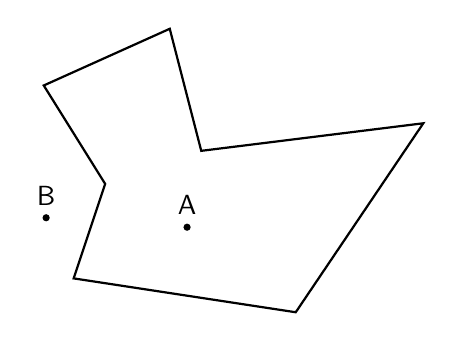
\begin{tikzpicture}[font=\sffamily]
\draw[thick] (3.30,-1.18)--(1.70,-1.90)--(2.48,-3.15)--(2.08,-4.35)--(4.90,-4.78)--(6.52,-2.38)--(3.70,-2.73)--cycle;
\fill (1.73,-3.58) circle (1.3pt) node[above=1pt] {B};
\fill (3.52,-3.70) circle (1.3pt) node[above=1pt] {A};
\end{tikzpicture}\\ Figure 3: A Polygon and two points\end{center}
\end{pastexam}

\section{實作練習}
\label{sec:dc-practice}

下面是 Aki-Judge 上和本章相關的題目。 兩題二分搜尋、「模冪函式」和「耗體力的淘汰
賽對戰表」只交函式（標頭檔或 \texttt{.c} 檔），不寫 \texttt{main}；其他題自己讀輸
入。

\begin{center}
\begin{tabular}{llc}
\toprule
小節 & 題目 & 難度 \\
\midrule
二分搜尋 & \akiref{binary-search-index-function}{二分搜尋索引函式} & 暖身 \\
 & \akiref{lower-and-upper-bound-in-a-sorted-array}{已排序陣列的下界與上界} & 基本 \\
快速冪 & \akiref{modular-exponentiation-function}{模冪函式} & 基本 \\
 & \akiref{fibonacci-number-modulo-1000000007}{費氏數列取模} & 進階 \\
最大子陣列 & \akiref{maximum-contiguous-subarray-sum}{最大連續子陣列和} & 基本 \\
 & \akiref{largest-contiguous-sum}{連續區段的最大和} & 基本 \\
最近點對 & \akiref{smallest-gap-between-points-on-a-line}{數線上最近兩點的距離} & 基本 \\
分治的結構 & \akiref{heavier-half-first}{重的一半排前面} & 基本 \\
 & \akiref{stamina-knockout-bracket}{耗體力的淘汰賽對戰表} & 進階 \\
\bottomrule
\end{tabular}
\end{center}

幾題的提示。 兩題二分搜尋的位置從 $0$ 開始，「二分搜尋索引函式」找不到回傳 $-1$，
「已排序陣列的下界與上界」找不到回傳 $n$；交之前用第~\ref{sec:dc-traps}~節列的小例子
自己測。 「模冪函式」的指數到 $10^{12}$，先把底數取餘數，指數是 $0$ 時回傳 $1$。
「費氏數列取模」用第~\ref{sec:dc-power}~節的矩陣快速冪，每次乘法和加法之後都取餘
數。 兩題最大子陣列都要求非空的段，用 \texttt{long long}；第一題用分治版，第二題的
$n$ 到 $10^6$，用線性版。 「數線上最近兩點的距離」是一維的最近點對，座標可以重複。
最後兩題都是「切成兩半、兩半各自處理完、再由兩半的結果決定這一段」，先寫出遞迴式再
動手；「耗體力的淘汰賽對戰表」要用 \texttt{malloc} 建出整棵遞迴樹，上半區是
$\lceil m/2 \rceil$ 人。 逆序數的兩題在第~14~章的題單，可以用 \proc{Sort-Count} 再
做一次。

\section{讀完你應該會}
\label{sec:dc-checklist}

\begin{itemize}
\item 寫出閉區間和半開區間的二分搜尋、\proc{Lower-Bound}、\proc{Upper-Bound}，用迴圈
不變量證明正確，並用它們算出現次數、最後一個不大於 $x$ 的位置等邊界問題；看得出
混用區間寫法、$\mathit{lo} \gets \mathit{mid}$ 配地板造成的無窮迴圈。
\item 寫出遞迴和迴圈兩種快速冪，算出乘法次數 $\lfloor \lg n \rfloor + \nu(n) - 1$，
在取餘數時不溢位，並能把同樣的方法用在矩陣上。
\item 用分治法和線性做法解最大子陣列，寫出跨中點的兩列累加，說明線性做法的
$E[i]$ 遞迴為什麼對。
\item 手算 Karatsuba 的三個乘積和 Strassen 的七個乘積，寫出它們的遞迴式，用主定理
說明為什麼少一次乘法就改變了指數。
\item 說明最近點對的帶狀區域為什麼寬 $2\delta$、每個點為什麼最多往後看 $7$ 個點，
並能手算每一層的 $x_m$、帶狀區域和比較的點對。
\item 用合併排序在 $\Theta(n \lg n)$ 內數逆序數，說明相等時為什麼要先拿左邊。
\item 用外積判斷左轉、右轉、共線；寫出線段相交的四個外積，說明 \proc{On-Segment} 為什
麼需要；用射線法判斷點在不在多邊形裡，處理射線通過頂點和水平邊的情形。
\item 手算 Graham 掃描法的排序和堆疊的每一步，說明它是 $\Theta(n \lg n)$ 而掃描只要
$O(n)$；說出分治凸包怎麼用兩條橋合併；用排序歸約證明凸包的 $\Omega(n \lg n)$ 下界；
知道最遠點對的兩點都在凸包上。
\end{itemize}

\textbf{延伸閱讀}（書末會整理完整的參考資料）

\begin{itemize}
\item Thomas H. Cormen 等，\textit{Introduction to Algorithms}，第 4 版，4.1、4.2 節：
矩陣乘法的分治版和 Strassen 演算法，Strassen 的七個乘積用另一組式子寫；章末問題
2-4 是逆序數。
\item Steven S. Skiena，\textit{The Algorithm Design Manual}，第 3 版，5.1、5.5、
5.6 節：二分搜尋的各種變化、快速乘法、最大子陣列與最近點對，用很短的篇幅講直覺。
\item Jon Kleinberg、Éva Tardos，\textit{Algorithm Design}，第 5 章：逆序數、最近點
對、整數乘法三節，最近點對的證明用了另一種切格子的方法，可以和本章對照。
\item Jon Bentley，\textit{Programming Pearls}，第 2 版，第 4 欄與第 8 欄：前者用二分
搜尋示範怎麼寫出正確的程式，後者從 $\Theta(n^3)$ 一路改進最大子陣列到線性時間。
\item Donald E. Knuth，\textit{The Art of Computer Programming, Vol.~2: Seminumerical
Algorithms}，第 3 版，4.3.3 節（快速乘法）與 4.6.3 節（冪的計算）：後者討論算 $x^n$
最少要幾次乘法，二進位法不一定最少（觀念題第~\ref{dc-q-pow}~題）。
\item Thomas H. Cormen 等，\textit{Introduction to Algorithms}，第 3 版，第 33 章：外積、
線段相交（含掃描線判斷 $n$ 條線段）、Graham 掃描法和禮物包裝法。 第 4 版刪掉了這一章。
\item Franco P. Preparata、Michael Ian Shamos，\textit{Computational Geometry: An
Introduction}，Springer，1985：凸包的各種做法與下界、點集的直徑（最遠點對）、線段相交
的掃描線演算法，舊卷的計算幾何題大多出自這本書的範圍。
\item Mark de Berg、Otfried Cheong、Marc van Kreveld、Mark Overmars，\textit{Computational
Geometry: Algorithms and Applications}，第 3 版，Springer，2008，第 1、2 章：凸包（包括
共線點和數值誤差怎麼處理）和線段相交的掃描線演算法。
\end{itemize}

\addcontentsline{toc}{section}{觀念題解答}
\section*{觀念題解答}

\begin{enumerate}
\item (a)、(d)、(e) 正確。

(a)：$k = \mathit{hi} - \mathit{lo} + 1$ 格時，$\mathit{mid}$ 左邊約 $2k/3$ 格、右邊
約 $k/3$ 格，最壞每輪剩下不超過約 $2k/3$，輪數不超過 $\log_{3/2} n + O(1)$；每輪
至多縮成三分之一，輪數也至少約 $\log_3 n$（$x$ 不在陣列裡時）。 兩者都是
$\Theta(\lg n)$，只差底數。

(b)：$T(n) = 6T(n/3) + \Theta(n)$，$\log_3 6 \approx 1.631 > \lg 3 \approx 1.585$，
比 Karatsuba 慢。 要比 Karatsuba 快，三段的切法最多只能用 $5$ 次乘法
（$\log_3 5 \approx 1.465$）。

(c)：$8T(n/2) + \Theta(n^2) = \Theta(n^3)$。 加法的次數只影響 $f(n)$ 的常數，決定指
數的是乘法的次數。

(d)：$T(n) = 2T(n/2) + \Theta(n^2)$，$n^2 = \Omega(n^{1 + \varepsilon})$，正則條件
$2(n/2)^2 = \frac{1}{2} n^2$，主定理情況 3 給出 $\Theta(n^2)$。

(e)：帶狀區域最多 $n$ 個點，重排 $O(n \lg n)$，$T(n) = 2T(n/2) + O(n \lg n) =
O(n \lg^2 n)$（定理~\ref{thm:rec-master2}，$k = 1$）。

\item 三次搜尋每一輪的值如下表。
\begin{center}
\begin{tabular}{cccccl}
\toprule
& $\mathit{lo}$ & $\mathit{hi}$ & $\mathit{mid}$ & $A[\mathit{mid}]$ & 動作 \\
\midrule
\proc{Lower-Bound}$(8)$ & 1 & 10 & 5 & 8 & $8 \ge 8$，$\mathit{hi} \gets 5$ \\
& 1 & 5 & 3 & 8 & $\mathit{hi} \gets 3$ \\
& 1 & 3 & 2 & 8 & $\mathit{hi} \gets 2$ \\
& 1 & 2 & 1 & 3 & $3 < 8$，$\mathit{lo} \gets 2$；回傳 $2$ \\
\midrule
\proc{Upper-Bound}$(8)$ & 1 & 10 & 5 & 8 & $8 \le 8$，$\mathit{lo} \gets 6$ \\
& 6 & 10 & 8 & 20 & $20 > 8$，$\mathit{hi} \gets 8$ \\
& 6 & 8 & 7 & 20 & $\mathit{hi} \gets 7$ \\
& 6 & 7 & 6 & 14 & $\mathit{hi} \gets 6$；回傳 $6$ \\
\midrule
\proc{Lower-Bound}$(21)$ & 1 & 10 & 5 & 8 & $8 < 21$，$\mathit{lo} \gets 6$ \\
& 6 & 10 & 8 & 20 & $20 < 21$，$\mathit{lo} \gets 9$ \\
& 9 & 10 & 9 & 27 & $27 \ge 21$，$\mathit{hi} \gets 9$；回傳 $9$ \\
\bottomrule
\end{tabular}
\end{center}
$8$ 出現 $6 - 2 = 4$ 次。 陣列裡沒有 $21$，所以「最後一個不大於 $21$」等於「最後一
個小於 $21$」，是 \proc{Lower-Bound}$(21) - 1 = 8$，$A[8] = 20$。 （用
\proc{Upper-Bound}$(21) - 1$ 也一樣是 $8$。）

\item
\begin{enumerate}
\item $A = \langle 4, 9 \rangle$，$x = 9$。 $\mathit{lo} = 1$、$\mathit{hi} = 2$，
$\mathit{mid} = 1$，$A[1] = 4 \le 9$，$\mathit{lo} \gets 1$，什麼都沒變，永遠重複。 只
要範圍剩兩格、左邊那格不大於 $x$，就會發生。
\item 把第 4 行改成 $\mathit{mid} \gets \lceil (\mathit{lo} + \mathit{hi}) / 2
\rceil$。 不變量：每次檢查第 3 行時，$1 \le \mathit{lo} \le \mathit{hi} \le n$，
$A[\mathit{lo}] \le x$，而且 $A[\mathit{hi}+1..n]$ 都大於 $x$。 初始：
$\mathit{lo} = 1$，題目保證 $A[1] \le x$；$A[n+1..n]$ 是空的。 維持：
$\mathit{lo} < \mathit{hi}$ 時 $\mathit{lo} < \mathit{mid} \le \mathit{hi}$。 若
$A[\mathit{mid}] \le x$，新的 $\mathit{lo} = \mathit{mid}$ 仍滿足 $A[\mathit{lo}] \le
x$；否則 $A[\mathit{mid}..n]$ 都大於 $x$，新的 $\mathit{hi} = \mathit{mid} - 1 \ge
\mathit{lo}$，第二段仍成立。 結束：$\mathit{lo} = \mathit{hi}$，$A[\mathit{lo}] \le
x$ 而 $A[\mathit{lo}+1..n]$ 都大於 $x$，$\mathit{lo}$ 正是最後一個不大於 $x$ 的位
置。 會停：每輪 $\mathit{lo}$ 嚴格變大（$\mathit{mid} > \mathit{lo}$）或
$\mathit{hi}$ 嚴格變小，$\mathit{hi} - \mathit{lo}$ 是非負整數，有限輪後變成 $0$。
\item \proc{Upper-Bound}$(A, n, x) - 1$。 這個寫法不需要「$A[1] \le x$」的保證，
全部都大於 $x$ 時回傳 $0$。
\end{enumerate}

\item
\begin{enumerate}
\item $100 = 1100100_2$。
\begin{center}
\begin{tabular}{cccl}
\toprule
$e$ & $r$ & $b$ & 這一輪 \\
\midrule
100 & 1 & $3$ & 偶數；$b \gets 3^2$ \\
50 & 1 & $3^2$ & 偶數；$b \gets 3^4$ \\
25 & 1 & $3^4$ & 奇數：$r \gets 3^4$；$b \gets 3^8$ \\
12 & $3^4$ & $3^8$ & 偶數；$b \gets 3^{16}$ \\
6 & $3^4$ & $3^{16}$ & 偶數；$b \gets 3^{32}$ \\
3 & $3^4$ & $3^{32}$ & 奇數：$r \gets 3^{36}$；$b \gets 3^{64}$ \\
1 & $3^{36}$ & $3^{64}$ & 奇數：$r \gets 3^{100}$；$e$ 變成 $0$，不再平方 \\
\bottomrule
\end{tabular}
\end{center}
第 5 行執行 $\nu(100) = 3$ 次，第 8 行執行 $\lfloor \lg 100 \rfloor = 6$ 次，共 $9$ 次。
\item $\lfloor \lg 15 \rfloor + \nu(15) - 1 = 3 + 3 = 6$ 次（$x^2$、$x^3$、$x^6$、
$x^7$、$x^{14}$、$x^{15}$）。 $5$ 次的方法：$x^2 = x \cdot x$，$x^3 = x^2 \cdot x$，
$x^6 = x^3 \cdot x^3$，$x^{12} = x^6 \cdot x^6$，$x^{15} = x^{12} \cdot x^3$。 二進位
法不一定用最少的乘法。 最少要幾次沒有簡單的公式，但任何方法至少要 $\lceil \lg n
\rceil$ 次（每次乘法最多讓指數加倍），二進位法不超過 $2\lfloor \lg n \rfloor$ 次，
最多差一倍左右。
\end{enumerate}

\item
\begin{enumerate}
\item $q = 4$。 往左累加（從第 4 個往左）：$4, 3, 8, 5$，最大 $8$（第 2 到 4 個）；往
右累加（從第 5 個往右）：$-7, -1, -3$，最大 $-1$（第 5 到 6 個）。
\proc{Max-Crossing} 回傳第 2 到 6 個，和 $7$。 左半 $\langle -3, 5, -1, 4 \rangle$ 的
最佳段是第 2 到 4 個，和 $8$；右半 $\langle -7, 6, -2 \rangle$ 是第 6 個，和 $6$。
答案是第 2 到 4 個，和 $8$，來自左半。 往右累加的最大值是負的，但跨中點的段一定要
包含第 5 個，所以只能取 $-1$。
\item 每一輪結束時的值如下表，答案同樣是第 2 到 4 個，和 $8$。
\begin{center}
\begin{tabular}{cccl}
\toprule
$i$ & $A[i]$ & $\mathit{cur}$ & $\mathit{best}$ \\
\midrule
1 & $-3$ & $-3$ & 1--1：$-3$ \\
2 & 5 & 重新開始：5 & 2--2：5 \\
3 & $-1$ & 4 & 2--2：5 \\
4 & 4 & 8 & 2--4：8 \\
5 & $-7$ & 1 & 2--4：8 \\
6 & 6 & 7 & 2--4：8 \\
7 & $-2$ & 5 & 2--4：8 \\
\bottomrule
\end{tabular}
\end{center}
\end{enumerate}

\item
\begin{enumerate}
\item $T = T_L + T_R$。 $P = \max(P_L,\ T_L + P_R)$：開頭在最左邊的段，要嘛整段在左
半，要嘛包含整個左半再接右半的一個前綴。 $S = \max(S_R,\ T_R + S_L)$，理由對稱。
$M = \max(M_L,\ M_R,\ S_L + P_R)$：最後一項就是引理~\ref{lem:dc-crossing}，左半的最佳
後綴正是「結尾在 $q$ 的最佳段」。 基礎情況一個數 $a$：四個值都是 $a$。
\item 合併只要常數時間，$T(n) = 2T(n/2) + \Theta(1)$，主定理情況 1，$\Theta(n)$。
第~\ref{sec:dc-maxsub}~節的版本每一層從中點重新往兩邊加，花 $\Theta(n)$；這裡讓子問
題把以後會用到的前綴、後綴資訊一起交回來，合併時就不必再看陣列。
\end{enumerate}

\item 七個乘積：
\[
\begin{aligned}
M_1 &= (2 + 4)(2 + (-1)) = 6, & M_2 &= (1 + 4) \times 2 = 10, \\
M_3 &= 2 \times (0 - (-1)) = 2, & M_4 &= 4 \times (5 - 2) = 12, \\
M_5 &= (2 + (-3)) \times (-1) = 1, & M_6 &= (1 - 2)(2 + 0) = -2, \\
M_7 &= (-3 - 4)(5 + (-1)) = -28.
\end{aligned}
\]
$c_{11} = 6 + 12 - 1 + (-28) = -11$，$c_{12} = 2 + 1 = 3$，$c_{21} = 10 + 12 = 22$，
$c_{22} = 6 - 10 + 2 + (-2) = -4$。 驗算：$c_{11} = 2 \cdot 2 + (-3) \cdot 5 = -11$，
$c_{12} = 2 \cdot 0 + (-3)(-1) = 3$，$c_{21} = 1 \cdot 2 + 4 \cdot 5 = 22$，
$c_{22} = 1 \cdot 0 + 4 \cdot (-1) = -4$。

\item 最上層 $q = 4$，$x_m = 9$（D 的 $x$）。 D 落在分界線上，屬於左半（左半是依
$x$ 排序後的前 $4$ 個點）。 左半 A、B、C、D 的最近距離平方是 BC $= 16$，右半 E、F、
G、H 是 FH $= 9 + 4 = 13$，$\delta^2 = 13$。 帶狀區域 $(x - 9)^2 < 13$：C（$4$）、
D（$0$）、E（$1$）、F（$4$），B（$36$）和 G（$16$）不在。 依 $y$ 排：C(7, 7)、
E(10, 7)、F(11, 11)、D(9, 12)，C 和 E 的 $y$ 相同，依 $x$ 排。 比較：
\begin{itemize}
\item C 往後：CE，$y$ 差 $0$，距離平方 $9 < 13$，$\delta^2 \gets 9$；下一個 F 的
$y$ 差 $4$，$16 \ge 9$，停。
\item E 往後：F 的 $y$ 差 $4$，$16 \ge 9$，停，沒有算距離。
\item F 往後：FD，$y$ 差 $1$，距離平方 $4 + 1 = 5 < 9$，$\delta^2 \gets 5$。
\end{itemize}
答案是 F、D，距離 $\sqrt{5}$。 這一層 $\delta$ 在迴圈裡變小了兩次，第一次（CE）找
到的也是跨兩半的點對，但還不是最近的。

\item
\begin{enumerate}
\item 依遞迴的完成順序：$A[1..2]$：$1$（$(5, 1)$）；$A[3..4]$：$1$（$(7, 3)$）；
$A[1..4]$：$\langle 1, 5 \rangle$ 和 $\langle 3, 7 \rangle$，$1$（$(5, 3)$）；
$A[5..6]$：$0$；$A[7..8]$：$0$；$A[5..8]$：$\langle 3, 8 \rangle$ 和
$\langle 2, 6 \rangle$，$3$（$(3, 2)$、$(8, 2)$、$(8, 6)$）；最上層 $6$。 總數
$1 + 1 + 1 + 0 + 0 + 3 + 6 = 12$。
\item 合併 $\langle 1, 3, 5, 7 \rangle$ 和 $\langle 2, 3, 6, 8 \rangle$：
$1$ 對 $2$，拿左 $1$；$3$ 對 $2$，拿右 $2$，左半還沒拿的 $3, 5, 7$，$+3$；$3$ 對 $3$，
相等，拿左 $3$；$5$ 對 $3$，拿右 $3$，還沒拿的 $5, 7$，$+2$；$5$ 對 $6$，拿左 $5$；
$7$ 對 $6$，拿右 $6$，$+1$；$7$ 對 $8$，拿左 $7$；左半用完，拿右 $8$，$+0$。 共
$6$。
\item 改成 $<$ 之後，$3$ 對 $3$ 時先拿右邊的 $3$，左半還沒拿的是 $3, 5, 7$，加 $3$
而不是 $2$；其他層的合併沒有相等的情形。 總數變成 $13$，多算了左半的 $3$ 和右半的
$3$ 這一對，它們相等，不是逆序。
\end{enumerate}

\item
\begin{enumerate}
\item $Q - P = (5, 2)$。 $R - P = (2, 5)$：$5 \cdot 5 - 2 \cdot 2 = 21 > 0$，左轉。
$S - P = (10, 4)$：$5 \cdot 4 - 2 \cdot 10 = 0$，共線（$S - P$ 正好是 $Q - P$ 的兩倍，
$Q$ 在 $P$、$S$ 之間）。
\item 三組的結果：
\begin{center}
\begin{tabular}{lccccl}
\toprule
線段 & $d_1$ & $d_2$ & $d_3$ & $d_4$ & 結果 \\
\midrule
$\overline{PS}$、$\overline{QR}$ & $21$ & $-21$ & $0$ & $42$ & 第 11 行，\TRUE \\
$\overline{PR}$、$\overline{QS}$ & $0$ & $21$ & $-21$ & $-42$ & 第 14 行，\FALSE \\
$\overline{RT}$、$\overline{PS}$ & $42$ & $-48$ & $-39$ & $51$ & 第 5 行，\TRUE \\
\bottomrule
\end{tabular}
\end{center}
第一組：$d_1 d_2 < 0$ 但 $d_3 = 0$，第 4 行不成立；$d_1$、$d_2$ 不是 $0$；$d_3 = 0$ 且
$Q = (7, 5)$ 在以 $P$、$S$ 為對角的長方形裡（$2 \le 7 \le 12$、$3 \le 5 \le 7$），第 11
行回傳 \TRUE：$\overline{QR}$ 的端點 $Q$ 碰到 $\overline{PS}$。 第二組：$d_1 = 0$，
$P$ 在直線 $QS$ 上，但 $P.x = 2$ 不在 $[7, 12]$ 裡，不在線段上；其他三個 $d$ 都不是
$0$，第 4 行也不成立（$d_1 d_2 = 0$），所以第 14 行回傳 \FALSE。 第三組四個外積都不
是 $0$，$d_1 d_2 < 0$、$d_3 d_4 < 0$，互相跨過。
\item 第二組。 $d_1 = 0$ 只表示 $P$ 在直線 $QS$ 上；$P$ 在 $Q$ 的另一側、線段
$\overline{QS}$ 外面，兩條線段其實沒有碰到。
\end{enumerate}

\item
\begin{enumerate}
\item 高度等於 $4$ 的頂點 $v_3, v_4, v_6$ 都算在下方，所以只有 $v_4 v_5$、$v_5 v_6$ 兩條
邊跨過（它們的上端是 $v_5$），水平邊 $v_3 v_4$ 和 $v_2 v_3$、$v_6 v_1$ 都不算。
\begin{center}
\begin{tabular}{lcccc}
\toprule
& 邊 & $\proc{Orient}(a, b, q)$ & $b.y - a.y$ & 乘積 \\
\midrule
$q_1(2, 4)$ & $v_4 v_5$ & $12$ & $3$ & $36$ \\
& $v_5 v_6$ & $-3$ & $-3$ & $9$ \\
\midrule
$q_2(4, 4)$ & $v_4 v_5$ & $6$ & $3$ & $18$ \\
& $v_5 v_6$ & $3$ & $-3$ & $-9$ \\
\bottomrule
\end{tabular}
\end{center}
$q_1$ 兩個乘積都是正的，$c = 2$，在外面：射線在 $v_6$ 穿進多邊形，在 $v_4$ 穿出去，
之後沿著水平邊 $v_3 v_4$ 走，沒有再穿過邊界。 $q_2$ 只有 $v_4 v_5$ 算，$c = 1$，在裡
面（$v_5 v_6$ 和射線的交點是 $v_6$，在 $q_2$ 左邊）。
\item 改成 $\ge$ 之後，$v_3, v_4, v_6$ 都算在上方，跨過的邊變成 $v_2 v_3$ 和 $v_6 v_1$。
$q_1$：$v_2 v_3$ 的乘積 $21 \cdot 3 = 63 > 0$，$v_6 v_1$ 的乘積 $(-3)(-3) = 9 > 0$，
$c = 2$，在外面。 $q_2$：$v_2 v_3$ 的乘積 $15 \cdot 3 = 45 > 0$，$v_6 v_1$ 的乘積
$3 \cdot (-3) = -9$，不算，$c = 1$，在裡面。 數到的邊不一樣，但奇偶相同，答案仍然正
確。 原因是規則只要求「每個剛好在射線高度的頂點，一律歸到同一邊」，歸到上方或下方都
可以。
\end{enumerate}

\item
\begin{enumerate}
\item $A$、$B$ 的 $y$ 都是 $0$，取 $x$ 小的，$p_0 = B$。 排序：$A$（極角 $0^\circ$）、$C$、
$D$、$H$、$E$、$F$、$G$。 $H - B = (1, 4)$ 和 $E - B = (2, 8)$ 方向相同，$H$ 比較近，排在
前面。
\begin{center}
\begin{tabular}{clll}
\toprule
處理 & 彈出（外積） & 堆疊（底 $\to$ 頂） & 說明 \\
\midrule
（開始） & & $B, A$ & \\
$C$ & & $B, A, C$ & $\proc{Orient}(B, A, C) = 16$ \\
$D$ & & $B, A, C, D$ & $\proc{Orient}(A, C, D) = 10$ \\
$H$ & $D$（$-5$） & $B, A, C, H$ & $\proc{Orient}(A, C, H) = 20$ \\
$E$ & $H$（$-20$） & $B, A, C, E$ & $\proc{Orient}(A, C, E) = 24$ \\
$F$ & & $B, A, C, E, F$ & $\proc{Orient}(C, E, F) = 24$ \\
$G$ & & $B, A, C, E, F, G$ & $\proc{Orient}(E, F, G) = 14$ \\
\bottomrule
\end{tabular}
\end{center}
凸包是 $B, A, C, E, F, G$（逆時針）。 $H$ 在線段 $\overline{BE}$ 上，處理 $E$ 時被彈掉；
$D$ 在凸包內部。
\item 例子：$p_0 = (0, 0)$、$(10, 0)$，再把五個點放在一段向外凸的弧
上：$(9, 4)$、$(8, 6)$、$(6, 8)$、$(4, 9)$、$(1, 10)$，最後一點 $(0, 100)$ 放在很高的地
方。 前七個點依極角處理時每一步都是左轉，堆疊長到七個點；$(0, 100)$ 進來時，那五個點
都在三角形 $(0, 0)$、$(10, 0)$、$(0, 100)$ 裡面，依序被彈出（外積分別是 $-269$、
$-178$、$-172$、$-78$、$-60$），凸包只剩三個點。 即使如此，每個點只推入一次、最多彈
出一次，整個掃描的彈出總數不超過 $n$，第 6 行的檢查總數不超過 $2n$。 某一步很貴，是
因為前面幾步很便宜、累積了很多點在堆疊裡，這正是聚合法的論證。
\end{enumerate}

\item
\begin{enumerate}
\item 令 $u = a - q$、$v = b - q$，則 $p - q = t u + (1 - t) v$。 用內積展開：
\[
|p - q|^2 = t^2 |u|^2 + (1 - t)^2 |v|^2 + 2t(1 - t)\, u \cdot v .
\]
右邊的式子是
\[
t|u|^2 + (1 - t)|v|^2 - t(1 - t)\bigl(|u|^2 + |v|^2 - 2 u \cdot v\bigr),
\]
其中 $|a - b|^2 = |u - v|^2 = |u|^2 + |v|^2 - 2u \cdot v$。 $|u|^2$ 的係數是
$t - t(1 - t) = t^2$，$|v|^2$ 的係數是 $(1 - t) - t(1 - t) = (1 - t)^2$，$u \cdot v$
的係數是 $2t(1 - t)$，兩邊相同。
\item $a \ne b$、$0 < t < 1$ 時最後一項 $t(1 - t)|a - b|^2 > 0$，所以
$|p - q|^2 < t|a - q|^2 + (1 - t)|b - q|^2 \le \max(|a - q|, |b - q|)^2$（兩個數的加權平
均不超過較大的那個），開根號即得。
\item 設 $(p, q)$ 是一組最遠點對，假設 $p$ 不是凸包的頂點。 $p$ 在凸包（含內部）裡，
分兩種情形找一條線段 $\overline{cd}$，讓 $p$ 嚴格在 $c$、$d$ 之間，而 $c$、$d$ 都在凸
包的邊界上：$p$ 在某條邊上（不是端點）時，取那條邊；$p$ 在內部時，過 $p$ 任畫一條直
線，它和凸包的交集是一條線段，兩端在邊界上。 由 (b)，$c$、$d$ 中有一個（設為 $c$）
滿足 $|c - q| > |p - q|$。 如果 $c$ 是頂點，令 $w = c$；否則 $c$ 在某條邊
$\overline{uv}$ 的內部，再用一次 (b)，$u$、$v$ 中有一個（設為 $w$）滿足
$|w - q| > |c - q|$。 不論哪一種，$w$ 都是凸包的頂點，也是點集裡的點，而
$|w - q| > |p - q|$，和 $(p, q)$ 最遠矛盾。 所以 $p$ 是頂點；$q$ 同理。
\item $O(n \lg n + h^2)$。 $h^2 = O(n \lg n)$，也就是 $h = O(\sqrt{n \lg n})$ 時，總時間
仍是 $O(n \lg n)$。 $h$ 可以大到 $n$（點都在一個圓上），這時是 $\Theta(n^2)$，所以需要
旋轉卡尺。
\end{enumerate}

\end{enumerate}

\addcontentsline{toc}{section}{歷屆試題詳解}
\section*{歷屆試題詳解}

\pastsol{px:dc-1}{臺大資工所 111 學年度 第 10 題}
答案是 (C)。

第 1 行保證進入迴圈時 $A[1] > 0$，所以 $p \ge 1$。 正數恰好是前 $p$ 個，因此
$A[m] > 0$ 等價於 $m \le p$，$A[m] < 0$ 等價於 $m \ge p + 1$（題目說每個元素不是正就
是負，沒有 $0$）。 照第~\ref{sec:ana-invariant}~節的三步驗證 (C)：

\begin{itemize}
\item \textbf{初始}：$left = 1 \le p$，$p \le n = right$。
\item \textbf{維持}：迴圈裡 $left < right$，$m = \lceil (left + right)/2 \rceil$ 滿足
$left < m \le right$。 若 $A[m] > 0$，則 $m \le p$，新的 $left = m \le p$，$right$ 不變；
若 $A[m] < 0$，則 $m \ge p + 1$，新的 $right = m - 1 \ge p$，$left$ 不變。 兩種情形
$left \le p \le right$ 都仍成立。
\item \textbf{結束}：每一輪 $left$ 嚴格變大（$m > left$）或 $right$ 嚴格變小，迴圈一定會
停，停在 $left = right$，代入不變量得 $p = left$，第 9 行回傳正確。
\end{itemize}

其他選項：

\begin{itemize}
\item (A) $left + 1 \le p$：$p = 1$ 時（例如 $A = \langle 5, -2 \rangle$），一開始
$left = 1$，$left + 1 = 2 > p$，第一次檢查就不成立。 而且迴圈結束時 $left = p$，這個不
等式一定不成立。
\item (B) 比 (A) 多要求 $p \le right - 1$，同樣在 $p = 1$ 時一開始就不成立；結束時
$left = right$，$left + 1 \le right - 1$ 不可能成立。
\item (D) $p \le right - 1$：全部都是正數時（例如 $A = \langle 3, 1 \rangle$，$p = n = 2$），
一開始 $right = 2$，$p \le 1$ 不成立。 結束時 $left = right$，$left \le p \le left - 1$ 也
不可能成立。
\item (E)：(C) 成立，所以不選。
\end{itemize}

用程式把 $n \le 8$ 的所有情形（每個 $n$、每個 $p$）跑過，每一輪檢查四個不等式，只
有 (C) 每次都成立。 這個程序就是觀念題第~\ref{dc-q-fix}~題改好的「最後一個滿足條件的位
置」：往右縮寫成 $left = m$，所以中點一定要取天花板（第~\ref{sec:dc-traps}~節）。 如果第
4 行改成地板，$left = 1$、$right = 2$、$A[1] > 0$ 時 $m = 1$，$left$ 不動，迴圈不會停。

\pastsol{px:dc-2}{中正資工所 111 學年度 第 1 題}
答案是 (c)。

照考卷的慣例，二分搜尋每一輪把 $x$ 和中間那一格比一次（相等、較小、較大三種結果算一
次比較）。 第~\ref{sec:dc-bsearch}~節證明了：還要找的格數 $k$ 每一輪之後最多剩
$\lfloor k/2 \rfloor$，所以迴圈最多跑 $\lfloor \lg n \rfloor + 1$ 輪。
$2^{10} = 1024 \le 2000 < 2048 = 2^{11}$，$\lfloor \lg 2000 \rfloor = 10$，最多 $11$ 次。

這個上界達得到：$x$ 比全部都大時每一輪都往右，格數依序是
$2000 \to 1000 \to 500 \to 250 \to 125 \to 62 \to 31 \to 15 \to 7 \to 3 \to 1 \to 0$，
每個箭頭是一次比較，共 $11$ 次（用程式對 $2000$ 格的陣列試過所有位置和所有落在兩格之間
的值，最多正好 $11$ 次）。

\begin{itemize}
\item (a) $1999$：這是循序搜尋那一級的次數，二分搜尋不需要。
\item (b) $9$：上面的例子做完 $9$ 次比較後還剩 $3$ 格沒找，無法確定答案。
\item (d) $13$：比最壞情況還多。
\end{itemize}

如果把「是否相等」和「是否較小」算成兩次比較，最壞是 $22$ 次，不在選項裡，所以題目
用的是一輪算一次的算法。

\pastsol{px:dc-3}{成大資訊聯招 113 學年度 第 11 題}
$T(n) = \Theta(n^{\lg 7})$，$\lg 7 \approx 2.807$。

\textbf{寫出遞迴式}。 $n = 1$ 時做一次乘法，$\Theta(1)$。 $n \ge 2$ 時：
\begin{itemize}
\item 遞迴呼叫：$C_{11}$、$C_{12}$、$C_{21}$ 各兩次，$C_{22}$ 一次，共 $7$ 次，每次的
矩陣是 $\frac{n}{2} \times \frac{n}{2}$，合計 $7T(n/2)$。
\item 矩陣加法：$C_{11}$、$C_{12}$、$C_{21}$ 各一次，每次是 $\frac{n}{2} \times \frac{n}{2}$
的 $(n/2)^2$ 次加法，合計 $3n^2/4 = \Theta(n^2)$。
\item 切塊和組合 $C$：用下標計算切塊是 $\Theta(1)$，把子矩陣複製出來是 $\Theta(n^2)$；
組合 $C$ 最多 $\Theta(n^2)$。 不論哪一種實作都是 $O(n^2)$，和加法合起來仍是
$\Theta(n^2)$。
\end{itemize}
所以
\[
T(n) = 7T(n/2) + \Theta(n^2).
\]

\textbf{解遞迴式}。 $a = 7$、$b = 2$，$n^{\log_b a} = n^{\lg 7}$。 $\lg 7 \approx 2.807$，取
$\varepsilon = 0.8$，$n^2 = O(n^{\lg 7 - 0.8})$（$\lg 7 - 0.8 \approx 2.007 > 2$），主定理
情況 1（定理~\ref{thm:rec-master}）給出 $T(n) = \Theta(n^{\lg 7})$。

用遞迴樹檢查：第 $i$ 層有 $7^i$ 個子問題，每個的加法成本是 $c(n/2^i)^2$，整層是
$cn^2 (7/4)^i$，是公比 $7/4 > 1$ 的等比數列，總和由最後一層決定；最後一層有
$7^{\lg n} = n^{\lg 7}$ 個葉節點，每個 $\Theta(1)$。 兩種方法一致。

\textbf{說明}。 這個程序其實算錯了：正確的 $C_{22} = A_{21}B_{12} + A_{22}B_{22}$，它少了
$A_{22}B_{22}$。 但題目只問時間。 它的遞迴式和 Strassen 演算法（第~\ref{sec:dc-strassen}~節）
一樣，都是 $7$ 次半大的乘法加上 $\Theta(n^2)$ 的加減，所以時間也一樣；差別是 Strassen
用 $7$ 次乘法算出\textbf{正確}的四塊。 常見的錯誤是看到 $C_{11}$ 到 $C_{21}$ 各兩次就寫
$8T(n/2)$，要數清楚題目特別提醒的 $C_{22}$ 只呼叫一次。

\pastsol{px:dc-4}{政大資科所 107 學年度 第 7 題}
\textbf{解讀}。 題目允許長度 $0$ 的子序列，和是 $0$。 所以全部都是負數時，答案是空的子
序列（和 $0$），這和第~\ref{sec:dc-maxsub}~節「至少一個數」的約定不同。 輸出用位置
$i..j$ 表示 $a_i, \ldots, a_j$，空的子序列寫成 $j = i - 1$。 多段一樣大時，回傳最先達到
最大和的那一段。

\textbf{想法}。 改寫第~\ref{sec:dc-kadane}~節的線性做法。 令
\[
F[j] = \text{結尾在 } j \text{ 的子序列（可以是空的）的最大和},
\]
$F[0] = 0$。 結尾在 $j$ 的非空子序列，是「結尾在 $j - 1$ 的子序列（可以是空的）」再接上
$a_j$，最大是 $F[j-1] + a_j$；再和空的比，$F[j] = \max(0,\ F[j-1] + a_j)$。 答案是所有
「結尾在 $j$ 的非空最佳和」$F[j-1] + a_j$ 和空序列的 $0$ 之中最大的。

\begin{pseudo}[label=alg:dc-px-maxsub]{最大和的連續子序列（允許空的）}
\Function{Max-Contiguous}{$a, n$}
    \State $\mathit{best} \gets 0$；$\mathit{bi} \gets 1$；$\mathit{bj} \gets 0$ \Comment{先記空的子序列}
    \State $\mathit{cur} \gets 0$；$\mathit{start} \gets 1$
    \For{$j \gets 1$ \To $n$}
        \State $\mathit{cur} \gets \mathit{cur} + a_j$
        \If{$\mathit{cur} > \mathit{best}$}
            \State $\mathit{best} \gets \mathit{cur}$；$\mathit{bi} \gets \mathit{start}$；$\mathit{bj} \gets j$
        \EndIf
        \If{$\mathit{cur} < 0$}
            \State $\mathit{cur} \gets 0$；$\mathit{start} \gets j + 1$ \Comment{接上前面只會更差}
        \EndIf
    \EndFor
    \State \Return $(\mathit{bi}, \mathit{bj}, \mathit{best})$
\EndFunction
\end{pseudo}

\textbf{正確性}。 不變量：第 4 行每一輪開始時，(i) $\mathit{cur} = F[j-1] =
a_{\mathit{start}} + \cdots + a_{j-1}$（$\mathit{start} = j$ 時是空的、和為 $0$）；
(ii) $(\mathit{bi}, \mathit{bj}, \mathit{best})$ 是 $a_1, \ldots, a_{j-1}$ 裡（可以是空
的）和最大的連續子序列。
\begin{itemize}
\item \textbf{初始}：$j = 1$，$\mathit{cur} = 0 = F[0]$，只有空的子序列，(i)(ii) 都成立。
\item \textbf{維持}：第 5 行之後 $\mathit{cur} = F[j-1] + a_j = a_{\mathit{start}} +
\cdots + a_j$，是結尾在 $j$ 的非空子序列的最大和。 $a_1..a_j$ 裡的子序列，不是在
$a_1..a_{j-1}$ 裡，就是結尾在 $j$ 的非空子序列，所以第 6--7 行之後 (ii) 對 $j$ 成立。
第 8--9 行把 $\mathit{cur}$ 變成 $\max(0, \mathit{cur}) = F[j]$：小於 $0$ 時換成空的子
序列，從 $j + 1$ 重新開始。 (i) 對下一輪成立。
\item \textbf{結束}：$j = n + 1$，由 (ii)，回傳的是整個 $S$ 裡和最大的連續子序列。
\end{itemize}

\textbf{時間}。 迴圈 $n$ 輪，每輪常數個動作，$\Theta(n)$；額外空間 $\Theta(1)$。 題目只要
求多項式時間，兩兩枚舉所有 $i \le j$ 邊走邊加的 $\Theta(n^2)$ 或第~\ref{sec:dc-maxsub}~節的
分治 $\Theta(n \lg n)$ 也都符合，但線性做法最好，而且不可能更快：每個數都可能是答案的一
部分，至少要讀過一次。

\textbf{追蹤題目的例子}。 $S = 5, 15, -30, 10, -5, 40, 10$。 表中「第 5 行後」是加上
$a_j$ 之後的 $\mathit{cur}$，「本輪結束」是第 8--9 行之後的值。
\begin{center}
\begin{tabular}{ccccl}
\toprule
$j$ & $a_j$ & 第 5 行後 & 本輪結束 & $(\mathit{bi}, \mathit{bj}, \mathit{best})$ \\
\midrule
1 & $5$ & $5$ & $5$ & $(1, 1, 5)$ \\
2 & $15$ & $20$ & $20$ & $(1, 2, 20)$ \\
3 & $-30$ & $-10$ & $0$，$\mathit{start} = 4$ & $(1, 2, 20)$ \\
4 & $10$ & $10$ & $10$ & $(1, 2, 20)$ \\
5 & $-5$ & $5$ & $5$ & $(1, 2, 20)$ \\
6 & $40$ & $45$ & $45$ & $(4, 6, 45)$ \\
7 & $10$ & $55$ & $55$ & $(4, 7, 55)$ \\
\bottomrule
\end{tabular}
\end{center}
回傳 $(4, 7, 55)$，也就是 $10, -5, 40, 10$，和 $55$，和題目給的答案相同。 也用程式把這個程序和兩兩枚舉在兩萬組隨機的小輸入上比對過，最大和都相同。 全部是負數時，例如
$-3, -1$，$\mathit{best}$ 一直是 $0$，回傳 $(1, 0, 0)$，即空的子序列。

\pastsol{px:dc-5}{臺大資工所 103 學年度 第 5 題（節錄 (a)(c) 小題）}
\textbf{(a)} 用外積判斷轉向，演算法就是第~\ref{sec:dc-segint}~節的
\proc{Segments-Intersect}（虛擬碼~\ref{alg:dc-segint}）：
\begin{enumerate}[label=\arabic*.]
\item 令 $\proc{Orient}(p, q, r) = (q.x - p.x)(r.y - p.y) - (q.y - p.y)(r.x - p.x)$，正、
負、零分別表示 $p \to q \to r$ 左轉、右轉、共線（第~\ref{sec:dc-orient}~節）。
\item 算 $d_1 = \proc{Orient}(p_3, p_4, p_1)$、$d_2 = \proc{Orient}(p_3, p_4, p_2)$、
$d_3 = \proc{Orient}(p_1, p_2, p_3)$、$d_4 = \proc{Orient}(p_1, p_2, p_4)$。
\item 如果 $d_1$、$d_2$ 異號而且 $d_3$、$d_4$ 異號，兩條線段互相跨過對方所在的直線，
回傳 TRUE。
\item 否則，如果某個 $d_k = 0$，而對應的端點落在另一條線段上（座標在另一條線段兩端點
圍成的長方形裡，即 \proc{On-Segment}），回傳 TRUE。 這涵蓋端點碰到另一條線段、以及四
點共線而且有重疊的情形。
\item 其他情形回傳 FALSE。
\end{enumerate}
正確性就是引理~\ref{lem:dc-segint}：第 3 步成立時兩條直線交於一點，而這一點同時在兩
條線段上；反過來，兩條線段有共同點而且沒有端點落在另一條線段上時，四個外積都不是 $0$，
而且兩兩異號。 第 4 步不能省：四點共線但分開時（圖~\ref{fig:dc-segcases} (d)），四個外積
都是 $0$，只有座標範圍的檢查能分辨。 只做 $4$ 次外積和常數次比較，$O(1)$；全部用整數
的乘法和減法，沒有除法，不會遇到斜率不存在或浮點誤差。

\textbf{(c)} 用射線法（第~\ref{sec:dc-pip}~節，虛擬碼~\ref{alg:dc-pip}）。

\textbf{想法}。 從點 $q$ 往右畫一條水平射線，數它和多邊形的邊相交幾次；奇數次在裡面，
偶數次在外面。 射線往右走到夠遠的地方一定在多邊形外面，每穿過一次邊界裡外就交換一次，
而多邊形沒有自我相交，邊界把平面分成裡外兩塊，所以奇偶決定答案。

\textbf{細節}。 逐一檢查每條邊 $(v_i, v_{i+1})$（最後一條是 $(v_n, v_1)$）：
\begin{itemize}
\item 只有兩端點一個嚴格在 $q.y$ 上方、另一個不在上方時才算這條邊跨過水平線
$y = q.y$。 高度剛好等於 $q.y$ 的頂點一律當成在下方，所以射線通過頂點時，穿過去的頂點
只算一次，只碰一下的頂點算 $0$ 次或 $2$ 次，水平邊不算，奇偶都正確。
\item 跨過的邊再判斷交點是否在 $q$ 的右邊：交點 $X$ 和 $q$ 同高，
$\proc{Orient}(v_i, v_{i+1}, q) = (v_{i+1}.y - v_i.y)(X.x - q.x)$，所以只要看
$\proc{Orient}(v_i, v_{i+1}, q)$ 和 $v_{i+1}.y - v_i.y$ 是否同號，不必做除法。 $q$ 不在
邊界上，所以這個乘積不會是 $0$。
\end{itemize}
題目說頂點依逆時針排列，射線法用不到這個條件，順時針也一樣。

\textbf{圖 3 的例子}。 依圖上的位置，從 $A$ 往右的射線只穿過右下方那條往右上的邊
（交點約在 $x = 5.6$），$1$ 次，奇數，$A$ 在裡面。 從 $B$ 往右的射線先穿過左邊往左下的
那條邊（交點約在 $x = 2.3$，在 $B$ 的右邊），再穿過同一條右下方的邊，$2$ 次，偶數，$B$
在外面。 這個多邊形不是凸的（左邊和上方各有一個凹進去的頂點），所以不能用下面凸多邊形
的二分搜尋。

\textbf{時間}。 每條邊做常數次運算，$n$ 個頂點的多邊形是 $\Theta(n)$，額外空間
$\Theta(1)$。 對一般的簡單多邊形，沒有事先處理時這已經是最好的：任何一條沒看過的邊都可
能改變答案，至少要讀過所有的邊。 如果多邊形是凸的，可以從 $v_1$ 把多邊形切成扇形，用二
分搜尋找 $q$ 落在哪個扇形，再做一次外積，$O(\lg n)$；同一個多邊形要回答很多次查詢時，
也可以先花時間建資料結構，讓每次查詢變快，這已經超出題目的範圍。
